% Options for packages loaded elsewhere
\PassOptionsToPackage{unicode}{hyperref}
\PassOptionsToPackage{hyphens}{url}
%
\documentclass[
]{book}
\usepackage{lmodern}
\usepackage{amssymb,amsmath}
\usepackage{ifxetex,ifluatex}
\ifnum 0\ifxetex 1\fi\ifluatex 1\fi=0 % if pdftex
  \usepackage[T1]{fontenc}
  \usepackage[utf8]{inputenc}
  \usepackage{textcomp} % provide euro and other symbols
\else % if luatex or xetex
  \usepackage{unicode-math}
  \defaultfontfeatures{Scale=MatchLowercase}
  \defaultfontfeatures[\rmfamily]{Ligatures=TeX,Scale=1}
\fi
% Use upquote if available, for straight quotes in verbatim environments
\IfFileExists{upquote.sty}{\usepackage{upquote}}{}
\IfFileExists{microtype.sty}{% use microtype if available
  \usepackage[]{microtype}
  \UseMicrotypeSet[protrusion]{basicmath} % disable protrusion for tt fonts
}{}
\makeatletter
\@ifundefined{KOMAClassName}{% if non-KOMA class
  \IfFileExists{parskip.sty}{%
    \usepackage{parskip}
  }{% else
    \setlength{\parindent}{0pt}
    \setlength{\parskip}{6pt plus 2pt minus 1pt}}
}{% if KOMA class
  \KOMAoptions{parskip=half}}
\makeatother
\usepackage{xcolor}
\IfFileExists{xurl.sty}{\usepackage{xurl}}{} % add URL line breaks if available
\IfFileExists{bookmark.sty}{\usepackage{bookmark}}{\usepackage{hyperref}}
\hypersetup{
  pdftitle={Online appendix for the paper: ``Bayesian Paired-Comparison with the bpcs package''},
  pdfauthor={David Issa Mattos and Érika Martins Silva Ramos},
  hidelinks,
  pdfcreator={LaTeX via pandoc}}
\urlstyle{same} % disable monospaced font for URLs
\usepackage{color}
\usepackage{fancyvrb}
\newcommand{\VerbBar}{|}
\newcommand{\VERB}{\Verb[commandchars=\\\{\}]}
\DefineVerbatimEnvironment{Highlighting}{Verbatim}{commandchars=\\\{\}}
% Add ',fontsize=\small' for more characters per line
\usepackage{framed}
\definecolor{shadecolor}{RGB}{248,248,248}
\newenvironment{Shaded}{\begin{snugshade}}{\end{snugshade}}
\newcommand{\AlertTok}[1]{\textcolor[rgb]{0.94,0.16,0.16}{#1}}
\newcommand{\AnnotationTok}[1]{\textcolor[rgb]{0.56,0.35,0.01}{\textbf{\textit{#1}}}}
\newcommand{\AttributeTok}[1]{\textcolor[rgb]{0.77,0.63,0.00}{#1}}
\newcommand{\BaseNTok}[1]{\textcolor[rgb]{0.00,0.00,0.81}{#1}}
\newcommand{\BuiltInTok}[1]{#1}
\newcommand{\CharTok}[1]{\textcolor[rgb]{0.31,0.60,0.02}{#1}}
\newcommand{\CommentTok}[1]{\textcolor[rgb]{0.56,0.35,0.01}{\textit{#1}}}
\newcommand{\CommentVarTok}[1]{\textcolor[rgb]{0.56,0.35,0.01}{\textbf{\textit{#1}}}}
\newcommand{\ConstantTok}[1]{\textcolor[rgb]{0.00,0.00,0.00}{#1}}
\newcommand{\ControlFlowTok}[1]{\textcolor[rgb]{0.13,0.29,0.53}{\textbf{#1}}}
\newcommand{\DataTypeTok}[1]{\textcolor[rgb]{0.13,0.29,0.53}{#1}}
\newcommand{\DecValTok}[1]{\textcolor[rgb]{0.00,0.00,0.81}{#1}}
\newcommand{\DocumentationTok}[1]{\textcolor[rgb]{0.56,0.35,0.01}{\textbf{\textit{#1}}}}
\newcommand{\ErrorTok}[1]{\textcolor[rgb]{0.64,0.00,0.00}{\textbf{#1}}}
\newcommand{\ExtensionTok}[1]{#1}
\newcommand{\FloatTok}[1]{\textcolor[rgb]{0.00,0.00,0.81}{#1}}
\newcommand{\FunctionTok}[1]{\textcolor[rgb]{0.00,0.00,0.00}{#1}}
\newcommand{\ImportTok}[1]{#1}
\newcommand{\InformationTok}[1]{\textcolor[rgb]{0.56,0.35,0.01}{\textbf{\textit{#1}}}}
\newcommand{\KeywordTok}[1]{\textcolor[rgb]{0.13,0.29,0.53}{\textbf{#1}}}
\newcommand{\NormalTok}[1]{#1}
\newcommand{\OperatorTok}[1]{\textcolor[rgb]{0.81,0.36,0.00}{\textbf{#1}}}
\newcommand{\OtherTok}[1]{\textcolor[rgb]{0.56,0.35,0.01}{#1}}
\newcommand{\PreprocessorTok}[1]{\textcolor[rgb]{0.56,0.35,0.01}{\textit{#1}}}
\newcommand{\RegionMarkerTok}[1]{#1}
\newcommand{\SpecialCharTok}[1]{\textcolor[rgb]{0.00,0.00,0.00}{#1}}
\newcommand{\SpecialStringTok}[1]{\textcolor[rgb]{0.31,0.60,0.02}{#1}}
\newcommand{\StringTok}[1]{\textcolor[rgb]{0.31,0.60,0.02}{#1}}
\newcommand{\VariableTok}[1]{\textcolor[rgb]{0.00,0.00,0.00}{#1}}
\newcommand{\VerbatimStringTok}[1]{\textcolor[rgb]{0.31,0.60,0.02}{#1}}
\newcommand{\WarningTok}[1]{\textcolor[rgb]{0.56,0.35,0.01}{\textbf{\textit{#1}}}}
\usepackage{longtable,booktabs}
% Correct order of tables after \paragraph or \subparagraph
\usepackage{etoolbox}
\makeatletter
\patchcmd\longtable{\par}{\if@noskipsec\mbox{}\fi\par}{}{}
\makeatother
% Allow footnotes in longtable head/foot
\IfFileExists{footnotehyper.sty}{\usepackage{footnotehyper}}{\usepackage{footnote}}
\makesavenoteenv{longtable}
\usepackage{graphicx,grffile}
\makeatletter
\def\maxwidth{\ifdim\Gin@nat@width>\linewidth\linewidth\else\Gin@nat@width\fi}
\def\maxheight{\ifdim\Gin@nat@height>\textheight\textheight\else\Gin@nat@height\fi}
\makeatother
% Scale images if necessary, so that they will not overflow the page
% margins by default, and it is still possible to overwrite the defaults
% using explicit options in \includegraphics[width, height, ...]{}
\setkeys{Gin}{width=\maxwidth,height=\maxheight,keepaspectratio}
% Set default figure placement to htbp
\makeatletter
\def\fps@figure{htbp}
\makeatother
\setlength{\emergencystretch}{3em} % prevent overfull lines
\providecommand{\tightlist}{%
  \setlength{\itemsep}{0pt}\setlength{\parskip}{0pt}}
\setcounter{secnumdepth}{5}
\usepackage{booktabs}
\usepackage{booktabs}
\usepackage{longtable}
\usepackage{array}
\usepackage{multirow}
\usepackage{wrapfig}
\usepackage{float}
\usepackage{colortbl}
\usepackage{pdflscape}
\usepackage{tabu}
\usepackage{threeparttable}
\usepackage{threeparttablex}
\usepackage[normalem]{ulem}
\usepackage{makecell}
\usepackage[]{natbib}
\bibliographystyle{apalike}

\title{Online appendix for the paper: ``Bayesian Paired-Comparison with the bpcs package''}
\author{David Issa Mattos and Érika Martins Silva Ramos}
\date{2021-01-20}

\begin{document}
\maketitle

{
\setcounter{tocdepth}{1}
\tableofcontents
}
\hypertarget{foreword}{%
\chapter{Foreword}\label{foreword}}

This is the online appendix for the paper \emph{``Bayesian Paired-Comparison with the bpcs package''}. It contains a commented and reproducible code for all the analysis, tables and plots presented in the paper.

In the beginning of each study, we show a few lines of the original datasets. These datasets are either available through a link in the paper or through asking the authors directly. Therefore we do not provide or distribute the data in this appendix (or in the code repository).

\hypertarget{installation-of-the-bpcs-package}{%
\section{Installation of the bpcs package}\label{installation-of-the-bpcs-package}}

This appendix was compiled with the version 1.1.0 of the bpcs package.

The development and latest version of the bpcs package can be installed directly from Github with:

\begin{Shaded}
\begin{Highlighting}[]
\NormalTok{remotes}\OperatorTok{::}\KeywordTok{install_github}\NormalTok{(}\StringTok{'davidissamattos/bpcs'}\NormalTok{)}
\end{Highlighting}
\end{Shaded}

The latest CRAN release can be installed with:

\begin{Shaded}
\begin{Highlighting}[]
\KeywordTok{install.packages}\NormalTok{(}\StringTok{'bpcs'}\NormalTok{)}
\end{Highlighting}
\end{Shaded}

We emphasize here that the CRAN version might some versions behind the latest stable release in Github.

\hypertarget{session-info}{%
\section{Session info}\label{session-info}}

This appendix is compiled automatically and the following session information was used to generate this appendix:

\begin{Shaded}
\begin{Highlighting}[]
\KeywordTok{sessionInfo}\NormalTok{()}
\end{Highlighting}
\end{Shaded}

\begin{verbatim}
## R version 4.0.3 (2020-10-10)
## Platform: x86_64-apple-darwin17.0 (64-bit)
## Running under: macOS Big Sur 10.16
## 
## Matrix products: default
## BLAS:   /Library/Frameworks/R.framework/Versions/4.0/Resources/lib/libRblas.dylib
## LAPACK: /Library/Frameworks/R.framework/Versions/4.0/Resources/lib/libRlapack.dylib
## 
## locale:
## [1] en_US.UTF-8/en_US.UTF-8/en_US.UTF-8/C/en_US.UTF-8/en_US.UTF-8
## 
## attached base packages:
## [1] stats     graphics  grDevices utils     datasets  methods   base     
## 
## other attached packages:
##  [1] knitr_1.30      forcats_0.5.0   stringr_1.4.0   dplyr_1.0.2    
##  [5] purrr_0.3.4     readr_1.3.1     tidyr_1.1.2     tibble_3.0.4   
##  [9] ggplot2_3.3.3   tidyverse_1.3.0 bpcs_1.1.0     
## 
## loaded via a namespace (and not attached):
##  [1] httr_1.4.2            jsonlite_1.7.2        modelr_0.1.8         
##  [4] RcppParallel_5.0.2    StanHeaders_2.21.0-7  assertthat_0.2.1     
##  [7] BiocManager_1.30.10   rvcheck_0.1.8         stats4_4.0.3         
## [10] blob_1.2.1            cellranger_1.1.0      yaml_2.2.1           
## [13] pillar_1.4.7          backports_1.2.1       glue_1.4.2           
## [16] digest_0.6.27         RColorBrewer_1.1-2    rvest_0.3.6          
## [19] colorspace_2.0-0      htmltools_0.5.1       pkgconfig_2.0.3      
## [22] rstan_2.21.2          broom_0.7.0           haven_2.3.1          
## [25] bookdown_0.21         scales_1.1.1          processx_3.4.5       
## [28] generics_0.1.0        ellipsis_0.3.1        withr_2.3.0          
## [31] cli_2.2.0             magrittr_2.0.1        crayon_1.3.4         
## [34] readxl_1.3.1          evaluate_0.14         ps_1.5.0             
## [37] badger_0.0.9          fs_1.5.0              fansi_0.4.1          
## [40] xml2_1.3.2            pkgbuild_1.2.0        tools_4.0.3          
## [43] loo_2.4.1             prettyunits_1.1.1     hms_0.5.3            
## [46] lifecycle_0.2.0       matrixStats_0.57.0    V8_3.4.0             
## [49] munsell_0.5.0         reprex_0.3.0          callr_3.5.1          
## [52] compiler_4.0.3        rlang_0.4.10          grid_4.0.3           
## [55] rstudioapi_0.13       rmarkdown_2.6         gtable_0.3.0         
## [58] codetools_0.2-16      inline_0.3.17         DBI_1.1.0            
## [61] curl_4.3              R6_2.5.0              gridExtra_2.3        
## [64] rstantools_2.1.1.9000 lubridate_1.7.9       dlstats_0.1.3        
## [67] stringi_1.5.3         parallel_4.0.3        Rcpp_1.0.5           
## [70] vctrs_0.3.6           dbplyr_1.4.4          tidyselect_1.1.0     
## [73] xfun_0.20
\end{verbatim}

\hypertarget{basics}{%
\chapter{Basic functionality}\label{basics}}

Although a large overview of the functionality of the \texttt{bpcs} is available in the official documentation (\url{https://davidissamattos.github.io/bpcs}) we provide here a short example based on the paper:

\begin{quote}
Luckett, Curtis R., Sara L. Burns, and Lindsay Jenkinson. ``Estimates of relative acceptability from paired preference tests.'' Journal of Sensory Studies 35.5 (2020): e12593.
\end{quote}

\begin{Shaded}
\begin{Highlighting}[]
\KeywordTok{library}\NormalTok{(bpcs)}
\KeywordTok{library}\NormalTok{(tidyverse)}
\KeywordTok{library}\NormalTok{(knitr)}
\KeywordTok{options}\NormalTok{(}\DataTypeTok{mc.cores =}\NormalTok{ parallel}\OperatorTok{::}\KeywordTok{detectCores}\NormalTok{())}
\NormalTok{rstan}\OperatorTok{::}\KeywordTok{rstan_options}\NormalTok{(}\DataTypeTok{auto_write =} \OtherTok{TRUE}\NormalTok{)}
\KeywordTok{set.seed}\NormalTok{(}\DecValTok{99}\NormalTok{)}
\end{Highlighting}
\end{Shaded}

\hypertarget{reading-and-preparing-the-data}{%
\section{Reading and preparing the data}\label{reading-and-preparing-the-data}}

This paper analyzes food preferences using paired comparisons (and compare different methods). The original data was made available in the paper and it can be found in the link:

\begin{Shaded}
\begin{Highlighting}[]
\NormalTok{d <-}\StringTok{ }\NormalTok{readxl}\OperatorTok{::}\KeywordTok{read_xlsx}\NormalTok{(}\DataTypeTok{path=}\StringTok{'data/PREF_DATA.xlsx'}\NormalTok{, }\DataTypeTok{sheet =} \StringTok{'Pizza'}\NormalTok{)}
\end{Highlighting}
\end{Shaded}

Below we see a fragment of how the dataset looks like:

\begin{Shaded}
\begin{Highlighting}[]
\KeywordTok{sample_n}\NormalTok{(d, }\DataTypeTok{size=}\DecValTok{5}\NormalTok{) }\OperatorTok\StringTok{ }
\StringTok{  }\KeywordTok{kable}\NormalTok{(}\DataTypeTok{caption=}\StringTok{"Example of the pizza data frame"}\NormalTok{) }\OperatorTok\StringTok{ }
\StringTok{  }\NormalTok{kableExtra}\OperatorTok{::}\KeywordTok{kable_styling}\NormalTok{(}\DataTypeTok{bootstrap_options =} \KeywordTok{c}\NormalTok{(}\StringTok{"striped"}\NormalTok{, }\StringTok{"hover"}\NormalTok{, }\StringTok{"condensed"}\NormalTok{, }\StringTok{"responsive"}\NormalTok{))}
\end{Highlighting}
\end{Shaded}

\begin{table}

\caption{\label{tab:unnamed-chunk-7}Example of the pizza data frame}
\centering
\begin{tabular}[t]{l|l|r|r}
\hline
Prod1 & Prod2 & Win1 & Win2\\
\hline
Tombstone & Red Barron & 16 & 21\\
\hline
Freschetta & DiGiorno & 20 & 18\\
\hline
aKroger & Tombstone & 17 & 23\\
\hline
Freschetta & Tombstone & 22 & 16\\
\hline
DiGiorno & aKroger & 26 & 13\\
\hline
\end{tabular}
\end{table}

This data is in a aggregated format. That is each row contains more than one observation. For example, the first row shows that Tombstone was voted 16 times against Red Barron and Red Barron was voted 21 times against Tombstone

To use with the bpcs package, we need to expand it to a single contest per row, in a long format. We can use the function \texttt{expand\_aggregated\_data} of the bpcs package exactly for this purpose.

This leads to a data frame with 380 rows (same number of wins for 1 and 2). This function adds an id column to the data, so each row is uniquely represented (important if you will do some transformations later). Below we examplify how the expanded data looks like

\begin{Shaded}
\begin{Highlighting}[]
\NormalTok{dpizza <-}\StringTok{ }\KeywordTok{expand_aggregated_data}\NormalTok{(}\DataTypeTok{d =}\NormalTok{ d, }\DataTypeTok{player0 =} \StringTok{'Prod1'}\NormalTok{, }\DataTypeTok{player1 =} \StringTok{'Prod2'}\NormalTok{, }\DataTypeTok{wins0 =} \StringTok{'Win1'}\NormalTok{, }\DataTypeTok{wins1 =} \StringTok{'Win2'}\NormalTok{, }\DataTypeTok{keep=}\OtherTok{NULL}\NormalTok{)}
\CommentTok{# renaming the columns}
\KeywordTok{colnames}\NormalTok{(dpizza) <-}\StringTok{ }\KeywordTok{c}\NormalTok{(}\StringTok{'Prod0'}\NormalTok{,}\StringTok{'Prod1'}\NormalTok{, }\StringTok{'y'}\NormalTok{, }\StringTok{'contest_id'}\NormalTok{)}
\CommentTok{# creating a short table to exemplify}
\KeywordTok{sample_n}\NormalTok{(dpizza, }\DataTypeTok{size =} \DecValTok{10}\NormalTok{) }\OperatorTok\StringTok{ }
\StringTok{  }\KeywordTok{kable}\NormalTok{(}\DataTypeTok{caption =} \StringTok{'Sample of the expanded pizza data set'}\NormalTok{) }\OperatorTok\StringTok{ }
\StringTok{  }\NormalTok{kableExtra}\OperatorTok{::}\KeywordTok{kable_styling}\NormalTok{(}\DataTypeTok{bootstrap_options =} \KeywordTok{c}\NormalTok{(}\StringTok{"striped"}\NormalTok{, }\StringTok{"hover"}\NormalTok{, }\StringTok{"condensed"}\NormalTok{, }\StringTok{"responsive"}\NormalTok{)) }\OperatorTok\StringTok{ }
\StringTok{  }\NormalTok{kableExtra}\OperatorTok{::}\KeywordTok{scroll_box}\NormalTok{(}\DataTypeTok{width =} \StringTok{"100%"}\NormalTok{)}
\end{Highlighting}
\end{Shaded}

\textbackslash begin\{table\}

\textbackslash caption\{(\#tab:expand\_data2)Sample of the expanded pizza data set\}
\centering

\begin{tabular}[t]{l|l|r|r}
\hline
Prod0 & Prod1 & y & contest\_id\\
\hline
aKroger & Red Barron & 1 & 362\\
\hline
Freschetta & DiGiorno & 1 & 226\\
\hline
DiGiorno & Red Barron & 0 & 128\\
\hline
aKroger & Red Barron & 1 & 358\\
\hline
Red Barron & Freschetta & 0 & 269\\
\hline
Tombstone & Red Barron & 1 & 20\\
\hline
DiGiorno & Tombstone & 1 & 68\\
\hline
Freschetta & aKroger & 1 & 265\\
\hline
Freschetta & DiGiorno & 0 & 210\\
\hline
DiGiorno & aKroger & 0 & 88\\
\hline
\end{tabular}

\textbackslash end\{table\}

\hypertarget{the-bayesian-bradley-terry-analysis}{%
\section{The Bayesian Bradley-Terry analysis}\label{the-bayesian-bradley-terry-analysis}}

Now that we have the data in the correct format we can use bpcs package to model the Bayesian Bradley-Terry Model. It is a good practice to save the result fitted model in a file right after sampling. Some models might take several minutes to fit and you probably don't want to keep re-fitting the model always. After saving you can just read the model and continue your analysis instead of re-fitting. The \texttt{save\_bpc\_model} is a wrapper function around the \texttt{saveRDS} function with a few smaller checks. Few free to use any. To read you can use the \texttt{load\_bpc\_model} or the \texttt{readRDS} functions.

Let's run the simplest Bayesian Bradley-Terry model:

\begin{Shaded}
\begin{Highlighting}[]
\NormalTok{m <-}\StringTok{ }\KeywordTok{bpc}\NormalTok{(}\DataTypeTok{data =}\NormalTok{ dpizza,}
         \DataTypeTok{player0 =} \StringTok{'Prod0'}\NormalTok{,}
         \DataTypeTok{player1 =} \StringTok{'Prod1'}\NormalTok{,}
         \DataTypeTok{result_column =} \StringTok{'y'}\NormalTok{,}
         \DataTypeTok{solve_ties =} \StringTok{'none'}\NormalTok{,}
         \DataTypeTok{model_type =} \StringTok{'bt'}\NormalTok{,}
         \DataTypeTok{iter=}\DecValTok{3000}\NormalTok{)}
\KeywordTok{save_bpc_model}\NormalTok{(m, }\StringTok{'pizza'}\NormalTok{,}\StringTok{'fittedmodels'}\NormalTok{)}
\end{Highlighting}
\end{Shaded}

To load:

\begin{Shaded}
\begin{Highlighting}[]
\NormalTok{m <-}\StringTok{ }\KeywordTok{load_bpc_model}\NormalTok{(}\StringTok{'fittedmodels/pizza.RDS'}\NormalTok{)}
\end{Highlighting}
\end{Shaded}

\hypertarget{diagnostics}{%
\subsection{Diagnostics}\label{diagnostics}}

After sampling, we can investigate the convergence of the model and the predictive posterior with shinystan.
Convergence checks are already available in the fitted model, but for the posterior checks we need to first calculate the posterior predictive values with the \texttt{posterior\_predictive} function. This function returns a list with two values, the \texttt{y} (original fitted values) and the \texttt{y\_pred} (posterior predictve). Both are in the correct format to use with shinystan.

We save them to the global environment and then we load it in shinystan directly (through the GUI).

\begin{Shaded}
\begin{Highlighting}[]
\CommentTok{#posterior predictive check }
\NormalTok{y_pp <-}\StringTok{ }\KeywordTok{posterior_predictive}\NormalTok{(m)}
\NormalTok{y <-}\StringTok{ }\NormalTok{y_pp}\OperatorTok{$}\NormalTok{y}
\NormalTok{y_pred <-}\StringTok{ }\NormalTok{y_pp}\OperatorTok{$}\NormalTok{y_pred}
\end{Highlighting}
\end{Shaded}

\begin{Shaded}
\begin{Highlighting}[]
\KeywordTok{launch_shinystan}\NormalTok{(m)}
\end{Highlighting}
\end{Shaded}

Since everything looks fine we can proceed with the analysis.

\hypertarget{summary-information}{%
\subsection{Summary information}\label{summary-information}}

The \texttt{summary} function in the command line provides some tables that help understand the model, such as the summary of the parameters, the probability of winning, and the ranking table.

\begin{Shaded}
\begin{Highlighting}[]
\KeywordTok{summary}\NormalTok{(m)}
\end{Highlighting}
\end{Shaded}

\begin{verbatim}
## Estimated baseline parameters with HPD intervals:
## 
## 
## Table: \label{tab:unnamed-chunk-11}Parameters estimates
## 
## Parameter              Mean   HPD_lower   HPD_higher
## -------------------  ------  ----------  -----------
## lambda[Tombstone]     -0.20       -3.02         2.37
## lambda[DiGiorno]       0.26       -2.39         2.99
## lambda[Freschetta]     0.16       -2.54         2.82
## lambda[Red Barron]     0.18       -2.50         2.84
## lambda[aKroger]       -0.41       -3.11         2.24
## NOTES:
## * A higher lambda indicates a higher team ability
## 
## Posterior probabilities:
## These probabilities are calculated from the predictive posterior distribution
## for all player combinations
## 
## 
## Table: \label{tab:unnamed-chunk-11}Estimated posterior probabilites
## 
## i            j             i_beats_j   j_beats_i
## -----------  -----------  ----------  ----------
## aKroger      DiGiorno           0.62        0.38
## aKroger      Freschetta         0.70        0.30
## aKroger      Red Barron         0.69        0.31
## aKroger      Tombstone          0.62        0.38
## DiGiorno     Freschetta         0.48        0.52
## DiGiorno     Red Barron         0.57        0.43
## DiGiorno     Tombstone          0.44        0.56
## Freschetta   Red Barron         0.53        0.47
## Freschetta   Tombstone          0.44        0.56
## Red Barron   Tombstone          0.36        0.64
## 
## Rank of the players' abilities:
## The rank is based on the posterior rank distribution of the lambda parameter
## 
## 
## Table: \label{tab:unnamed-chunk-11}Estimated posterior ranks
## 
## Parameter             MedianRank   MeanRank   StdRank
## -------------------  -----------  ---------  --------
## lambda[DiGiorno]               1       1.63      0.80
## lambda[Freschetta]             2       2.28      0.84
## lambda[Red Barron]             2       2.19      0.83
## lambda[Tombstone]              4       4.05      0.52
## lambda[aKroger]                5       4.84      0.37
\end{verbatim}

The presented tables can also be obtained individually as data frame. Additionally, for all of them it is possible to obtain the posterior distribution.

The package has some publication-ready functions to create plots and tables. The format option can set it to latex, html, pandoc etc.

Parameters with HPDI

\begin{Shaded}
\begin{Highlighting}[]
\KeywordTok{get_parameters_table}\NormalTok{(m, }\DataTypeTok{format=}\StringTok{'html'}\NormalTok{, }\DataTypeTok{caption =} \StringTok{'Parameter estimates with HPDI'}\NormalTok{, }\DataTypeTok{digits =} \DecValTok{3}\NormalTok{)}
\end{Highlighting}
\end{Shaded}

\label{tab:unnamed-chunk-12}Parameter estimates with HPDI

Parameter

Mean

HPD\_lower

HPD\_higher

lambda{[}Tombstone{]}

-0.199

-3.023

2.373

lambda{[}DiGiorno{]}

0.264

-2.388

2.994

lambda{[}Freschetta{]}

0.158

-2.541

2.821

lambda{[}Red Barron{]}

0.175

-2.502

2.836

lambda{[}aKroger{]}

-0.414

-3.111

2.241

Probabilities

\begin{Shaded}
\begin{Highlighting}[]
\KeywordTok{get_probabilities_table}\NormalTok{(m, }\DataTypeTok{format=}\StringTok{'html'}\NormalTok{, }\DataTypeTok{caption=}\StringTok{'Probability of selectiig a brand of pizza over the other'}\NormalTok{)}
\end{Highlighting}
\end{Shaded}

\label{tab:unnamed-chunk-13}Probability of selectiig a brand of pizza over the other

i

j

i\_beats\_j

j\_beats\_i

aKroger

DiGiorno

0.64

0.36

aKroger

Freschetta

0.58

0.42

aKroger

Red Barron

0.63

0.37

aKroger

Tombstone

0.50

0.50

DiGiorno

Freschetta

0.43

0.57

DiGiorno

Red Barron

0.43

0.57

DiGiorno

Tombstone

0.37

0.63

Freschetta

Red Barron

0.46

0.54

Freschetta

Tombstone

0.34

0.66

Red Barron

Tombstone

0.31

0.69

Rank

\begin{Shaded}
\begin{Highlighting}[]
\KeywordTok{get_rank_of_players_table}\NormalTok{(m, }\DataTypeTok{caption=}\StringTok{'Rank of Pizza'}\NormalTok{, }\DataTypeTok{format=}\StringTok{'html'}\NormalTok{)}
\end{Highlighting}
\end{Shaded}

\label{tab:unnamed-chunk-14}Rank of Pizza

Parameter

MedianRank

MeanRank

StdRank

lambda{[}DiGiorno{]}

1

1.630

0.776

lambda{[}Freschetta{]}

2

2.260

0.839

lambda{[}Red Barron{]}

2

2.209

0.847

lambda{[}Tombstone{]}

4

4.062

0.524

lambda{[}aKroger{]}

5

4.839

0.381

Plot

\begin{Shaded}
\begin{Highlighting}[]
\KeywordTok{plot}\NormalTok{(m, }\DataTypeTok{rotate_x_labels=}\NormalTok{T)}
\end{Highlighting}
\end{Shaded}

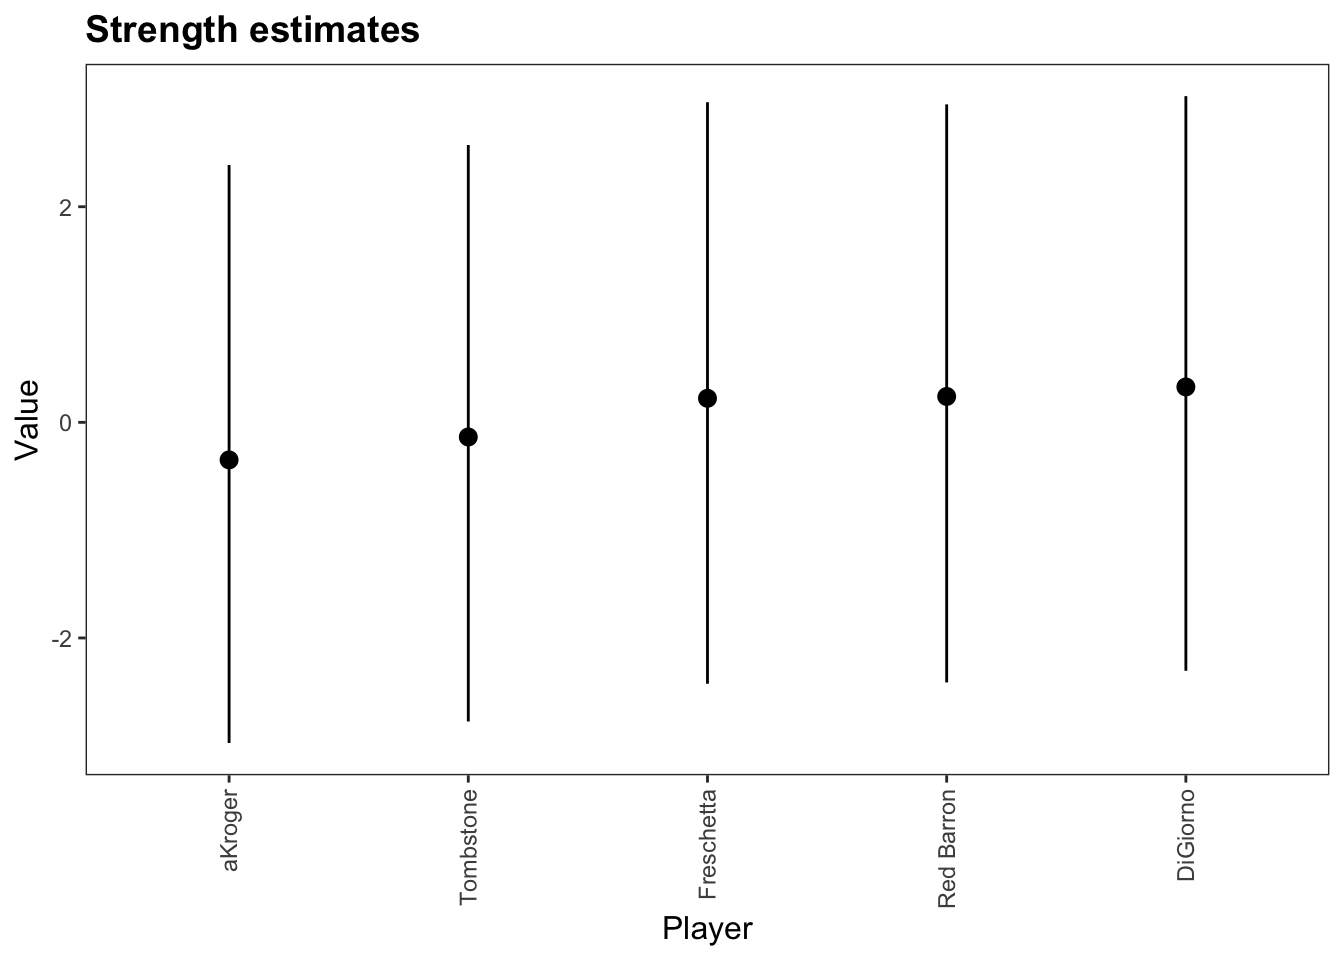
\includegraphics{bpcs-appendix_files/figure-latex/unnamed-chunk-15-1.pdf}

We can also obtain information criteria to compare different models that fit the same data.

Below we show how to obtain the WAIC

\begin{Shaded}
\begin{Highlighting}[]
\KeywordTok{get_waic}\NormalTok{(m)}
\end{Highlighting}
\end{Shaded}

\begin{verbatim}
## 
## Computed from 8000 by 380 log-likelihood matrix
## 
##           Estimate  SE
## elpd_waic   -259.8 3.9
## p_waic         4.0 0.1
## waic         519.6 7.8
\end{verbatim}

This chapter show some basic functionality of the package. The next chapters will show how to apply these functions to solve more interesting and complex problems. We also recommend checking the package documentation at: \url{https://davidissamattos.github.io/bpcs/index.html}

\hypertarget{studyI}{%
\chapter{Re-analysis 1}\label{studyI}}

This reanalysis is based on the paper:

\begin{quote}
Iwasa, Kazunori, et al.~``Visual perception of moisture is a pathogen detection mechanism of the behavioral immune system.'' Frontiers in Psychology 11 (2020): 170.
\end{quote}

The data of this paper can be obtained from the repository: \url{https://osf.io/5quj9/}

\begin{Shaded}
\begin{Highlighting}[]
\KeywordTok{library}\NormalTok{(bpcs)}
\KeywordTok{library}\NormalTok{(tidyverse)}
\KeywordTok{options}\NormalTok{(}\DataTypeTok{mc.cores =}\NormalTok{ parallel}\OperatorTok{::}\KeywordTok{detectCores}\NormalTok{())}
\NormalTok{rstan}\OperatorTok{::}\KeywordTok{rstan_options}\NormalTok{(}\DataTypeTok{auto_write =} \OtherTok{TRUE}\NormalTok{)}
\KeywordTok{set.seed}\NormalTok{(}\DecValTok{99}\NormalTok{)}
\end{Highlighting}
\end{Shaded}

\hypertarget{importing-the-data}{%
\section{Importing the data}\label{importing-the-data}}

First let's read the data:

\begin{Shaded}
\begin{Highlighting}[]
\NormalTok{d <-}\StringTok{ }\NormalTok{readxl}\OperatorTok{::}\KeywordTok{read_xlsx}\NormalTok{(}\StringTok{'data/moisture.xlsx'}\NormalTok{, }\DataTypeTok{sheet =} \StringTok{'Exp02_BTmodel'}\NormalTok{)}
\end{Highlighting}
\end{Shaded}

Below we show a sample of how the original data looks like:

\begin{Shaded}
\begin{Highlighting}[]
\KeywordTok{sample_n}\NormalTok{(d, }\DataTypeTok{size =} \DecValTok{5}\NormalTok{) }\OperatorTok\StringTok{ }
\StringTok{  }\KeywordTok{kable}\NormalTok{(}\DataTypeTok{caption =} \StringTok{'Sample of the original data'}\NormalTok{) }\OperatorTok\StringTok{ }
\StringTok{  }\NormalTok{kableExtra}\OperatorTok{::}\KeywordTok{scroll_box}\NormalTok{(}\DataTypeTok{width =} \StringTok{"100%"}\NormalTok{)}
\end{Highlighting}
\end{Shaded}

\begin{table}

\caption{\label{tab:unnamed-chunk-19}Sample of the original data}
\centering
\begin{tabular}[t]{l|l|r|r}
\hline
player1 & player2 & win1 & win2\\
\hline
image7 & image6 & 131 & 109\\
\hline
image5 & image6 & 18 & 222\\
\hline
image7 & image2 & 226 & 14\\
\hline
image4 & image1 & 239 & 1\\
\hline
image5 & image8 & 20 & 220\\
\hline
\end{tabular}
\end{table}

The data is in the aggregated format. So let's expand it to the long format

\begin{Shaded}
\begin{Highlighting}[]
\NormalTok{d_moisture <-}\StringTok{ }\KeywordTok{expand_aggregated_data}\NormalTok{(d, }\DataTypeTok{player0 =} \StringTok{'player1'}\NormalTok{, }\DataTypeTok{player1=}\StringTok{'player2'}\NormalTok{, }\DataTypeTok{wins0 =} \StringTok{'win1'}\NormalTok{, }\DataTypeTok{wins1=}\StringTok{'win2'}\NormalTok{)}
\end{Highlighting}
\end{Shaded}

Now the data looks like this:

\begin{Shaded}
\begin{Highlighting}[]
\KeywordTok{sample_n}\NormalTok{(d_moisture, }\DataTypeTok{size =} \DecValTok{20}\NormalTok{) }\OperatorTok\StringTok{ }
\StringTok{  }\KeywordTok{kable}\NormalTok{(}\DataTypeTok{caption =} \StringTok{'The data in the long format'}\NormalTok{) }\OperatorTok\StringTok{ }
\StringTok{  }\NormalTok{kableExtra}\OperatorTok{::}\KeywordTok{scroll_box}\NormalTok{(}\DataTypeTok{width =} \StringTok{"100%"}\NormalTok{)}
\end{Highlighting}
\end{Shaded}

\begin{table}

\caption{\label{tab:unnamed-chunk-20}The data in the long format}
\centering
\begin{tabular}[t]{l|l|r|r}
\hline
player0 & player1 & y & rowid\\
\hline
image2 & image7 & 1 & 2922\\
\hline
image5 & image2 & 0 & 7102\\
\hline
image7 & image6 & 1 & 11490\\
\hline
image2 & image8 & 1 & 3200\\
\hline
image1 & image3 & 1 & 358\\
\hline
image8 & image4 & 1 & 12704\\
\hline
image6 & image3 & 0 & 8973\\
\hline
image8 & image3 & 0 & 12308\\
\hline
image6 & image4 & 0 & 9188\\
\hline
image5 & image2 & 0 & 7071\\
\hline
image5 & image1 & 0 & 6724\\
\hline
image4 & image7 & 1 & 6409\\
\hline
image8 & image1 & 0 & 11986\\
\hline
image4 & image1 & 0 & 5278\\
\hline
image3 & image7 & 1 & 4694\\
\hline
image4 & image5 & 1 & 5972\\
\hline
image1 & image8 & 1 & 1533\\
\hline
image4 & image8 & 1 & 6560\\
\hline
image1 & image3 & 1 & 398\\
\hline
image3 & image5 & 1 & 4228\\
\hline
\end{tabular}
\end{table}

\hypertarget{analysis-with-the-bradley-terry-model-and-the-order-effect-model}{%
\section{Analysis with the Bradley-Terry model and the order effect model}\label{analysis-with-the-bradley-terry-model-and-the-order-effect-model}}

Although this is multiple judgment case, the dataset in the aggregated format does not provide information of how each individual voted, therefore we cannot compensate this effect. Therefore, we will create an analysis with only the Bradley-Terry model and the Bradley-Terry model with order effect

First, let's sample the Bradley-Terry model

\begin{Shaded}
\begin{Highlighting}[]
\NormalTok{m_moisture <-}
\StringTok{  }\KeywordTok{bpc}\NormalTok{(}
\NormalTok{    d_moisture,}
    \DataTypeTok{player0 =} \StringTok{'player0'}\NormalTok{,}
    \DataTypeTok{player1 =} \StringTok{'player1'}\NormalTok{,}
    \DataTypeTok{result_column =} \StringTok{'y'}\NormalTok{,}
    \DataTypeTok{model_type =} \StringTok{'bt'}\NormalTok{,}
    \DataTypeTok{iter =} \DecValTok{3000}
\NormalTok{  )}
\KeywordTok{save_bpc_model}\NormalTok{(m_moisture,}\StringTok{'m_moisture'}\NormalTok{,}\StringTok{'fittedmodels'}\NormalTok{)}
\end{Highlighting}
\end{Shaded}

Low let's sample the model with order effect.

Although the authors said that the order of the images was inverted to compensate order effect, we can still estimate if there is an order effect or not in the choice.

But first we need to create a column indicating if there was order effect for that case or not. In this problem, we just indicate with a column of ones that all instances could have an order effect. Not that the package marks the order effect relative to player1. So if the values should be interpret as such.

\begin{Shaded}
\begin{Highlighting}[]
\NormalTok{d_moisture <-}\StringTok{ }\NormalTok{d_moisture }\OperatorTok\StringTok{ }
\StringTok{  }\NormalTok{dplyr}\OperatorTok{::}\KeywordTok{mutate}\NormalTok{(}\DataTypeTok{z1 =} \DecValTok{1}\NormalTok{)}
\end{Highlighting}
\end{Shaded}

\begin{Shaded}
\begin{Highlighting}[]
\NormalTok{m_moisture_order <-}
\StringTok{  }\KeywordTok{bpc}\NormalTok{(}
\NormalTok{    d_moisture,}
    \DataTypeTok{player0 =} \StringTok{'player0'}\NormalTok{,}
    \DataTypeTok{player1 =} \StringTok{'player1'}\NormalTok{,}
    \DataTypeTok{result_column =} \StringTok{'y'}\NormalTok{,}
    \DataTypeTok{z_player1 =} \StringTok{'z1'}\NormalTok{,}
    \DataTypeTok{model_type =} \StringTok{'bt-ordereffect'}\NormalTok{,}
    \DataTypeTok{iter =} \DecValTok{3000}
\NormalTok{  )}
\KeywordTok{save_bpc_model}\NormalTok{(m_moisture_order,}\StringTok{'m_moisture_order'}\NormalTok{,}\StringTok{'fittedmodels'}\NormalTok{)}
\end{Highlighting}
\end{Shaded}

\hypertarget{diagnostics-1}{%
\section{Diagnostics}\label{diagnostics-1}}

Checking convergence of the models

\begin{Shaded}
\begin{Highlighting}[]
\KeywordTok{launch_shinystan}\NormalTok{(m_moisture)}
\end{Highlighting}
\end{Shaded}

\begin{Shaded}
\begin{Highlighting}[]
\KeywordTok{launch_shinystan}\NormalTok{(m_moisture_order)}
\end{Highlighting}
\end{Shaded}

\hypertarget{tables-and-plots}{%
\subsection{Tables and plots}\label{tables-and-plots}}

First, lets get a table for the parameters (to export it to Latex just utilize the format option)

\begin{Shaded}
\begin{Highlighting}[]
\KeywordTok{get_parameters_table}\NormalTok{(m_moisture, }\DataTypeTok{format =} \StringTok{'html'}\NormalTok{, }\DataTypeTok{caption =} \StringTok{'Parameters estimates for the simple Bradley-Terry model'}\NormalTok{)}
\end{Highlighting}
\end{Shaded}

\label{tab:unnamed-chunk-27}Parameters estimates for the simple Bradley-Terry model

Parameter

Mean

HPD\_lower

HPD\_higher

lambda{[}image1{]}

-4.461

-6.507

-2.307

lambda{[}image2{]}

-2.350

-4.459

-0.257

lambda{[}image3{]}

-0.038

-2.138

2.061

lambda{[}image4{]}

0.153

-1.933

2.273

lambda{[}image5{]}

0.313

-1.805

2.377

lambda{[}image6{]}

1.855

-0.243

3.974

lambda{[}image7{]}

2.032

-0.069

4.128

lambda{[}image8{]}

3.044

0.849

5.060

\begin{Shaded}
\begin{Highlighting}[]
\KeywordTok{get_parameters_table}\NormalTok{(}
\NormalTok{  m_moisture_order,}
  \DataTypeTok{params =} \KeywordTok{c}\NormalTok{(}\StringTok{'lambda'}\NormalTok{, }\StringTok{'gm'}\NormalTok{),}
  \DataTypeTok{format =} \StringTok{'html'}\NormalTok{,}
  \DataTypeTok{caption =} \StringTok{'Parameters estimates for the Bradley-Terry model with order effect'}
\NormalTok{)}
\end{Highlighting}
\end{Shaded}

\label{tab:unnamed-chunk-28}Parameters estimates for the Bradley-Terry model with order effect

Parameter

Mean

HPD\_lower

HPD\_higher

lambda{[}image1{]}

-4.524

-6.526

-2.428

lambda{[}image2{]}

-2.410

-4.338

-0.281

lambda{[}image3{]}

-0.097

-2.029

2.020

lambda{[}image4{]}

0.095

-1.834

2.226

lambda{[}image5{]}

0.254

-1.679

2.377

lambda{[}image6{]}

1.799

-0.107

3.955

lambda{[}image7{]}

1.974

0.017

4.083

lambda{[}image8{]}

2.988

1.026

5.100

gm

0.001

-0.054

0.057

We can see from the table of the order effect that the gamma parameter is very close to zero, indicating that there is no order effect

Now lets compute the posterior ranks of the images based on the first BT model

\begin{Shaded}
\begin{Highlighting}[]
\NormalTok{r <-}\StringTok{ }\KeywordTok{get_rank_of_players_df}\NormalTok{(m_moisture) }
\end{Highlighting}
\end{Shaded}

Generating a table with the images

\begin{Shaded}
\begin{Highlighting}[]
\NormalTok{r }\OperatorTok\StringTok{ }
\StringTok{  }\KeywordTok{mutate}\NormalTok{(}\DataTypeTok{Image =} \KeywordTok{c}\NormalTok{(}\StringTok{"data/moisture/Stimuli/image08.jpg"}\NormalTok{,}
                   \StringTok{"data/moisture/Stimuli/image07.jpg"}\NormalTok{,}
                   \StringTok{"data/moisture/Stimuli/image06.jpg"}\NormalTok{,}
                   \StringTok{"data/moisture/Stimuli/image05.jpg"}\NormalTok{,}
                   \StringTok{"data/moisture/Stimuli/image04.jpg"}\NormalTok{,}
                   \StringTok{"data/moisture/Stimuli/image03.jpg"}\NormalTok{,}
                   \StringTok{"data/moisture/Stimuli/image02.jpg"}\NormalTok{,}
                   \StringTok{"data/moisture/Stimuli/image01.jpg"}\NormalTok{) }\OperatorTok\StringTok{ }\NormalTok{pander}\OperatorTok{::}\KeywordTok{pandoc.image.return}\NormalTok{()) }\OperatorTok\StringTok{ }
\StringTok{  }\NormalTok{knitr}\OperatorTok{::}\KeywordTok{kable}\NormalTok{(}\DataTypeTok{caption =} \StringTok{"Rank of the images based on moisture content"}\NormalTok{, }\DataTypeTok{format=}\StringTok{'html'}\NormalTok{, }\DataTypeTok{booktabs=}\NormalTok{T)}
\end{Highlighting}
\end{Shaded}

\label{tab:unnamed-chunk-32}Rank of the images based on moisture content

Parameter

MedianRank

MeanRank

StdRank

Image

lambda{[}image8{]}

1

1.000

0.0000000


\includegraphics{data/moisture/Stimuli/image08.jpg}

lambda{[}image7{]}

2

2.003

0.0547174

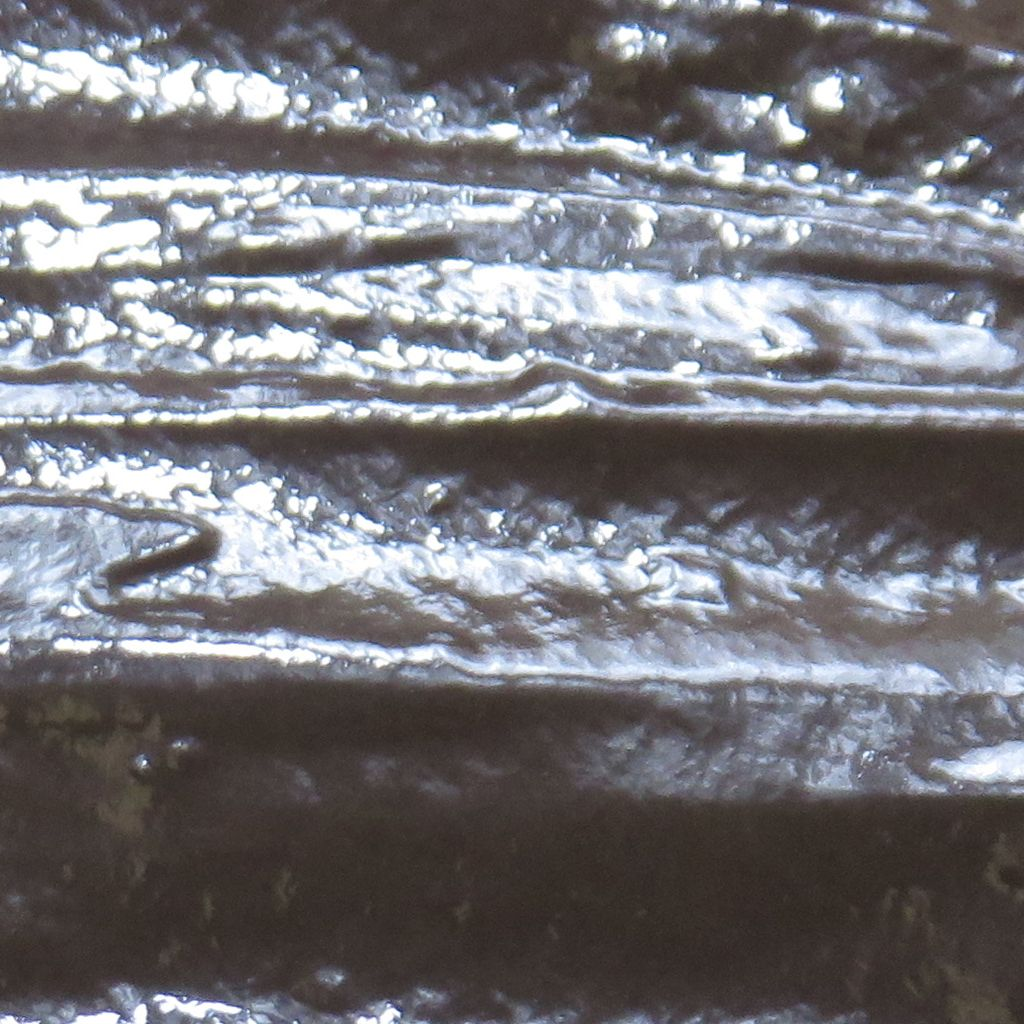
\includegraphics{data/moisture/Stimuli/image07.jpg}

lambda{[}image6{]}

3

2.997

0.0547174

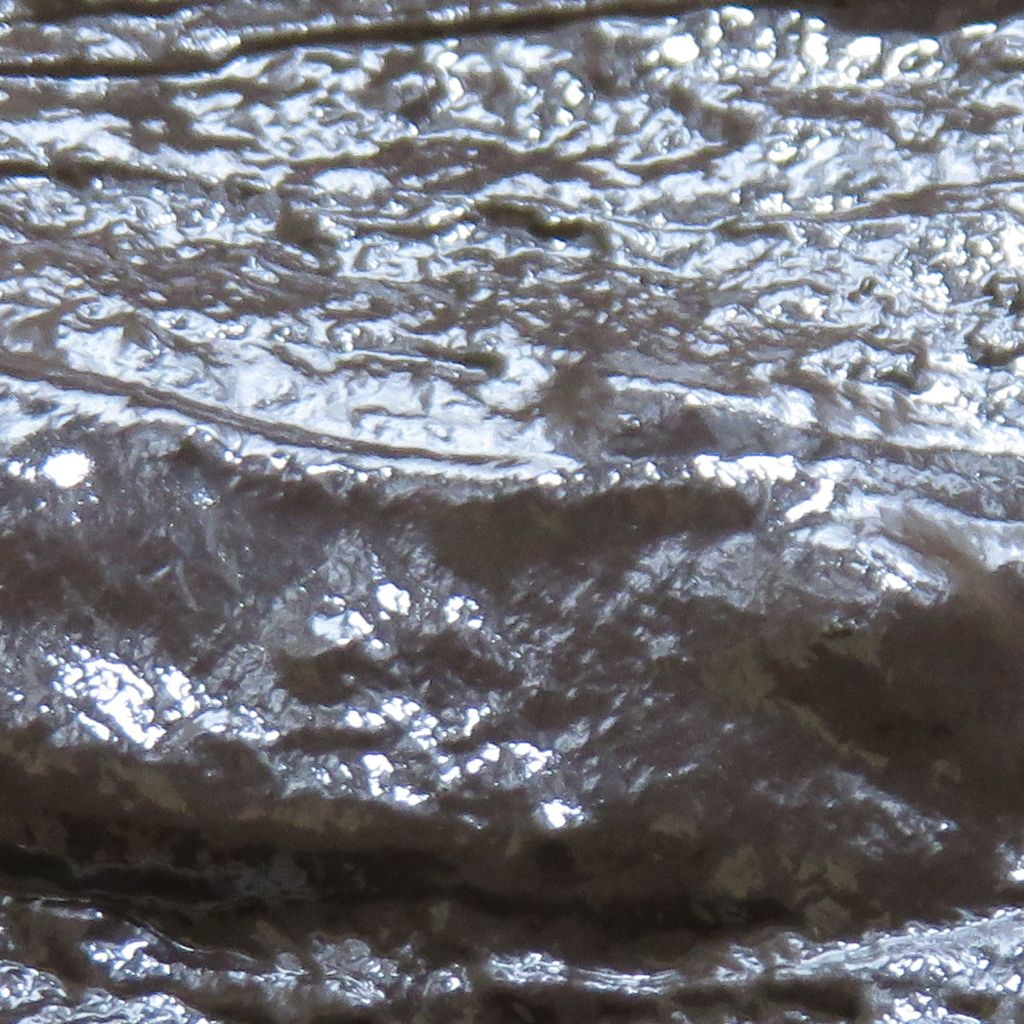
\includegraphics{data/moisture/Stimuli/image06.jpg}

lambda{[}image5{]}

4

4.008

0.0891288

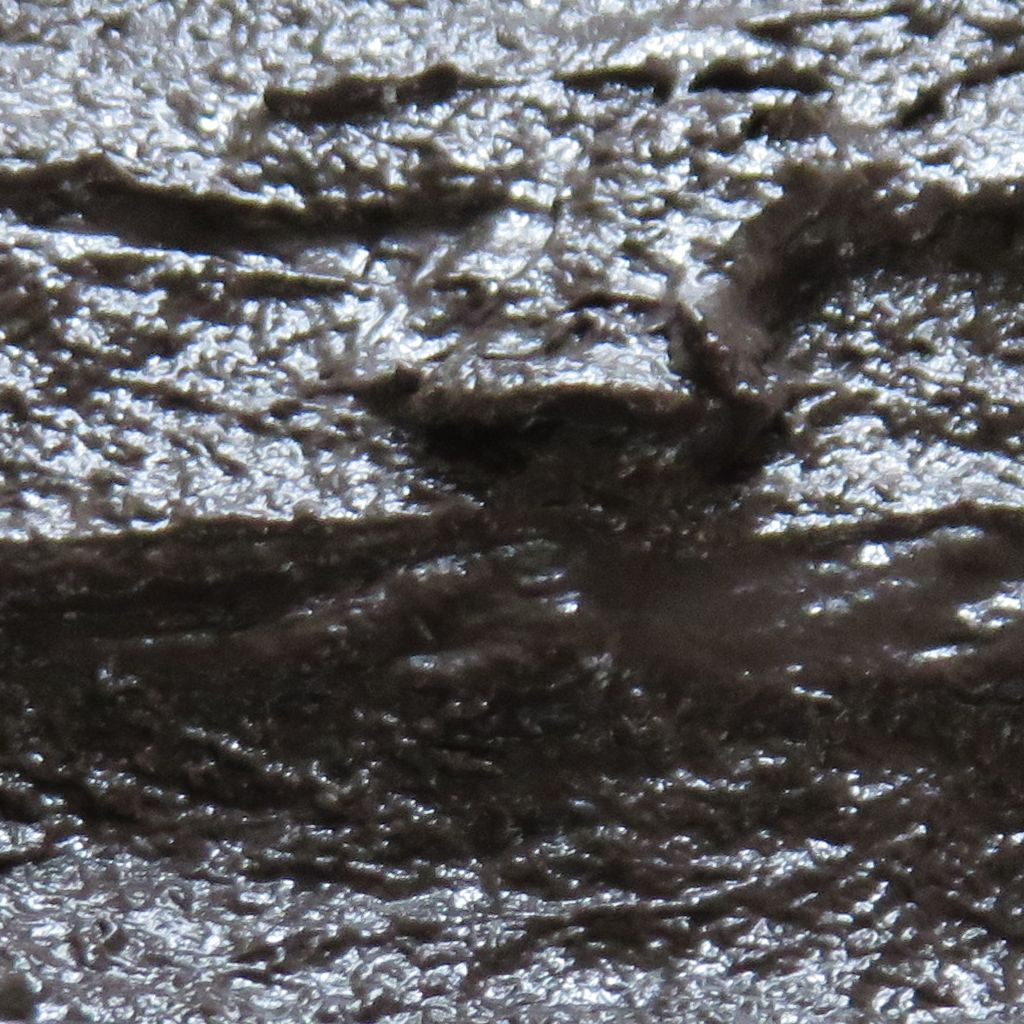
\includegraphics{data/moisture/Stimuli/image05.jpg}

lambda{[}image4{]}

5

4.993

0.0946571

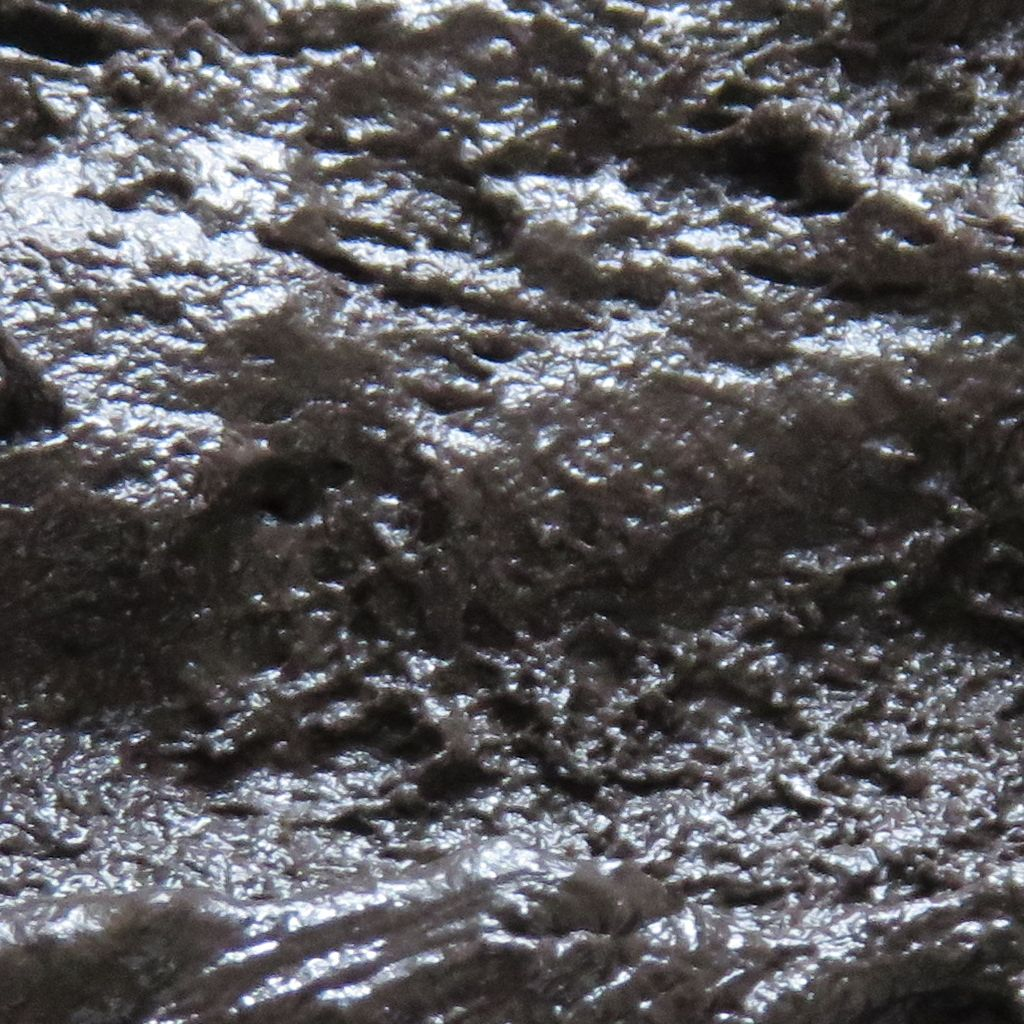
\includegraphics{data/moisture/Stimuli/image04.jpg}

lambda{[}image3{]}

6

5.999

0.0316228

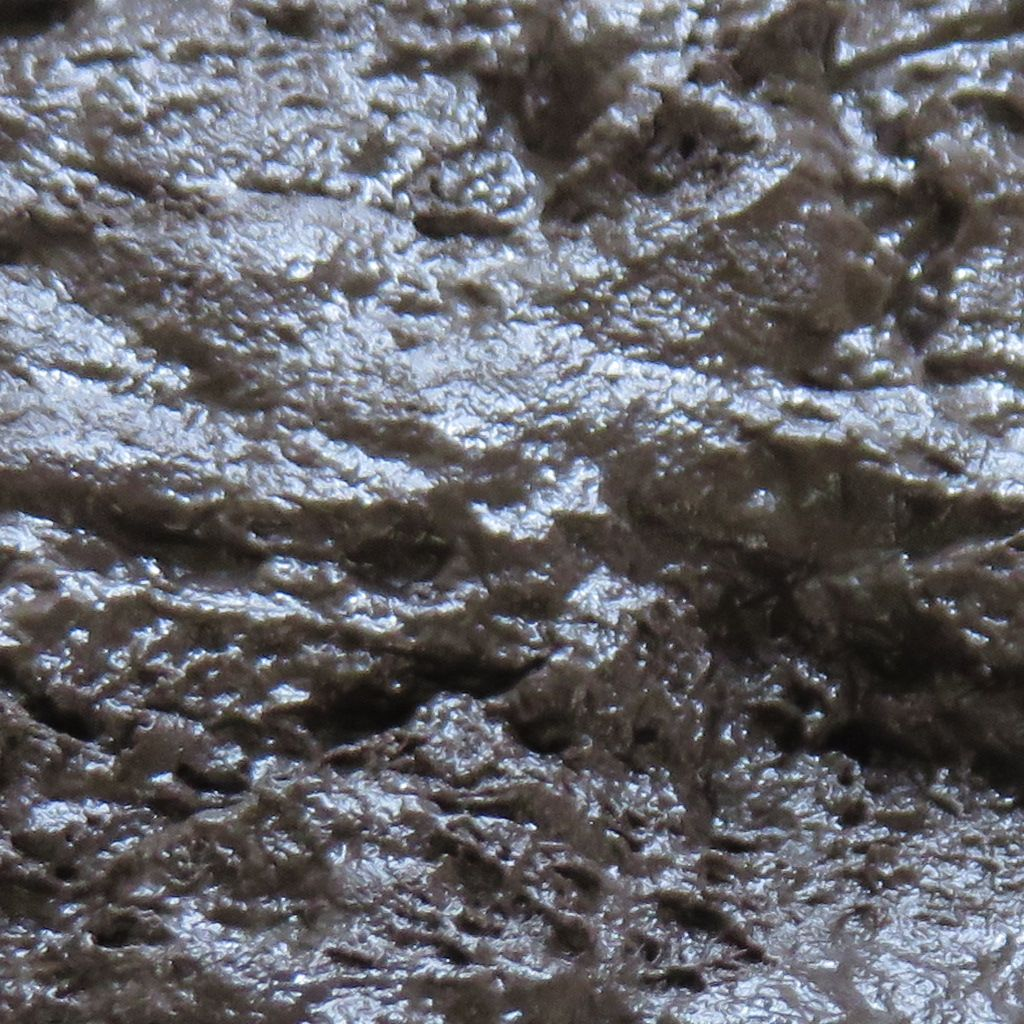
\includegraphics{data/moisture/Stimuli/image03.jpg}

lambda{[}image2{]}

7

7.000

0.0000000

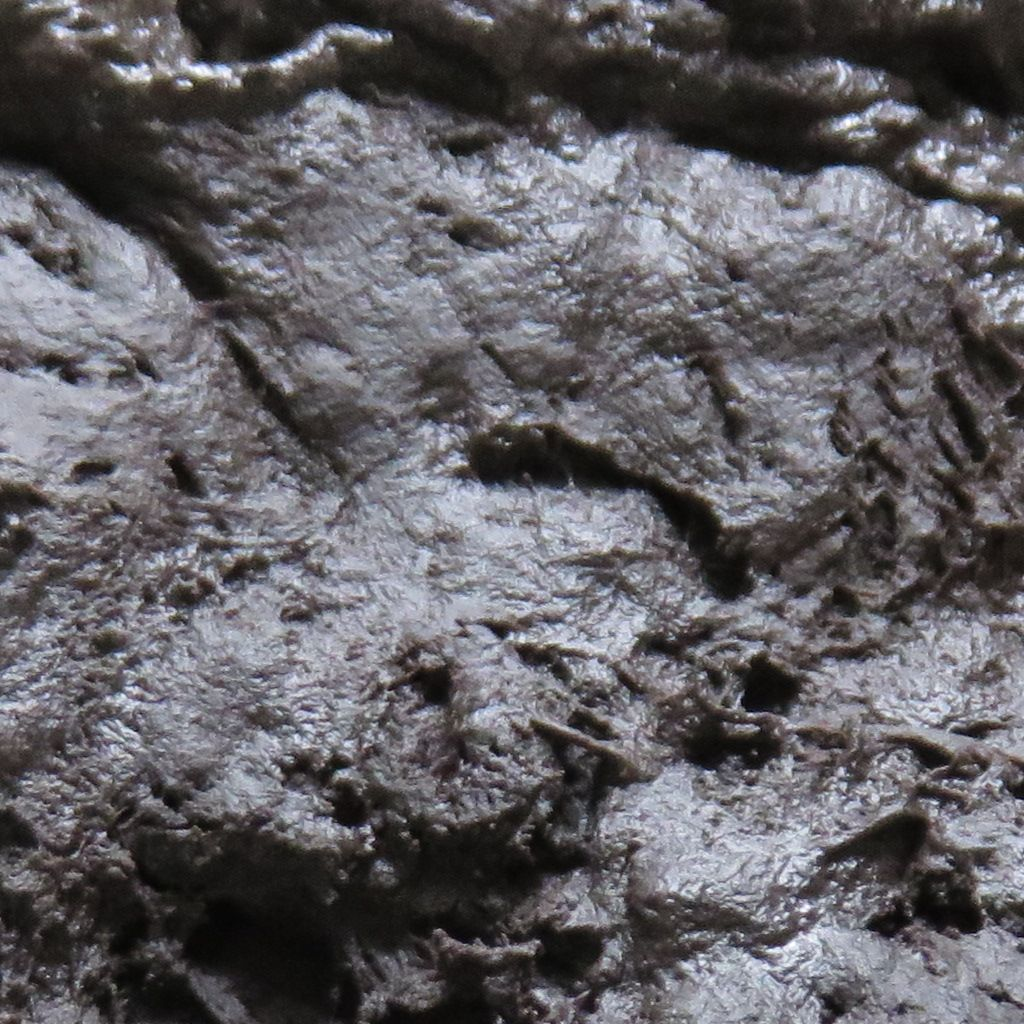
\includegraphics{data/moisture/Stimuli/image02.jpg}

lambda{[}image1{]}

8

8.000

0.0000000

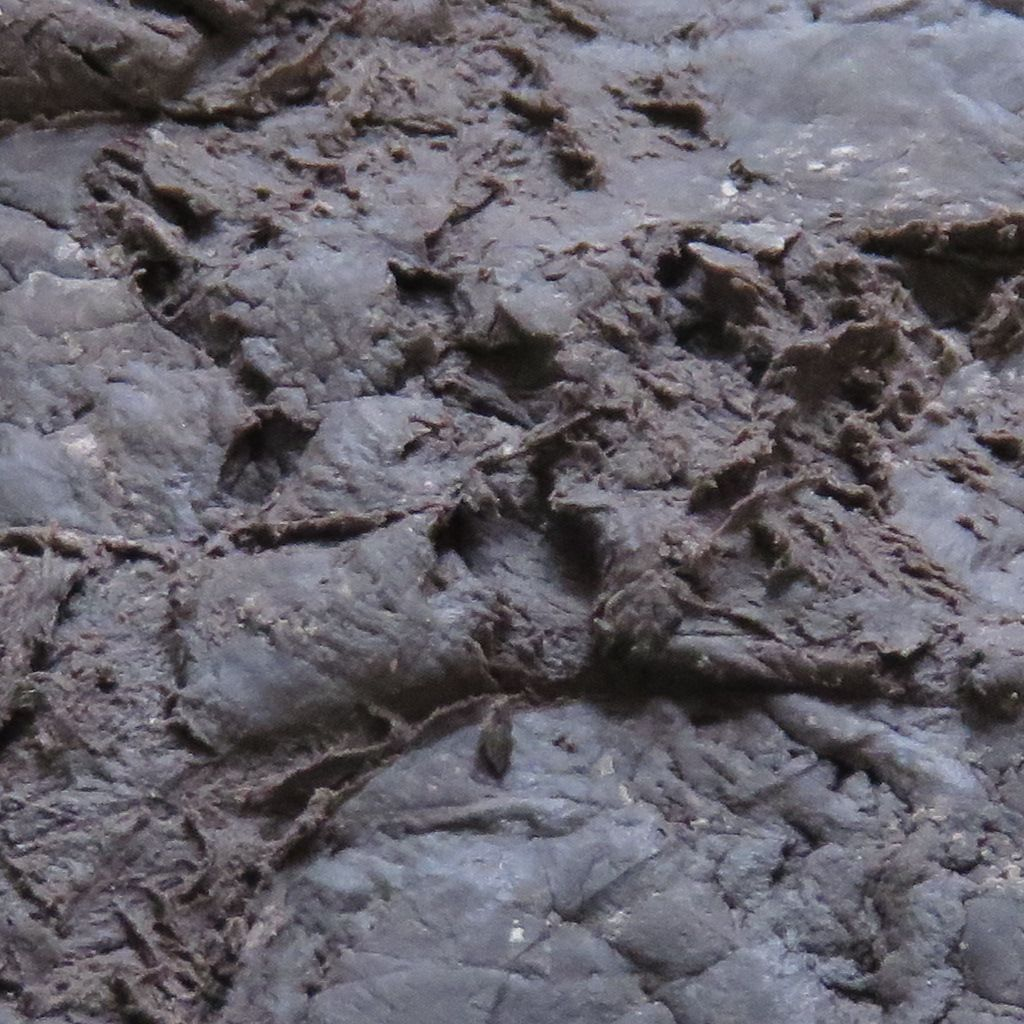
\includegraphics{data/moisture/Stimuli/image01.jpg}

Now lets get a caterpillar style plot

\begin{Shaded}
\begin{Highlighting}[]
\KeywordTok{get_parameters_plot}\NormalTok{(}
\NormalTok{  m_moisture,}
  \DataTypeTok{HPDI =}\NormalTok{ T,}
  \DataTypeTok{title =} \StringTok{'Estimates of the moisture content'}\NormalTok{,}
  \DataTypeTok{xaxis =} \StringTok{'Images'}\NormalTok{,}
  \DataTypeTok{yaxis =} \StringTok{'Ability'}\NormalTok{,}
  \DataTypeTok{rotate_x_labels =}\NormalTok{ F,}
  \DataTypeTok{APA =}\NormalTok{ F}
\NormalTok{) }\OperatorTok{+}\StringTok{ }\KeywordTok{scale_x_discrete}\NormalTok{(}
  \DataTypeTok{labels =} \KeywordTok{c}\NormalTok{(}
    \StringTok{"image1"}\NormalTok{,}
    \StringTok{"image2"}\NormalTok{,}
    \StringTok{"image3"}\NormalTok{,}
    \StringTok{"image4"}\NormalTok{,}
    \StringTok{"image5"}\NormalTok{,}
    \StringTok{"image6"}\NormalTok{,}
    \StringTok{"image7"}\NormalTok{,}
    \StringTok{"image8"}
\NormalTok{  )}
\NormalTok{) }\OperatorTok{+}\StringTok{ }\KeywordTok{theme_bw}\NormalTok{()}
\end{Highlighting}
\end{Shaded}

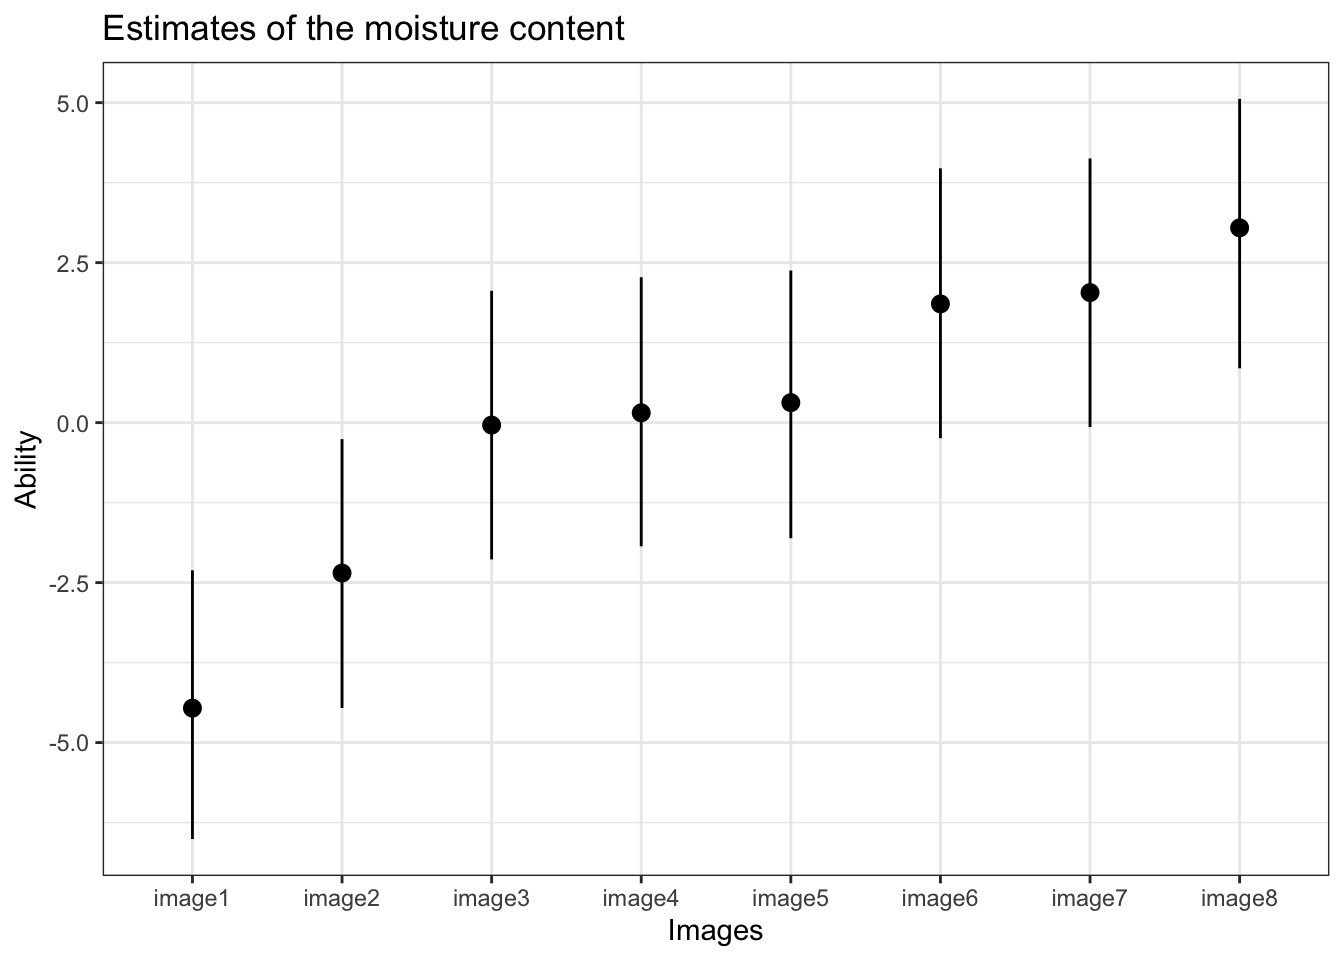
\includegraphics{bpcs-appendix_files/figure-latex/unnamed-chunk-33-1.pdf}

\hypertarget{waic}{%
\subsection{WAIC}\label{waic}}

Calculating the WAIC of both models

\begin{Shaded}
\begin{Highlighting}[]
\KeywordTok{get_waic}\NormalTok{(m_moisture)}
\end{Highlighting}
\end{Shaded}

\begin{verbatim}
## 
## Computed from 8000 by 13440 log-likelihood matrix
## 
##           Estimate    SE
## elpd_waic  -4066.1  78.8
## p_waic         6.9   0.2
## waic        8132.2 157.6
\end{verbatim}

\begin{Shaded}
\begin{Highlighting}[]
\KeywordTok{get_waic}\NormalTok{(m_moisture_order)}
\end{Highlighting}
\end{Shaded}

\begin{verbatim}
## 
## Computed from 8000 by 13440 log-likelihood matrix
## 
##           Estimate    SE
## elpd_waic  -4067.1  78.9
## p_waic         7.8   0.2
## waic        8134.2 157.7
\end{verbatim}

We can see that the WAIC of the models are quite similar and that the model without the order effect has a slightly smaller WAIC and less parameters. Therefore we will select it.

\hypertarget{studyII}{%
\chapter{Re-analysis 2}\label{studyII}}

This reanalysis is based on the paper:

\begin{quote}
Huskisson, S.M., Jacobson, S.L., Egelkamp, C.L. et al.~Using a Touchscreen Paradigm to Evaluate Food Preferences and Response to Novel Photographic Stimuli of Food in Three Primate Species (Gorilla gorilla gorilla, Pan troglodytes, and Macaca fuscata). Int J Primatol 41, 5--23 (2020). \url{https://doi.org/10.1007/s10764-020-00131-0}
\end{quote}

\begin{Shaded}
\begin{Highlighting}[]
\KeywordTok{library}\NormalTok{(bpcs)}
\KeywordTok{library}\NormalTok{(tidyverse)}
\KeywordTok{library}\NormalTok{(knitr)}
\KeywordTok{options}\NormalTok{(}\DataTypeTok{mc.cores =}\NormalTok{ parallel}\OperatorTok{::}\KeywordTok{detectCores}\NormalTok{())}
\NormalTok{rstan}\OperatorTok{::}\KeywordTok{rstan_options}\NormalTok{(}\DataTypeTok{auto_write =} \OtherTok{TRUE}\NormalTok{)}
\KeywordTok{set.seed}\NormalTok{(}\DecValTok{99}\NormalTok{)}
\end{Highlighting}
\end{Shaded}

\hypertarget{importing-the-data-1}{%
\section{Importing the data}\label{importing-the-data-1}}

The data from this paper was made available upon request and below we exemplify a few rows of how the original dataset looks like

\begin{Shaded}
\begin{Highlighting}[]
\NormalTok{d <-}\StringTok{ }\NormalTok{readr}\OperatorTok{::}\KeywordTok{read_csv}\NormalTok{(}\StringTok{'data/touchscreen.csv'}\NormalTok{)}
\end{Highlighting}
\end{Shaded}

Previewing how the data looks like

\begin{Shaded}
\begin{Highlighting}[]
\NormalTok{dplyr}\OperatorTok{::}\KeywordTok{sample_n}\NormalTok{(d, }\DataTypeTok{size =} \DecValTok{10}\NormalTok{) }\OperatorTok\StringTok{ }
\StringTok{  }\NormalTok{knitr}\OperatorTok{::}\KeywordTok{kable}\NormalTok{(}\DataTypeTok{caption=}\StringTok{'Sample of how the dataset looks like'}\NormalTok{) }\OperatorTok\StringTok{ }
\StringTok{  }\NormalTok{kableExtra}\OperatorTok{::}\KeywordTok{kable_styling}\NormalTok{(}\DataTypeTok{bootstrap_options =} \KeywordTok{c}\NormalTok{(}\StringTok{"striped"}\NormalTok{, }\StringTok{"hover"}\NormalTok{, }\StringTok{"condensed"}\NormalTok{, }\StringTok{"responsive"}\NormalTok{)) }\OperatorTok\StringTok{ }
\StringTok{  }\NormalTok{kableExtra}\OperatorTok{::}\KeywordTok{scroll_box}\NormalTok{(}\DataTypeTok{width =} \StringTok{"100%"}\NormalTok{)}
\end{Highlighting}
\end{Shaded}

\begin{table}

\caption{\label{tab:unnamed-chunk-38}Sample of how the dataset looks like}
\centering
\begin{tabular}[t]{l|l|l|l|r|l|l|l|l}
\hline
date & species\_type & SubjectCode & Sex & Trial & image1 & image2 & image\_chosen & concat\_test\_name\\
\hline
10/12/17 & Gorilla & Gorilla1 & Male & 2 & Ap & Cu & Ap & ApCu\\
\hline
8/31/17 & Gorilla & Gorilla3 & Male & 16 & Ca & To & To & CaTo\\
\hline
8/16/17 & Gorilla & Gorilla5 & Female & 16 & Cu & Gr & Cu & CuGr\\
\hline
11/13/17 & Chimpanzee & Chimpanzee3 & Female & 14 & Ap & Ca & Ca & ApCa\\
\hline
4/11/17 & Gorilla & Gorilla3 & Male & 15 & Ca & Cu & Ca & CaCu\\
\hline
1/22/18 & Macaque & Macaque7 & Female & 1 & Ca & Pe & Pe & CaPe\\
\hline
1/5/17 & Gorilla & Gorilla4 & Male & 28 & Ca & Tu & Tu & CaTu\\
\hline
3/3/17 & Chimpanzee & Chimpanzee1 & Female & 19 & Cu & Gr & Gr & CuGr\\
\hline
12/4/17 & Chimpanzee & Chimpanzee1 & Female & 27 & Ap & Tu & Tu & ApTu\\
\hline
5/1/17 & Gorilla & Gorilla6 & Male & 14 & Ca & Tu & Ca & CaTu\\
\hline
\end{tabular}
\end{table}

Now we need to modify a bit the data frame to create a column with the results as 0 and 1.

Creating a numerical result vector with 0 for image1 and 1 for image2

\begin{Shaded}
\begin{Highlighting}[]
\NormalTok{d <-}\StringTok{ }\NormalTok{d }\OperatorTok\StringTok{ }
\StringTok{  }\NormalTok{dplyr}\OperatorTok{::}\KeywordTok{mutate}\NormalTok{(}\DataTypeTok{y =}\KeywordTok{ifelse}\NormalTok{(image_chosen}\OperatorTok{==}\NormalTok{image1, }\DecValTok{0}\NormalTok{, }\DecValTok{1}\NormalTok{))}
\end{Highlighting}
\end{Shaded}

Adding names to the abbreviations

\begin{Shaded}
\begin{Highlighting}[]
\CommentTok{#image1}
\NormalTok{d}\OperatorTok{$}\NormalTok{image1 <-}\StringTok{ }\NormalTok{dplyr}\OperatorTok{::}\KeywordTok{recode}\NormalTok{(d}\OperatorTok{$}\NormalTok{image1, }\StringTok{"Ca"}\NormalTok{ =}\StringTok{ 'Carrot'}\NormalTok{)}
\NormalTok{d}\OperatorTok{$}\NormalTok{image1 <-}\StringTok{ }\NormalTok{dplyr}\OperatorTok{::}\KeywordTok{recode}\NormalTok{(d}\OperatorTok{$}\NormalTok{image1, }\StringTok{"Cu"}\NormalTok{ =}\StringTok{ 'Cucumber'}\NormalTok{)}
\NormalTok{d}\OperatorTok{$}\NormalTok{image1 <-}\StringTok{ }\NormalTok{dplyr}\OperatorTok{::}\KeywordTok{recode}\NormalTok{(d}\OperatorTok{$}\NormalTok{image1, }\StringTok{"Tu"}\NormalTok{ =}\StringTok{ 'Turnip'}\NormalTok{)}
\NormalTok{d}\OperatorTok{$}\NormalTok{image1 <-}\StringTok{ }\NormalTok{dplyr}\OperatorTok{::}\KeywordTok{recode}\NormalTok{(d}\OperatorTok{$}\NormalTok{image1, }\StringTok{"Gr"}\NormalTok{ =}\StringTok{ 'Grape'}\NormalTok{)}
\NormalTok{d}\OperatorTok{$}\NormalTok{image1 <-}\StringTok{ }\NormalTok{dplyr}\OperatorTok{::}\KeywordTok{recode}\NormalTok{(d}\OperatorTok{$}\NormalTok{image1, }\StringTok{"To"}\NormalTok{ =}\StringTok{ 'Tomato'}\NormalTok{)}
\NormalTok{d}\OperatorTok{$}\NormalTok{image1 <-}\StringTok{ }\NormalTok{dplyr}\OperatorTok{::}\KeywordTok{recode}\NormalTok{(d}\OperatorTok{$}\NormalTok{image1, }\StringTok{"Ap"}\NormalTok{ =}\StringTok{ 'Apple'}\NormalTok{)}
\NormalTok{d}\OperatorTok{$}\NormalTok{image1 <-}\StringTok{ }\NormalTok{dplyr}\OperatorTok{::}\KeywordTok{recode}\NormalTok{(d}\OperatorTok{$}\NormalTok{image1, }\StringTok{"Jp"}\NormalTok{ =}\StringTok{ 'Jungle Pellet'}\NormalTok{)}
\NormalTok{d}\OperatorTok{$}\NormalTok{image1 <-}\StringTok{ }\NormalTok{dplyr}\OperatorTok{::}\KeywordTok{recode}\NormalTok{(d}\OperatorTok{$}\NormalTok{image1, }\StringTok{"Ce"}\NormalTok{ =}\StringTok{ 'Celery'}\NormalTok{)}
\NormalTok{d}\OperatorTok{$}\NormalTok{image1 <-}\StringTok{ }\NormalTok{dplyr}\OperatorTok{::}\KeywordTok{recode}\NormalTok{(d}\OperatorTok{$}\NormalTok{image1, }\StringTok{"Gb"}\NormalTok{ =}\StringTok{ 'Green Beans'}\NormalTok{)}
\NormalTok{d}\OperatorTok{$}\NormalTok{image1 <-}\StringTok{ }\NormalTok{dplyr}\OperatorTok{::}\KeywordTok{recode}\NormalTok{(d}\OperatorTok{$}\NormalTok{image1, }\StringTok{"Oa"}\NormalTok{ =}\StringTok{ 'Oats'}\NormalTok{)}
\NormalTok{d}\OperatorTok{$}\NormalTok{image1 <-}\StringTok{ }\NormalTok{dplyr}\OperatorTok{::}\KeywordTok{recode}\NormalTok{(d}\OperatorTok{$}\NormalTok{image1, }\StringTok{"Pe"}\NormalTok{ =}\StringTok{ 'Peanuts'}\NormalTok{)}

\CommentTok{#image2}
\NormalTok{d}\OperatorTok{$}\NormalTok{image2 <-}\StringTok{ }\NormalTok{dplyr}\OperatorTok{::}\KeywordTok{recode}\NormalTok{(d}\OperatorTok{$}\NormalTok{image2, }\StringTok{"Ca"}\NormalTok{ =}\StringTok{ 'Carrot'}\NormalTok{)}
\NormalTok{d}\OperatorTok{$}\NormalTok{image2 <-}\StringTok{ }\NormalTok{dplyr}\OperatorTok{::}\KeywordTok{recode}\NormalTok{(d}\OperatorTok{$}\NormalTok{image2, }\StringTok{"Cu"}\NormalTok{ =}\StringTok{ 'Cucumber'}\NormalTok{)}
\NormalTok{d}\OperatorTok{$}\NormalTok{image2 <-}\StringTok{ }\NormalTok{dplyr}\OperatorTok{::}\KeywordTok{recode}\NormalTok{(d}\OperatorTok{$}\NormalTok{image2, }\StringTok{"Tu"}\NormalTok{ =}\StringTok{ 'Turnip'}\NormalTok{)}
\NormalTok{d}\OperatorTok{$}\NormalTok{image2 <-}\StringTok{ }\NormalTok{dplyr}\OperatorTok{::}\KeywordTok{recode}\NormalTok{(d}\OperatorTok{$}\NormalTok{image2, }\StringTok{"Gr"}\NormalTok{ =}\StringTok{ 'Grape'}\NormalTok{)}
\NormalTok{d}\OperatorTok{$}\NormalTok{image2 <-}\StringTok{ }\NormalTok{dplyr}\OperatorTok{::}\KeywordTok{recode}\NormalTok{(d}\OperatorTok{$}\NormalTok{image2, }\StringTok{"To"}\NormalTok{ =}\StringTok{ 'Tomato'}\NormalTok{)}
\NormalTok{d}\OperatorTok{$}\NormalTok{image2 <-}\StringTok{ }\NormalTok{dplyr}\OperatorTok{::}\KeywordTok{recode}\NormalTok{(d}\OperatorTok{$}\NormalTok{image2, }\StringTok{"Ap"}\NormalTok{ =}\StringTok{ 'Apple'}\NormalTok{)}
\NormalTok{d}\OperatorTok{$}\NormalTok{image2 <-}\StringTok{ }\NormalTok{dplyr}\OperatorTok{::}\KeywordTok{recode}\NormalTok{(d}\OperatorTok{$}\NormalTok{image2, }\StringTok{"Jp"}\NormalTok{ =}\StringTok{ 'Jungle Pellet'}\NormalTok{)}
\NormalTok{d}\OperatorTok{$}\NormalTok{image2 <-}\StringTok{ }\NormalTok{dplyr}\OperatorTok{::}\KeywordTok{recode}\NormalTok{(d}\OperatorTok{$}\NormalTok{image2, }\StringTok{"Ce"}\NormalTok{ =}\StringTok{ 'Celery'}\NormalTok{)}
\NormalTok{d}\OperatorTok{$}\NormalTok{image2 <-}\StringTok{ }\NormalTok{dplyr}\OperatorTok{::}\KeywordTok{recode}\NormalTok{(d}\OperatorTok{$}\NormalTok{image2, }\StringTok{"Gb"}\NormalTok{ =}\StringTok{ 'Green Beans'}\NormalTok{)}
\NormalTok{d}\OperatorTok{$}\NormalTok{image2 <-}\StringTok{ }\NormalTok{dplyr}\OperatorTok{::}\KeywordTok{recode}\NormalTok{(d}\OperatorTok{$}\NormalTok{image2, }\StringTok{"Oa"}\NormalTok{ =}\StringTok{ 'Oats'}\NormalTok{)}
\NormalTok{d}\OperatorTok{$}\NormalTok{image2 <-}\StringTok{ }\NormalTok{dplyr}\OperatorTok{::}\KeywordTok{recode}\NormalTok{(d}\OperatorTok{$}\NormalTok{image2, }\StringTok{"Pe"}\NormalTok{ =}\StringTok{ 'Peanuts'}\NormalTok{)}
\end{Highlighting}
\end{Shaded}

Separating the data into three datasets. One for each species.

\begin{Shaded}
\begin{Highlighting}[]
\NormalTok{macaque <-}\StringTok{ }\NormalTok{d }\OperatorTok\StringTok{ }
\StringTok{  }\NormalTok{dplyr}\OperatorTok{::}\KeywordTok{filter}\NormalTok{(species_type}\OperatorTok{==}\StringTok{'Macaque'}\NormalTok{)}

\NormalTok{chip <-}\StringTok{ }\NormalTok{d }\OperatorTok\StringTok{ }
\StringTok{  }\NormalTok{dplyr}\OperatorTok{::}\KeywordTok{filter}\NormalTok{(species_type}\OperatorTok{==}\StringTok{'Chimpanzee'}\NormalTok{)}

\NormalTok{gor <-}\StringTok{ }\NormalTok{d }\OperatorTok\StringTok{ }
\StringTok{  }\NormalTok{dplyr}\OperatorTok{::}\KeywordTok{filter}\NormalTok{(species_type}\OperatorTok{==}\StringTok{'Gorilla'}\NormalTok{)}
\end{Highlighting}
\end{Shaded}

Below we show a few lines of each dataset:

\begin{Shaded}
\begin{Highlighting}[]
\NormalTok{dplyr}\OperatorTok{::}\KeywordTok{sample_n}\NormalTok{(gor, }\DataTypeTok{size =} \DecValTok{10}\NormalTok{) }\OperatorTok\StringTok{ }
\StringTok{  }\NormalTok{knitr}\OperatorTok{::}\KeywordTok{kable}\NormalTok{(}\DataTypeTok{caption=}\StringTok{'Sample of how the gorilla dataset looks like'}\NormalTok{) }\OperatorTok\StringTok{ }
\StringTok{  }\NormalTok{kableExtra}\OperatorTok{::}\KeywordTok{kable_styling}\NormalTok{(}\DataTypeTok{bootstrap_options =} \KeywordTok{c}\NormalTok{(}\StringTok{"striped"}\NormalTok{, }\StringTok{"hover"}\NormalTok{, }\StringTok{"condensed"}\NormalTok{, }\StringTok{"responsive"}\NormalTok{)) }\OperatorTok\StringTok{ }
\StringTok{  }\NormalTok{kableExtra}\OperatorTok{::}\KeywordTok{scroll_box}\NormalTok{(}\DataTypeTok{width =} \StringTok{"100%"}\NormalTok{)}
\end{Highlighting}
\end{Shaded}

\begin{table}

\caption{\label{tab:unnamed-chunk-42}Sample of how the gorilla dataset looks like}
\centering
\begin{tabular}[t]{l|l|l|l|r|l|l|l|l|r}
\hline
date & species\_type & SubjectCode & Sex & Trial & image1 & image2 & image\_chosen & concat\_test\_name & y\\
\hline
3/3/17 & Gorilla & Gorilla2 & Male & 31 & Cucumber & Tomato & To & CuTo & 1\\
\hline
11/8/17 & Gorilla & Gorilla6 & Male & 6 & Tomato & Turnip & To & ToTu & 0\\
\hline
3/20/17 & Gorilla & Gorilla2 & Male & 6 & Grape & Tomato & To & GrTo & 1\\
\hline
3/8/17 & Gorilla & Gorilla6 & Male & 20 & Carrot & Grape & Ca & CaGr & 0\\
\hline
8/23/17 & Gorilla & Gorilla5 & Female & 4 & Cucumber & Grape & Cu & CuGr & 0\\
\hline
5/25/17 & Gorilla & Gorilla4 & Male & 19 & Carrot & Cucumber & Ca & CaCu & 0\\
\hline
8/3/17 & Gorilla & Gorilla6 & Male & 14 & Carrot & Tomato & To & CaTo & 1\\
\hline
8/23/17 & Gorilla & Gorilla5 & Female & 24 & Cucumber & Grape & Gr & CuGr & 1\\
\hline
12/7/16 & Gorilla & Gorilla2 & Male & 28 & Cucumber & Turnip & Cu & CuTu & 0\\
\hline
5/25/17 & Gorilla & Gorilla1 & Male & 4 & Carrot & Cucumber & Ca & CaCu & 0\\
\hline
\end{tabular}
\end{table}

\begin{Shaded}
\begin{Highlighting}[]
\NormalTok{dplyr}\OperatorTok{::}\KeywordTok{sample_n}\NormalTok{(chip, }\DataTypeTok{size =} \DecValTok{10}\NormalTok{) }\OperatorTok\StringTok{ }
\StringTok{  }\NormalTok{knitr}\OperatorTok{::}\KeywordTok{kable}\NormalTok{(}\DataTypeTok{caption=}\StringTok{'Sample of how the chimpanzees dataset looks like'}\NormalTok{) }\OperatorTok\StringTok{ }
\StringTok{  }\NormalTok{kableExtra}\OperatorTok{::}\KeywordTok{kable_styling}\NormalTok{(}\DataTypeTok{bootstrap_options =} \KeywordTok{c}\NormalTok{(}\StringTok{"striped"}\NormalTok{, }\StringTok{"hover"}\NormalTok{, }\StringTok{"condensed"}\NormalTok{, }\StringTok{"responsive"}\NormalTok{)) }\OperatorTok\StringTok{ }
\StringTok{  }\NormalTok{kableExtra}\OperatorTok{::}\KeywordTok{scroll_box}\NormalTok{(}\DataTypeTok{width =} \StringTok{"100%"}\NormalTok{)}
\end{Highlighting}
\end{Shaded}

\begin{table}

\caption{\label{tab:unnamed-chunk-43}Sample of how the chimpanzees dataset looks like}
\centering
\begin{tabular}[t]{l|l|l|l|r|l|l|l|l|r}
\hline
date & species\_type & SubjectCode & Sex & Trial & image1 & image2 & image\_chosen & concat\_test\_name & y\\
\hline
3/1/18 & Chimpanzee & Chimpanzee4 & Male & 3 & Apple & Carrot & Ap & ApCa & 0\\
\hline
12/7/17 & Chimpanzee & Chimpanzee1 & Female & 18 & Carrot & Tomato & To & CaTo & 1\\
\hline
4/26/17 & Chimpanzee & Chimpanzee3 & Female & 7 & Cucumber & Turnip & Cu & CuTu & 0\\
\hline
11/1/17 & Chimpanzee & Chimpanzee1 & Female & 19 & Apple & Grape & Gr & ApGr & 1\\
\hline
7/26/17 & Chimpanzee & Chimpanzee3 & Female & 20 & Cucumber & Grape & Cu & CuGr & 0\\
\hline
10/26/17 & Chimpanzee & Chimpanzee1 & Female & 7 & Apple & Grape & Gr & ApGr & 1\\
\hline
9/18/17 & Chimpanzee & Chimpanzee4 & Male & 27 & Carrot & Grape & Gr & CaGr & 1\\
\hline
12/8/16 & Chimpanzee & Chimpanzee1 & Female & 12 & Cucumber & Turnip & Cu & CuTu & 0\\
\hline
12/14/17 & Chimpanzee & Chimpanzee3 & Female & 14 & Tomato & Turnip & To & ToTu & 0\\
\hline
1/12/17 & Chimpanzee & Chimpanzee4 & Male & 21 & Cucumber & Turnip & Tu & CuTu & 1\\
\hline
\end{tabular}
\end{table}

\begin{Shaded}
\begin{Highlighting}[]
\NormalTok{dplyr}\OperatorTok{::}\KeywordTok{sample_n}\NormalTok{(macaque, }\DataTypeTok{size =} \DecValTok{10}\NormalTok{) }\OperatorTok\StringTok{ }
\StringTok{  }\NormalTok{knitr}\OperatorTok{::}\KeywordTok{kable}\NormalTok{(}\DataTypeTok{caption=}\StringTok{'Sample of how the macaques dataset looks like'}\NormalTok{) }\OperatorTok\StringTok{ }
\StringTok{  }\NormalTok{kableExtra}\OperatorTok{::}\KeywordTok{kable_styling}\NormalTok{(}\DataTypeTok{bootstrap_options =} \KeywordTok{c}\NormalTok{(}\StringTok{"striped"}\NormalTok{, }\StringTok{"hover"}\NormalTok{, }\StringTok{"condensed"}\NormalTok{, }\StringTok{"responsive"}\NormalTok{)) }\OperatorTok\StringTok{ }
\StringTok{  }\NormalTok{kableExtra}\OperatorTok{::}\KeywordTok{scroll_box}\NormalTok{(}\DataTypeTok{width =} \StringTok{"100%"}\NormalTok{)}
\end{Highlighting}
\end{Shaded}

\begin{table}

\caption{\label{tab:unnamed-chunk-44}Sample of how the macaques dataset looks like}
\centering
\begin{tabular}[t]{l|l|l|l|r|l|l|l|l|r}
\hline
date & species\_type & SubjectCode & Sex & Trial & image1 & image2 & image\_chosen & concat\_test\_name & y\\
\hline
10/6/17 & Macaque & Macaque6 & Female & 10 & Jungle Pellet & Celery & Jp & CeJp & 0\\
\hline
09-06-2017@11-43 & Macaque & Macaque1 & Male & 12 & Carrot & Celery & Ca & CeCa & 0\\
\hline
04-30-2018@11-54 & Macaque & Macaque1 & Male & 8 & Peanuts & Oats & Pe & PeOa & 0\\
\hline
8/7/17 & Macaque & Macaque3 & Female & 1 & Peanuts & Celery & Ce & CePe & 1\\
\hline
05-04-2018@11-27 & Macaque & Macaque1 & Male & 1 & Celery & Green Beans & Gb & GbCe & 1\\
\hline
1/16/18 & Macaque & Macaque7 & Female & 14 & Carrot & Peanuts & Ca & CaPe & 0\\
\hline
04-02-2018@11-27 & Macaque & Macaque1 & Male & 28 & Carrot & Green Beans & Ca & GbCa & 0\\
\hline
9/7/17 & Macaque & Macaque6 & Female & 2 & Carrot & Celery & Ca & CeCa & 0\\
\hline
8/14/17 & Macaque & Macaque2 & Female & 14 & Carrot & Peanuts & Pe & CaPe & 1\\
\hline
5/24/18 & Macaque & Macaque4 & Female & 17 & Jungle Pellet & Oats & Jp & JpOa & 0\\
\hline
\end{tabular}
\end{table}

\hypertarget{simple-bradley-terry-model}{%
\section{Simple Bradley-Terry model}\label{simple-bradley-terry-model}}

Now that the data is ready let's fit three simple Bayesian Bradley-Terry models

\begin{Shaded}
\begin{Highlighting}[]
\NormalTok{m1_macaque <-}
\StringTok{  }\KeywordTok{bpc}\NormalTok{(}
\NormalTok{    macaque,}
    \DataTypeTok{player0 =} \StringTok{'image1'}\NormalTok{,}
    \DataTypeTok{player1 =} \StringTok{'image2'}\NormalTok{,}
    \DataTypeTok{result_column =} \StringTok{'y'}\NormalTok{,}
    \DataTypeTok{model_type =} \StringTok{'bt'}\NormalTok{,}
    \DataTypeTok{priors =} \KeywordTok{list}\NormalTok{(}\DataTypeTok{prior_lambda_std =} \FloatTok{1.0}\NormalTok{),}
    \DataTypeTok{iter =} \DecValTok{3000}
\NormalTok{  )}
\KeywordTok{save_bpc_model}\NormalTok{(m1_macaque, }\StringTok{'m1_macaque'}\NormalTok{, }\StringTok{'fittedmodels'}\NormalTok{)}

\NormalTok{m1_chip <-}
\StringTok{  }\KeywordTok{bpc}\NormalTok{(}
\NormalTok{    chip,}
    \DataTypeTok{player0 =} \StringTok{'image1'}\NormalTok{,}
    \DataTypeTok{player1 =} \StringTok{'image2'}\NormalTok{,}
    \DataTypeTok{result_column =} \StringTok{'y'}\NormalTok{,}
    \DataTypeTok{model_type =} \StringTok{'bt'}\NormalTok{,}
    \DataTypeTok{priors =} \KeywordTok{list}\NormalTok{(}\DataTypeTok{prior_lambda_std =} \FloatTok{1.0}\NormalTok{),}
    \DataTypeTok{iter =} \DecValTok{3000}
\NormalTok{  )}
\KeywordTok{save_bpc_model}\NormalTok{(m1_chip, }\StringTok{'m1_chip'}\NormalTok{, }\StringTok{'fittedmodels'}\NormalTok{)}

\NormalTok{m1_gor <-}
\StringTok{  }\KeywordTok{bpc}\NormalTok{(}
\NormalTok{    gor,}
    \DataTypeTok{player0 =} \StringTok{'image1'}\NormalTok{,}
    \DataTypeTok{player1 =} \StringTok{'image2'}\NormalTok{,}
    \DataTypeTok{result_column =} \StringTok{'y'}\NormalTok{,}
    \DataTypeTok{model_type =} \StringTok{'bt'}\NormalTok{,}
    \DataTypeTok{priors =} \KeywordTok{list}\NormalTok{(}\DataTypeTok{prior_lambda_std =} \FloatTok{1.0}\NormalTok{),}
    \DataTypeTok{iter =} \DecValTok{3000}
\NormalTok{  )}
\KeywordTok{save_bpc_model}\NormalTok{(m1_gor, }\StringTok{'m1_gor'}\NormalTok{, }\StringTok{'fittedmodels'}\NormalTok{)}
\end{Highlighting}
\end{Shaded}

\hypertarget{assessing-the-fitness-of-the-model}{%
\subsection{Assessing the fitness of the model}\label{assessing-the-fitness-of-the-model}}

Here we are illustrating how to conduct the diagnostic analysis for one model only. Since the shinystan app does not appear in the compiled appendix we are just representing it here once for the Chimpanzees model. Note that it is still possible to use the bayesplot package to generate static figures if needed.

\begin{Shaded}
\begin{Highlighting}[]
\CommentTok{#First we get the posterior predictive in the environment}
\NormalTok{pp_m1_chip <-}\StringTok{ }\KeywordTok{posterior_predictive}\NormalTok{(m1_chip, }\DataTypeTok{n =} \DecValTok{100}\NormalTok{)}
\NormalTok{y_pp_m1_chip <-}\StringTok{ }\NormalTok{pp_m1_chip_gor}\OperatorTok{$}\NormalTok{y}
\NormalTok{ypred_pp_m1_chip <-}\StringTok{ }\NormalTok{pp_m1_chip}\OperatorTok{$}\NormalTok{y_pred}
\end{Highlighting}
\end{Shaded}

Then we launch shinystan to assess convergence and validity of the model

\begin{Shaded}
\begin{Highlighting}[]
\KeywordTok{launch_shinystan}\NormalTok{(m1_chip)}
\end{Highlighting}
\end{Shaded}

\hypertarget{getting-the-waic}{%
\subsection{Getting the WAIC}\label{getting-the-waic}}

Before we start getting the parameters tables and etc let's get the WAIC so we can compare with the next model (with random effects)

\begin{Shaded}
\begin{Highlighting}[]
\KeywordTok{get_waic}\NormalTok{(m1_macaque)}
\end{Highlighting}
\end{Shaded}

\begin{verbatim}
## 
## Computed from 8000 by 8400 log-likelihood matrix
## 
##           Estimate    SE
## elpd_waic  -3550.8  56.7
## p_waic         5.0   0.1
## waic        7101.6 113.4
\end{verbatim}

\begin{Shaded}
\begin{Highlighting}[]
\KeywordTok{get_waic}\NormalTok{(m1_chip)}
\end{Highlighting}
\end{Shaded}

\begin{verbatim}
## 
## Computed from 8000 by 5400 log-likelihood matrix
## 
##           Estimate   SE
## elpd_waic  -3599.7 17.0
## p_waic         5.1  0.0
## waic        7199.5 33.9
\end{verbatim}

\begin{Shaded}
\begin{Highlighting}[]
\KeywordTok{get_waic}\NormalTok{(m1_gor)}
\end{Highlighting}
\end{Shaded}

\begin{verbatim}
## 
## Computed from 8000 by 8100 log-likelihood matrix
## 
##           Estimate   SE
## elpd_waic  -4883.7 36.0
## p_waic         5.0  0.1
## waic        9767.4 71.9
\end{verbatim}

\hypertarget{bradley-terry-model-with-random-effects-for-individuals}{%
\section{Bradley-Terry model with random effects for individuals}\label{bradley-terry-model-with-random-effects-for-individuals}}

Let's add the cluster SubjectCode as a random effects in our model

\begin{Shaded}
\begin{Highlighting}[]
\NormalTok{m2_macaque <-}
\StringTok{  }\KeywordTok{bpc}\NormalTok{(}
\NormalTok{    macaque,}
    \DataTypeTok{player0 =} \StringTok{'image1'}\NormalTok{,}
    \DataTypeTok{player1 =} \StringTok{'image2'}\NormalTok{,}
    \DataTypeTok{result_column =} \StringTok{'y'}\NormalTok{,}
    \DataTypeTok{model_type =} \StringTok{'bt-U'}\NormalTok{,}
    \DataTypeTok{cluster =} \KeywordTok{c}\NormalTok{(}\StringTok{'SubjectCode'}\NormalTok{),}
    \DataTypeTok{priors =} \KeywordTok{list}\NormalTok{(}
      \DataTypeTok{prior_lambda_std =} \FloatTok{1.0}\NormalTok{,}
      \DataTypeTok{prior_U1_std =} \FloatTok{1.0}
\NormalTok{    ),}
    \DataTypeTok{iter =} \DecValTok{3000}
\NormalTok{  )}
\KeywordTok{save_bpc_model}\NormalTok{(m2_macaque, }\StringTok{'m2_macaque'}\NormalTok{, }\StringTok{'fittedmodels'}\NormalTok{)}

\NormalTok{m2_chip <-}
\StringTok{  }\KeywordTok{bpc}\NormalTok{(}
\NormalTok{    chip,}
    \DataTypeTok{player0 =} \StringTok{'image1'}\NormalTok{,}
    \DataTypeTok{player1 =} \StringTok{'image2'}\NormalTok{,}
    \DataTypeTok{cluster =} \KeywordTok{c}\NormalTok{(}\StringTok{'SubjectCode'}\NormalTok{),}
    \DataTypeTok{result_column =} \StringTok{'y'}\NormalTok{,}
    \DataTypeTok{model_type =} \StringTok{'bt-U'}\NormalTok{,}
    \DataTypeTok{priors =} \KeywordTok{list}\NormalTok{(}
      \DataTypeTok{prior_lambda_std =} \FloatTok{1.0}\NormalTok{,}
      \DataTypeTok{prior_U1_std =} \FloatTok{1.0}
\NormalTok{    ),}
    \DataTypeTok{iter =} \DecValTok{3000}
\NormalTok{  )}
\KeywordTok{save_bpc_model}\NormalTok{(m2_chip, }\StringTok{'m2_chip'}\NormalTok{, }\StringTok{'fittedmodels'}\NormalTok{)}

\NormalTok{m2_gor <-}
\StringTok{  }\KeywordTok{bpc}\NormalTok{(}
\NormalTok{    gor,}
    \DataTypeTok{player0 =} \StringTok{'image1'}\NormalTok{,}
    \DataTypeTok{player1 =} \StringTok{'image2'}\NormalTok{,}
    \DataTypeTok{cluster =} \KeywordTok{c}\NormalTok{(}\StringTok{'SubjectCode'}\NormalTok{),}
    \DataTypeTok{result_column =} \StringTok{'y'}\NormalTok{,}
    \DataTypeTok{model_type =} \StringTok{'bt-U'}\NormalTok{,}
    \DataTypeTok{priors =} \KeywordTok{list}\NormalTok{(}
      \DataTypeTok{prior_lambda_std =} \FloatTok{1.0}\NormalTok{,}
      \DataTypeTok{prior_U1_std =} \FloatTok{1.0}
\NormalTok{    ),}
    \DataTypeTok{iter =} \DecValTok{3000}
\NormalTok{  )}
\KeywordTok{save_bpc_model}\NormalTok{(m2_gor, }\StringTok{'m2_gor'}\NormalTok{, }\StringTok{'fittedmodels'}\NormalTok{)}
\end{Highlighting}
\end{Shaded}

Of course we should run diagnostic analysis on the models. For the gorillas

\begin{Shaded}
\begin{Highlighting}[]
\KeywordTok{launch_shinystan}\NormalTok{(m2_gor)}
\end{Highlighting}
\end{Shaded}

\hypertarget{getting-the-waic-1}{%
\subsection{Getting the WAIC}\label{getting-the-waic-1}}

Before we start plotting tables let's get the WAIC for each random effects model and compare with the first models without random effects

\begin{Shaded}
\begin{Highlighting}[]
\KeywordTok{get_waic}\NormalTok{(m2_macaque)}
\end{Highlighting}
\end{Shaded}

\begin{verbatim}
## 
## Computed from 8000 by 8400 log-likelihood matrix
## 
##           Estimate    SE
## elpd_waic  -3356.6  57.1
## p_waic        33.0   0.8
## waic        6713.2 114.2
\end{verbatim}

\begin{Shaded}
\begin{Highlighting}[]
\KeywordTok{get_waic}\NormalTok{(m2_chip)}
\end{Highlighting}
\end{Shaded}

\begin{verbatim}
## 
## Computed from 8000 by 5400 log-likelihood matrix
## 
##           Estimate   SE
## elpd_waic  -3359.9 24.1
## p_waic        19.6  0.3
## waic        6719.7 48.3
\end{verbatim}

\begin{Shaded}
\begin{Highlighting}[]
\KeywordTok{get_waic}\NormalTok{(m2_gor)}
\end{Highlighting}
\end{Shaded}

\begin{verbatim}
## 
## Computed from 8000 by 8100 log-likelihood matrix
## 
##           Estimate   SE
## elpd_waic  -4396.1 40.1
## p_waic        29.2  0.4
## waic        8792.2 80.2
\end{verbatim}

Below I just copied the result of the WAIC into a data frame to create the tables. Of course this process could be automated.

\begin{Shaded}
\begin{Highlighting}[]
\NormalTok{waic_table <-}
\StringTok{  }\KeywordTok{data.frame}\NormalTok{(}
    \DataTypeTok{Species =} \KeywordTok{c}\NormalTok{(}\StringTok{'Macaques'}\NormalTok{, }\StringTok{'Chimpanzees'}\NormalTok{, }\StringTok{'Gorillas'}\NormalTok{),}
    \DataTypeTok{BT =} \KeywordTok{c}\NormalTok{(}\FloatTok{7101.6}\NormalTok{, }\FloatTok{7199.5}\NormalTok{, }\FloatTok{9767.4}\NormalTok{),}
    \DataTypeTok{BTU =} \KeywordTok{c}\NormalTok{(}\FloatTok{6713.2}\NormalTok{, }\FloatTok{6719.7}\NormalTok{, }\FloatTok{8792.2}\NormalTok{)}
\NormalTok{  )}
\end{Highlighting}
\end{Shaded}

The kableExtra package provides some nice tools to create tables from R directly to Latex

\begin{Shaded}
\begin{Highlighting}[]
\KeywordTok{kable}\NormalTok{(}
\NormalTok{  waic_table,  }\DataTypeTok{booktabs=}\NormalTok{T,}
  \DataTypeTok{caption =} \StringTok{'Comparison of the WAIC of the Bradley-Terry model and the Bradley-Terry model with random effects on the subjects for each specie'}\NormalTok{,}
  \DataTypeTok{col.names =} \KeywordTok{c}\NormalTok{(}\StringTok{'Specie'}\NormalTok{, }\StringTok{'Bradley-Terry'}\NormalTok{, }\StringTok{'Bradley-Terry with random effects'}\NormalTok{)}
\NormalTok{) }\OperatorTok
\StringTok{  }\NormalTok{kableExtra}\OperatorTok{::}\KeywordTok{add_header_above}\NormalTok{(}\KeywordTok{c}\NormalTok{(}\StringTok{" "}\NormalTok{ =}\StringTok{ }\DecValTok{1}\NormalTok{, }\StringTok{"WAIC"}\NormalTok{ =}\StringTok{ }\DecValTok{2}\NormalTok{)) }\OperatorTok
\StringTok{  }\NormalTok{kableExtra}\OperatorTok{::}\KeywordTok{kable_styling}\NormalTok{(}\DataTypeTok{bootstrap_options =} \KeywordTok{c}\NormalTok{(}\StringTok{"striped"}\NormalTok{, }\StringTok{"hover"}\NormalTok{, }\StringTok{"condensed"}\NormalTok{, }\StringTok{"responsive"}\NormalTok{)) }\OperatorTok\StringTok{ }
\StringTok{  }\NormalTok{kableExtra}\OperatorTok{::}\KeywordTok{scroll_box}\NormalTok{(}\DataTypeTok{width =} \StringTok{"100%"}\NormalTok{)}
\end{Highlighting}
\end{Shaded}

\begin{table}

\caption{\label{tab:unnamed-chunk-59}Comparison of the WAIC of the Bradley-Terry model and the Bradley-Terry model with random effects on the subjects for each specie}
\centering
\begin{tabular}[t]{lrr}
\toprule
\multicolumn{1}{c}{ } & \multicolumn{2}{c}{WAIC} \\
\cmidrule(l{3pt}r{3pt}){2-3}
Specie & Bradley-Terry & Bradley-Terry with random effects\\
\midrule
Macaques & 7101.6 & 6713.2\\
Chimpanzees & 7199.5 & 6719.7\\
Gorillas & 9767.4 & 8792.2\\
\bottomrule
\end{tabular}
\end{table}

We can see that the random effects model perform much better than the simple BT model by having a much lower WAIC. Therefore from now we will use only the random effects model to generate our tables and plots

\hypertarget{parameter-tables-and-plots}{%
\subsection{Parameter tables and plots}\label{parameter-tables-and-plots}}

Now let's create some plots and tables to analyze and compare the models

\hypertarget{parameters-table}{%
\subsubsection{Parameters table}\label{parameters-table}}

Creating a nice table of the parameters.

First let's put all species in the same data frame

\begin{Shaded}
\begin{Highlighting}[]
\NormalTok{df1 <-}\StringTok{ }\KeywordTok{get_parameters}\NormalTok{(m2_macaque, }\DataTypeTok{n_eff =}\NormalTok{ F)}
\NormalTok{df2 <-}\StringTok{ }\KeywordTok{get_parameters}\NormalTok{(m2_chip, }\DataTypeTok{n_eff =}\NormalTok{ F)}
\NormalTok{df3 <-}\StringTok{ }\KeywordTok{get_parameters}\NormalTok{(m2_gor, }\DataTypeTok{n_eff =}\NormalTok{ F)}

\NormalTok{df1 <-}\StringTok{ }\NormalTok{df1 }\OperatorTok\StringTok{ }\NormalTok{dplyr}\OperatorTok{::}\KeywordTok{mutate}\NormalTok{(}\DataTypeTok{Species=}\StringTok{'Macaque'}\NormalTok{)}
\NormalTok{df2 <-}\StringTok{ }\NormalTok{df2 }\OperatorTok\StringTok{ }\NormalTok{dplyr}\OperatorTok{::}\KeywordTok{mutate}\NormalTok{(}\DataTypeTok{Species=}\StringTok{'Chimpanzees'}\NormalTok{)}
\NormalTok{df3 <-}\StringTok{ }\NormalTok{df3 }\OperatorTok\StringTok{ }\NormalTok{dplyr}\OperatorTok{::}\KeywordTok{mutate}\NormalTok{(}\DataTypeTok{Species=}\StringTok{'Gorilla'}\NormalTok{)}

\CommentTok{#appending the dataframes}
\NormalTok{df <-}\StringTok{ }\KeywordTok{rbind}\NormalTok{(df1,df2,df3)}

\CommentTok{#Removing the individual random effects parameters otherwise the table will be much bigger}
\NormalTok{df <-}\StringTok{ }\NormalTok{df }\OperatorTok\StringTok{ }
\StringTok{  }\KeywordTok{filter}\NormalTok{(}\OperatorTok{!}\KeywordTok{startsWith}\NormalTok{(Parameter,}\StringTok{'U1['}\NormalTok{))}

\CommentTok{#Re-coding the parameters (removing the lambda) so it reads nicer in the table.}
\NormalTok{df}\OperatorTok{$}\NormalTok{Parameter <-}\StringTok{ }\NormalTok{dplyr}\OperatorTok{::}\KeywordTok{recode}\NormalTok{(df}\OperatorTok{$}\NormalTok{Parameter, }\StringTok{'lambda[Carrot]'}\NormalTok{=}\StringTok{'Carrot'}\NormalTok{)}
\NormalTok{df}\OperatorTok{$}\NormalTok{Parameter <-}\StringTok{ }\NormalTok{dplyr}\OperatorTok{::}\KeywordTok{recode}\NormalTok{(df}\OperatorTok{$}\NormalTok{Parameter, }\StringTok{'lambda[Grape]'}\NormalTok{=}\StringTok{'Grape'}\NormalTok{)}
\NormalTok{df}\OperatorTok{$}\NormalTok{Parameter <-}\StringTok{ }\NormalTok{dplyr}\OperatorTok{::}\KeywordTok{recode}\NormalTok{(df}\OperatorTok{$}\NormalTok{Parameter, }\StringTok{'lambda[Turnip]'}\NormalTok{=}\StringTok{'Turnip'}\NormalTok{)}
\NormalTok{df}\OperatorTok{$}\NormalTok{Parameter <-}\StringTok{ }\NormalTok{dplyr}\OperatorTok{::}\KeywordTok{recode}\NormalTok{(df}\OperatorTok{$}\NormalTok{Parameter, }\StringTok{'lambda[Cucumber]'}\NormalTok{=}\StringTok{'Cucumber'}\NormalTok{)}
\NormalTok{df}\OperatorTok{$}\NormalTok{Parameter <-}\StringTok{ }\NormalTok{dplyr}\OperatorTok{::}\KeywordTok{recode}\NormalTok{(df}\OperatorTok{$}\NormalTok{Parameter, }\StringTok{'lambda[Tomato]'}\NormalTok{=}\StringTok{'Tomato'}\NormalTok{)}
\NormalTok{df}\OperatorTok{$}\NormalTok{Parameter <-}\StringTok{ }\NormalTok{dplyr}\OperatorTok{::}\KeywordTok{recode}\NormalTok{(df}\OperatorTok{$}\NormalTok{Parameter, }\StringTok{'lambda[Apple]'}\NormalTok{=}\StringTok{'Apple'}\NormalTok{)}
\NormalTok{df}\OperatorTok{$}\NormalTok{Parameter <-}\StringTok{ }\NormalTok{dplyr}\OperatorTok{::}\KeywordTok{recode}\NormalTok{(df}\OperatorTok{$}\NormalTok{Parameter, }\StringTok{'lambda[Jungle Pellet]'}\NormalTok{=}\StringTok{'Jungle Pellet'}\NormalTok{)}
\NormalTok{df}\OperatorTok{$}\NormalTok{Parameter <-}\StringTok{ }\NormalTok{dplyr}\OperatorTok{::}\KeywordTok{recode}\NormalTok{(df}\OperatorTok{$}\NormalTok{Parameter, }\StringTok{'lambda[Green Beans]'}\NormalTok{=}\StringTok{'Green Beans'}\NormalTok{)}
\NormalTok{df}\OperatorTok{$}\NormalTok{Parameter <-}\StringTok{ }\NormalTok{dplyr}\OperatorTok{::}\KeywordTok{recode}\NormalTok{(df}\OperatorTok{$}\NormalTok{Parameter, }\StringTok{'lambda[Celery]'}\NormalTok{=}\StringTok{'Celery'}\NormalTok{)}
\NormalTok{df}\OperatorTok{$}\NormalTok{Parameter <-}\StringTok{ }\NormalTok{dplyr}\OperatorTok{::}\KeywordTok{recode}\NormalTok{(df}\OperatorTok{$}\NormalTok{Parameter, }\StringTok{'lambda[Oats]'}\NormalTok{=}\StringTok{'Oats'}\NormalTok{)}
\NormalTok{df}\OperatorTok{$}\NormalTok{Parameter <-}\StringTok{ }\NormalTok{dplyr}\OperatorTok{::}\KeywordTok{recode}\NormalTok{(df}\OperatorTok{$}\NormalTok{Parameter, }\StringTok{'lambda[Peanuts]'}\NormalTok{=}\StringTok{'Peanuts'}\NormalTok{)}
\end{Highlighting}
\end{Shaded}

Now let's create the table by removing the species column and adding some row Headers for the species

\begin{Shaded}
\begin{Highlighting}[]
\NormalTok{(df }\OperatorTok\StringTok{ }\KeywordTok{select}\NormalTok{(}\OperatorTok{-}\NormalTok{Species) }\OperatorTok\StringTok{ }
\KeywordTok{kable}\NormalTok{( }\DataTypeTok{caption =} \StringTok{'Parameters of the model with random effects'}\NormalTok{, }\DataTypeTok{digits =} \DecValTok{2}\NormalTok{, }\DataTypeTok{col.names =} \KeywordTok{c}\NormalTok{(}\StringTok{'Parameter'}\NormalTok{, }\StringTok{'Mean'}\NormalTok{, }\StringTok{'HPD lower'}\NormalTok{, }\StringTok{'HPD upper'}\NormalTok{)) }\OperatorTok\StringTok{ }
\NormalTok{kableExtra}\OperatorTok{::}\KeywordTok{kable_styling}\NormalTok{(}\DataTypeTok{bootstrap_options =} \KeywordTok{c}\NormalTok{(}\StringTok{"striped"}\NormalTok{, }\StringTok{"hover"}\NormalTok{, }\StringTok{"condensed"}\NormalTok{, }\StringTok{"responsive"}\NormalTok{)) }\OperatorTok\StringTok{ }
\StringTok{  }\NormalTok{kableExtra}\OperatorTok{::}\KeywordTok{pack_rows}\NormalTok{(}\StringTok{"Macaque"}\NormalTok{, }\DecValTok{1}\NormalTok{, }\DecValTok{6}\NormalTok{) }\OperatorTok
\StringTok{  }\NormalTok{kableExtra}\OperatorTok{::}\KeywordTok{pack_rows}\NormalTok{(}\StringTok{"Chimpanzees"}\NormalTok{, }\DecValTok{7}\NormalTok{, }\DecValTok{13}\NormalTok{) }\OperatorTok\StringTok{ }
\StringTok{  }\NormalTok{kableExtra}\OperatorTok{::}\KeywordTok{pack_rows}\NormalTok{(}\StringTok{"Gorilla"}\NormalTok{, }\DecValTok{14}\NormalTok{, }\DecValTok{20}\NormalTok{) }\OperatorTok\StringTok{ }
\StringTok{  }\NormalTok{kableExtra}\OperatorTok{::}\KeywordTok{scroll_box}\NormalTok{(}\DataTypeTok{width =} \StringTok{"100%"}\NormalTok{)}
\NormalTok{)}
\end{Highlighting}
\end{Shaded}

\begin{table}

\caption{\label{tab:unnamed-chunk-62}Parameters of the model with random effects}
\centering
\begin{tabular}[t]{l|r|r|r}
\hline
Parameter & Mean & HPD lower & HPD upper\\
\hline
\multicolumn{4}{l}{\textbf{Macaque}}\\
\hline
\hspace{1em}Carrot & 0.12 & -0.81 & 1.02\\
\hline
\hspace{1em}Celery & -2.28 & -3.16 & -1.34\\
\hline
\hspace{1em}Jungle Pellet & 1.24 & 0.35 & 2.14\\
\hline
\hspace{1em}Oats & -0.90 & -1.85 & -0.02\\
\hline
\hspace{1em}Green Beans & -0.17 & -1.04 & 0.77\\
\hline
\hspace{1em}U1\_std & 0.57 & 0.42 & 0.75\\
\hline
\multicolumn{4}{l}{\textbf{Chimpanzees}}\\
\hline
\hspace{1em}Apple & 0.02 & -0.97 & 1.06\\
\hline
\hspace{1em}Tomato & 0.32 & -0.71 & 1.30\\
\hline
\hspace{1em}Carrot & -0.22 & -1.26 & 0.76\\
\hline
\hspace{1em}Grape & 0.60 & -0.39 & 1.59\\
\hline
\hspace{1em}Cucumber & -0.34 & -1.33 & 0.63\\
\hline
\hspace{1em}Turnip & -0.44 & -1.44 & 0.56\\
\hline
\hspace{1em}U1\_std & 0.72 & 0.48 & 1.00\\
\hline
\multicolumn{4}{l}{\textbf{Gorilla}}\\
\hline
\hspace{1em}Apple & 0.03 & -0.98 & 0.97\\
\hline
\hspace{1em}Carrot & -0.11 & -1.12 & 0.83\\
\hline
\hspace{1em}Grape & 0.86 & -0.11 & 1.87\\
\hline
\hspace{1em}Tomato & 0.85 & -0.10 & 1.84\\
\hline
\hspace{1em}Cucumber & -0.71 & -1.66 & 0.33\\
\hline
\hspace{1em}Turnip & -0.93 & -1.86 & 0.08\\
\hline
\hspace{1em}U1\_std & 0.79 & 0.57 & 1.02\\
\hline
\end{tabular}
\end{table}

\hypertarget{rank-table}{%
\subsubsection{Rank table}\label{rank-table}}

Rank of the food preferences

\begin{Shaded}
\begin{Highlighting}[]
\NormalTok{rank1 <-}\StringTok{ }\KeywordTok{get_rank_of_players_df}\NormalTok{(m2_macaque)}
\NormalTok{rank2 <-}\StringTok{ }\KeywordTok{get_rank_of_players_df}\NormalTok{(m2_chip)}
\NormalTok{rank3 <-}\StringTok{ }\KeywordTok{get_rank_of_players_df}\NormalTok{(m2_gor)}

\CommentTok{#appending the dataframes}
\NormalTok{rank_all <-}\StringTok{ }\KeywordTok{rbind}\NormalTok{(rank1,rank2,rank3)}

\CommentTok{#Re-coding the parameters (removing the lambda) so it reads nicer in the table.}
\NormalTok{rank_all}\OperatorTok{$}\NormalTok{Parameter <-}\StringTok{ }\NormalTok{dplyr}\OperatorTok{::}\KeywordTok{recode}\NormalTok{(rank_all}\OperatorTok{$}\NormalTok{Parameter, }\StringTok{'lambda[Carrot]'}\NormalTok{=}\StringTok{'Carrot'}\NormalTok{)}
\NormalTok{rank_all}\OperatorTok{$}\NormalTok{Parameter <-}\StringTok{ }\NormalTok{dplyr}\OperatorTok{::}\KeywordTok{recode}\NormalTok{(rank_all}\OperatorTok{$}\NormalTok{Parameter, }\StringTok{'lambda[Grape]'}\NormalTok{=}\StringTok{'Grape'}\NormalTok{)}
\NormalTok{rank_all}\OperatorTok{$}\NormalTok{Parameter <-}\StringTok{ }\NormalTok{dplyr}\OperatorTok{::}\KeywordTok{recode}\NormalTok{(rank_all}\OperatorTok{$}\NormalTok{Parameter, }\StringTok{'lambda[Turnip]'}\NormalTok{=}\StringTok{'Turnip'}\NormalTok{)}
\NormalTok{rank_all}\OperatorTok{$}\NormalTok{Parameter <-}\StringTok{ }\NormalTok{dplyr}\OperatorTok{::}\KeywordTok{recode}\NormalTok{(rank_all}\OperatorTok{$}\NormalTok{Parameter, }\StringTok{'lambda[Cucumber]'}\NormalTok{=}\StringTok{'Cucumber'}\NormalTok{)}
\NormalTok{rank_all}\OperatorTok{$}\NormalTok{Parameter <-}\StringTok{ }\NormalTok{dplyr}\OperatorTok{::}\KeywordTok{recode}\NormalTok{(rank_all}\OperatorTok{$}\NormalTok{Parameter, }\StringTok{'lambda[Tomato]'}\NormalTok{=}\StringTok{'Tomato'}\NormalTok{)}
\NormalTok{rank_all}\OperatorTok{$}\NormalTok{Parameter <-}\StringTok{ }\NormalTok{dplyr}\OperatorTok{::}\KeywordTok{recode}\NormalTok{(rank_all}\OperatorTok{$}\NormalTok{Parameter, }\StringTok{'lambda[Apple]'}\NormalTok{=}\StringTok{'Apple'}\NormalTok{)}
\NormalTok{rank_all}\OperatorTok{$}\NormalTok{Parameter <-}\StringTok{ }\NormalTok{dplyr}\OperatorTok{::}\KeywordTok{recode}\NormalTok{(rank_all}\OperatorTok{$}\NormalTok{Parameter, }\StringTok{'lambda[Jungle Pellet]'}\NormalTok{=}\StringTok{'Jungle Pellet'}\NormalTok{)}
\NormalTok{rank_all}\OperatorTok{$}\NormalTok{Parameter <-}\StringTok{ }\NormalTok{dplyr}\OperatorTok{::}\KeywordTok{recode}\NormalTok{(rank_all}\OperatorTok{$}\NormalTok{Parameter, }\StringTok{'lambda[Green Beans]'}\NormalTok{=}\StringTok{'Green Beans'}\NormalTok{)}
\NormalTok{rank_all}\OperatorTok{$}\NormalTok{Parameter <-}\StringTok{ }\NormalTok{dplyr}\OperatorTok{::}\KeywordTok{recode}\NormalTok{(rank_all}\OperatorTok{$}\NormalTok{Parameter, }\StringTok{'lambda[Celery]'}\NormalTok{=}\StringTok{'Celery'}\NormalTok{)}
\NormalTok{rank_all}\OperatorTok{$}\NormalTok{Parameter <-}\StringTok{ }\NormalTok{dplyr}\OperatorTok{::}\KeywordTok{recode}\NormalTok{(rank_all}\OperatorTok{$}\NormalTok{Parameter, }\StringTok{'lambda[Oats]'}\NormalTok{=}\StringTok{'Oats'}\NormalTok{)}
\NormalTok{rank_all}\OperatorTok{$}\NormalTok{Parameter <-}\StringTok{ }\NormalTok{dplyr}\OperatorTok{::}\KeywordTok{recode}\NormalTok{(rank_all}\OperatorTok{$}\NormalTok{Parameter, }\StringTok{'lambda[Peanuts]'}\NormalTok{=}\StringTok{'Peanuts'}\NormalTok{)}
\end{Highlighting}
\end{Shaded}

Now let's create the rank table

\begin{Shaded}
\begin{Highlighting}[]
\NormalTok{(rank_all }\OperatorTok\StringTok{ }
\KeywordTok{kable}\NormalTok{( }\DataTypeTok{caption =} \StringTok{'Ranking of the food preferences per specie with model with random effects'}\NormalTok{, }\DataTypeTok{digits =} \DecValTok{2}\NormalTok{, }\DataTypeTok{col.names =} \KeywordTok{c}\NormalTok{(}\StringTok{'Food'}\NormalTok{, }\StringTok{'Median Rank'}\NormalTok{, }\StringTok{'Mean Rank'}\NormalTok{, }\StringTok{'Std. Rank'}\NormalTok{)) }\OperatorTok\StringTok{ }
\NormalTok{kableExtra}\OperatorTok{::}\KeywordTok{kable_styling}\NormalTok{(}\DataTypeTok{bootstrap_options =} \KeywordTok{c}\NormalTok{(}\StringTok{"striped"}\NormalTok{, }\StringTok{"hover"}\NormalTok{, }\StringTok{"condensed"}\NormalTok{, }\StringTok{"responsive"}\NormalTok{)) }\OperatorTok\StringTok{ }
\StringTok{  }\NormalTok{kableExtra}\OperatorTok{::}\KeywordTok{pack_rows}\NormalTok{(}\StringTok{"Macaque"}\NormalTok{, }\DecValTok{1}\NormalTok{, }\DecValTok{6}\NormalTok{) }\OperatorTok
\StringTok{  }\NormalTok{kableExtra}\OperatorTok{::}\KeywordTok{pack_rows}\NormalTok{(}\StringTok{"Chimpanzees"}\NormalTok{, }\DecValTok{7}\NormalTok{, }\DecValTok{12}\NormalTok{) }\OperatorTok\StringTok{ }
\StringTok{  }\NormalTok{kableExtra}\OperatorTok{::}\KeywordTok{pack_rows}\NormalTok{(}\StringTok{"Gorilla"}\NormalTok{, }\DecValTok{13}\NormalTok{, }\DecValTok{18}\NormalTok{) }\OperatorTok\StringTok{ }
\StringTok{  }\NormalTok{kableExtra}\OperatorTok{::}\KeywordTok{scroll_box}\NormalTok{(}\DataTypeTok{width =} \StringTok{"100%"}\NormalTok{)}
\NormalTok{)}
\end{Highlighting}
\end{Shaded}

\begin{table}

\caption{\label{tab:unnamed-chunk-65}Ranking of the food preferences per specie with model with random effects}
\centering
\begin{tabular}[t]{l|r|r|r}
\hline
Food & Median Rank & Mean Rank & Std. Rank\\
\hline
\multicolumn{4}{l}{\textbf{Macaque}}\\
\hline
\hspace{1em}Peanuts & 1 & 1.01 & 0.10\\
\hline
\hspace{1em}Jungle Pellet & 2 & 1.99 & 0.11\\
\hline
\hspace{1em}Carrot & 3 & 3.16 & 0.37\\
\hline
\hspace{1em}Green Beans & 4 & 3.85 & 0.38\\
\hline
\hspace{1em}Oats & 5 & 4.99 & 0.10\\
\hline
\hspace{1em}Celery & 6 & 6.00 & 0.00\\
\hline
\multicolumn{4}{l}{\textbf{Chimpanzees}}\\
\hline
\hspace{1em}Grape & 1 & 1.53 & 0.85\\
\hline
\hspace{1em}Tomato & 2 & 2.27 & 1.12\\
\hline
\hspace{1em}Apple & 3 & 3.26 & 1.25\\
\hline
\hspace{1em}Carrot & 4 & 4.24 & 1.28\\
\hline
\hspace{1em}Cucumber & 5 & 4.70 & 1.18\\
\hline
\hspace{1em}Turnip & 5 & 5.00 & 1.11\\
\hline
\multicolumn{4}{l}{\textbf{Gorilla}}\\
\hline
\hspace{1em}Grape & 2 & 1.55 & 0.60\\
\hline
\hspace{1em}Tomato & 2 & 1.57 & 0.61\\
\hline
\hspace{1em}Apple & 3 & 3.38 & 0.74\\
\hline
\hspace{1em}Carrot & 4 & 3.72 & 0.72\\
\hline
\hspace{1em}Cucumber & 5 & 5.12 & 0.70\\
\hline
\hspace{1em}Turnip & 6 & 5.66 & 0.56\\
\hline
\end{tabular}
\end{table}

\hypertarget{plot}{%
\subsubsection{Plot}\label{plot}}

Now let's use ggplot to create a plot comparing both types of model. The simple BT and the BT with Random effects

First we need to prepare the data frames for plotting. For the simple BT model (called old)

\begin{Shaded}
\begin{Highlighting}[]
\NormalTok{df1_old <-}\StringTok{ }\KeywordTok{get_parameters}\NormalTok{(m1_macaque, }\DataTypeTok{n_eff =}\NormalTok{ F)}
\NormalTok{df2_old <-}\StringTok{ }\KeywordTok{get_parameters}\NormalTok{(m1_chip, }\DataTypeTok{n_eff =}\NormalTok{ F)}
\NormalTok{df3_old <-}\StringTok{ }\KeywordTok{get_parameters}\NormalTok{(m1_gor, }\DataTypeTok{n_eff =}\NormalTok{ F)}

\NormalTok{df1_old <-}\StringTok{ }\NormalTok{df1_old }\OperatorTok\StringTok{ }\NormalTok{dplyr}\OperatorTok{::}\KeywordTok{mutate}\NormalTok{(}\DataTypeTok{Species=}\StringTok{'Macaque'}\NormalTok{, }\DataTypeTok{Model=}\StringTok{'Simple'}\NormalTok{)}
\NormalTok{df2_old <-}\StringTok{ }\NormalTok{df2_old }\OperatorTok\StringTok{ }\NormalTok{dplyr}\OperatorTok{::}\KeywordTok{mutate}\NormalTok{(}\DataTypeTok{Species=}\StringTok{'Chimpanzees'}\NormalTok{, }\DataTypeTok{Model=}\StringTok{'Simple'}\NormalTok{)}
\NormalTok{df3_old <-}\StringTok{ }\NormalTok{df3_old }\OperatorTok\StringTok{ }\NormalTok{dplyr}\OperatorTok{::}\KeywordTok{mutate}\NormalTok{(}\DataTypeTok{Species=}\StringTok{'Gorilla'}\NormalTok{, }\DataTypeTok{Model=}\StringTok{'Simple'}\NormalTok{)}

\CommentTok{#appending the dataframes}
\NormalTok{df_old <-}\StringTok{ }\KeywordTok{rbind}\NormalTok{(df1_old,df2_old,df3_old)}

\CommentTok{#Removing the individual random effects parameters}
\NormalTok{df_old <-}\StringTok{ }\NormalTok{df_old }\OperatorTok\StringTok{ }
\StringTok{  }\KeywordTok{filter}\NormalTok{(}\OperatorTok{!}\KeywordTok{startsWith}\NormalTok{(Parameter,}\StringTok{'U'}\NormalTok{))}

\CommentTok{#Re-coding some parameters so it reads nicer in the figure}
\NormalTok{df_old}\OperatorTok{$}\NormalTok{Parameter <-}\StringTok{ }\NormalTok{dplyr}\OperatorTok{::}\KeywordTok{recode}\NormalTok{(df_old}\OperatorTok{$}\NormalTok{Parameter, }\StringTok{'lambda[Carrot]'}\NormalTok{=}\StringTok{'Carrot'}\NormalTok{)}
\NormalTok{df_old}\OperatorTok{$}\NormalTok{Parameter <-}\StringTok{ }\NormalTok{dplyr}\OperatorTok{::}\KeywordTok{recode}\NormalTok{(df_old}\OperatorTok{$}\NormalTok{Parameter, }\StringTok{'lambda[Grape]'}\NormalTok{=}\StringTok{'Grape'}\NormalTok{)}
\NormalTok{df_old}\OperatorTok{$}\NormalTok{Parameter <-}\StringTok{ }\NormalTok{dplyr}\OperatorTok{::}\KeywordTok{recode}\NormalTok{(df_old}\OperatorTok{$}\NormalTok{Parameter, }\StringTok{'lambda[Turnip]'}\NormalTok{=}\StringTok{'Turnip'}\NormalTok{)}
\NormalTok{df_old}\OperatorTok{$}\NormalTok{Parameter <-}\StringTok{ }\NormalTok{dplyr}\OperatorTok{::}\KeywordTok{recode}\NormalTok{(df_old}\OperatorTok{$}\NormalTok{Parameter, }\StringTok{'lambda[Cucumber]'}\NormalTok{=}\StringTok{'Cucumber'}\NormalTok{)}
\NormalTok{df_old}\OperatorTok{$}\NormalTok{Parameter <-}\StringTok{ }\NormalTok{dplyr}\OperatorTok{::}\KeywordTok{recode}\NormalTok{(df_old}\OperatorTok{$}\NormalTok{Parameter, }\StringTok{'lambda[Tomato]'}\NormalTok{=}\StringTok{'Tomato'}\NormalTok{)}
\NormalTok{df_old}\OperatorTok{$}\NormalTok{Parameter <-}\StringTok{ }\NormalTok{dplyr}\OperatorTok{::}\KeywordTok{recode}\NormalTok{(df_old}\OperatorTok{$}\NormalTok{Parameter, }\StringTok{'lambda[Apple]'}\NormalTok{=}\StringTok{'Apple'}\NormalTok{)}
\NormalTok{df_old}\OperatorTok{$}\NormalTok{Parameter <-}\StringTok{ }\NormalTok{dplyr}\OperatorTok{::}\KeywordTok{recode}\NormalTok{(df_old}\OperatorTok{$}\NormalTok{Parameter, }\StringTok{'lambda[Jungle Pellet]'}\NormalTok{=}\StringTok{'Jungle Pellet'}\NormalTok{)}
\NormalTok{df_old}\OperatorTok{$}\NormalTok{Parameter <-}\StringTok{ }\NormalTok{dplyr}\OperatorTok{::}\KeywordTok{recode}\NormalTok{(df_old}\OperatorTok{$}\NormalTok{Parameter, }\StringTok{'lambda[Green Beans]'}\NormalTok{=}\StringTok{'Green Beans'}\NormalTok{)}
\NormalTok{df_old}\OperatorTok{$}\NormalTok{Parameter <-}\StringTok{ }\NormalTok{dplyr}\OperatorTok{::}\KeywordTok{recode}\NormalTok{(df_old}\OperatorTok{$}\NormalTok{Parameter, }\StringTok{'lambda[Celery]'}\NormalTok{=}\StringTok{'Celery'}\NormalTok{)}
\NormalTok{df_old}\OperatorTok{$}\NormalTok{Parameter <-}\StringTok{ }\NormalTok{dplyr}\OperatorTok{::}\KeywordTok{recode}\NormalTok{(df_old}\OperatorTok{$}\NormalTok{Parameter, }\StringTok{'lambda[Oats]'}\NormalTok{=}\StringTok{'Oats'}\NormalTok{)}
\NormalTok{df_old}\OperatorTok{$}\NormalTok{Parameter <-}\StringTok{ }\NormalTok{dplyr}\OperatorTok{::}\KeywordTok{recode}\NormalTok{(df_old}\OperatorTok{$}\NormalTok{Parameter, }\StringTok{'lambda[Peanuts]'}\NormalTok{=}\StringTok{'Peanuts'}\NormalTok{)}
\end{Highlighting}
\end{Shaded}

For the BT with random effects

\begin{Shaded}
\begin{Highlighting}[]
\NormalTok{df1 <-}\StringTok{ }\KeywordTok{get_parameters}\NormalTok{(m2_macaque, }\DataTypeTok{n_eff =}\NormalTok{ F)}
\NormalTok{df2 <-}\StringTok{ }\KeywordTok{get_parameters}\NormalTok{(m2_chip, }\DataTypeTok{n_eff =}\NormalTok{ F)}
\NormalTok{df3 <-}\StringTok{ }\KeywordTok{get_parameters}\NormalTok{(m2_gor, }\DataTypeTok{n_eff =}\NormalTok{ F)}

\NormalTok{df1 <-}\StringTok{ }\NormalTok{df1 }\OperatorTok\StringTok{ }\NormalTok{dplyr}\OperatorTok{::}\KeywordTok{mutate}\NormalTok{(}\DataTypeTok{Species=}\StringTok{'Macaque'}\NormalTok{, }\DataTypeTok{Model=}\StringTok{'RandomEffects'}\NormalTok{)}
\NormalTok{df2 <-}\StringTok{ }\NormalTok{df2 }\OperatorTok\StringTok{ }\NormalTok{dplyr}\OperatorTok{::}\KeywordTok{mutate}\NormalTok{(}\DataTypeTok{Species=}\StringTok{'Chimpanzees'}\NormalTok{, }\DataTypeTok{Model=}\StringTok{'RandomEffects'}\NormalTok{)}
\NormalTok{df3 <-}\StringTok{ }\NormalTok{df3 }\OperatorTok\StringTok{ }\NormalTok{dplyr}\OperatorTok{::}\KeywordTok{mutate}\NormalTok{(}\DataTypeTok{Species=}\StringTok{'Gorilla'}\NormalTok{, }\DataTypeTok{Model=}\StringTok{'RandomEffects'}\NormalTok{)}

\CommentTok{#appending the dataframes}
\NormalTok{df <-}\StringTok{ }\KeywordTok{rbind}\NormalTok{(df1,df2,df3)}

\CommentTok{#Removing the individual random effects parameters}
\NormalTok{df <-}\StringTok{ }\NormalTok{df }\OperatorTok\StringTok{ }
\StringTok{  }\KeywordTok{filter}\NormalTok{(}\OperatorTok{!}\KeywordTok{startsWith}\NormalTok{(Parameter,}\StringTok{'U'}\NormalTok{))}

\CommentTok{#Re-coding some parameters so it reads nicer in the figure}
\NormalTok{df}\OperatorTok{$}\NormalTok{Parameter <-}\StringTok{ }\NormalTok{dplyr}\OperatorTok{::}\KeywordTok{recode}\NormalTok{(df}\OperatorTok{$}\NormalTok{Parameter, }\StringTok{'lambda[Carrot]'}\NormalTok{=}\StringTok{'Carrot'}\NormalTok{)}
\NormalTok{df}\OperatorTok{$}\NormalTok{Parameter <-}\StringTok{ }\NormalTok{dplyr}\OperatorTok{::}\KeywordTok{recode}\NormalTok{(df}\OperatorTok{$}\NormalTok{Parameter, }\StringTok{'lambda[Grape]'}\NormalTok{=}\StringTok{'Grape'}\NormalTok{)}
\NormalTok{df}\OperatorTok{$}\NormalTok{Parameter <-}\StringTok{ }\NormalTok{dplyr}\OperatorTok{::}\KeywordTok{recode}\NormalTok{(df}\OperatorTok{$}\NormalTok{Parameter, }\StringTok{'lambda[Turnip]'}\NormalTok{=}\StringTok{'Turnip'}\NormalTok{)}
\NormalTok{df}\OperatorTok{$}\NormalTok{Parameter <-}\StringTok{ }\NormalTok{dplyr}\OperatorTok{::}\KeywordTok{recode}\NormalTok{(df}\OperatorTok{$}\NormalTok{Parameter, }\StringTok{'lambda[Cucumber]'}\NormalTok{=}\StringTok{'Cucumber'}\NormalTok{)}
\NormalTok{df}\OperatorTok{$}\NormalTok{Parameter <-}\StringTok{ }\NormalTok{dplyr}\OperatorTok{::}\KeywordTok{recode}\NormalTok{(df}\OperatorTok{$}\NormalTok{Parameter, }\StringTok{'lambda[Tomato]'}\NormalTok{=}\StringTok{'Tomato'}\NormalTok{)}
\NormalTok{df}\OperatorTok{$}\NormalTok{Parameter <-}\StringTok{ }\NormalTok{dplyr}\OperatorTok{::}\KeywordTok{recode}\NormalTok{(df}\OperatorTok{$}\NormalTok{Parameter, }\StringTok{'lambda[Apple]'}\NormalTok{=}\StringTok{'Apple'}\NormalTok{)}
\NormalTok{df}\OperatorTok{$}\NormalTok{Parameter <-}\StringTok{ }\NormalTok{dplyr}\OperatorTok{::}\KeywordTok{recode}\NormalTok{(df}\OperatorTok{$}\NormalTok{Parameter, }\StringTok{'lambda[Jungle Pellet]'}\NormalTok{=}\StringTok{'Jungle Pellet'}\NormalTok{)}
\NormalTok{df}\OperatorTok{$}\NormalTok{Parameter <-}\StringTok{ }\NormalTok{dplyr}\OperatorTok{::}\KeywordTok{recode}\NormalTok{(df}\OperatorTok{$}\NormalTok{Parameter, }\StringTok{'lambda[Green Beans]'}\NormalTok{=}\StringTok{'Green Beans'}\NormalTok{)}
\NormalTok{df}\OperatorTok{$}\NormalTok{Parameter <-}\StringTok{ }\NormalTok{dplyr}\OperatorTok{::}\KeywordTok{recode}\NormalTok{(df}\OperatorTok{$}\NormalTok{Parameter, }\StringTok{'lambda[Celery]'}\NormalTok{=}\StringTok{'Celery'}\NormalTok{)}
\NormalTok{df}\OperatorTok{$}\NormalTok{Parameter <-}\StringTok{ }\NormalTok{dplyr}\OperatorTok{::}\KeywordTok{recode}\NormalTok{(df}\OperatorTok{$}\NormalTok{Parameter, }\StringTok{'lambda[Oats]'}\NormalTok{=}\StringTok{'Oats'}\NormalTok{)}
\NormalTok{df}\OperatorTok{$}\NormalTok{Parameter <-}\StringTok{ }\NormalTok{dplyr}\OperatorTok{::}\KeywordTok{recode}\NormalTok{(df}\OperatorTok{$}\NormalTok{Parameter, }\StringTok{'lambda[Peanuts]'}\NormalTok{=}\StringTok{'Peanuts'}\NormalTok{)}
\end{Highlighting}
\end{Shaded}

Now we can merge them in a single data frame for ggplot

\begin{Shaded}
\begin{Highlighting}[]
\CommentTok{#appending the dataframes}
\NormalTok{out <-}\StringTok{ }\KeywordTok{rbind}\NormalTok{(df, df_old)}
\CommentTok{#To order in ggplot we need to specify the order in the levels. We want to place the first model first and the random effects second}
\NormalTok{out}\OperatorTok{$}\NormalTok{Model<-}\KeywordTok{factor}\NormalTok{(out}\OperatorTok{$}\NormalTok{Model, }\DataTypeTok{levels=}\KeywordTok{c}\NormalTok{(}\StringTok{'Simple'}\NormalTok{,}\StringTok{'RandomEffects'}\NormalTok{))}

\CommentTok{# Defining a black-gray palette:}
\NormalTok{cbp1 <-}\StringTok{ }\KeywordTok{c}\NormalTok{(}\StringTok{"#000000"}\NormalTok{, }\StringTok{"#999999"}\NormalTok{)}

\CommentTok{#Using the pointrange function to define the HPD intervals}
\KeywordTok{ggplot}\NormalTok{(out, }\KeywordTok{aes}\NormalTok{(}\DataTypeTok{x=}\NormalTok{Parameter))}\OperatorTok{+}
\StringTok{  }\KeywordTok{geom_pointrange}\NormalTok{(}\KeywordTok{aes}\NormalTok{(}
        \DataTypeTok{ymin =}\NormalTok{ HPD_lower,}
        \DataTypeTok{ymax =}\NormalTok{ HPD_higher,}
        \DataTypeTok{y =}\NormalTok{ Mean,}
        \DataTypeTok{group=}\NormalTok{Model, }
        \DataTypeTok{color=}\NormalTok{Model),}
           \DataTypeTok{position=}\KeywordTok{position_dodge}\NormalTok{(}\DataTypeTok{width=}\DecValTok{1}\NormalTok{))}\OperatorTok{+}\StringTok{ }\CommentTok{#separating the two models (so they are not plotted overlapping)}
\StringTok{  }\KeywordTok{labs}\NormalTok{(}\DataTypeTok{title =} \StringTok{'Parameters estimates with uncertainty (HPD) interval'}\NormalTok{,}
       \DataTypeTok{y =} \StringTok{'Worth value'}\NormalTok{,}
        \DataTypeTok{x =} \StringTok{'Food'}\NormalTok{)}\OperatorTok{+}
\StringTok{  }\KeywordTok{facet_grid}\NormalTok{(}\OperatorTok{~}\NormalTok{Species) }\OperatorTok{+}\StringTok{ }\CommentTok{#Dividing the plot into three by species}
\StringTok{  }\KeywordTok{theme_bw}\NormalTok{()}\OperatorTok{+}\StringTok{ }\CommentTok{# A black and white theme}
\StringTok{  }\CommentTok{# scale_x_discrete(guide = guide_axis(n.dodge = 2)) +}
\StringTok{  }\KeywordTok{theme}\NormalTok{(}\DataTypeTok{legend.position=}\StringTok{"bottom"}\NormalTok{)}\OperatorTok{+}
\StringTok{  }\KeywordTok{theme}\NormalTok{(}\DataTypeTok{axis.text.x =} \KeywordTok{element_text}\NormalTok{(}\DataTypeTok{angle =} \DecValTok{90}\NormalTok{, }\DataTypeTok{vjust =} \FloatTok{0.5}\NormalTok{, }\DataTypeTok{hjust=}\DecValTok{1}\NormalTok{))}\OperatorTok{+}\CommentTok{#small adjustments to the theme}
\StringTok{  }\KeywordTok{scale_colour_manual}\NormalTok{(}\DataTypeTok{values =}\NormalTok{ cbp1) }\CommentTok{#applying the color palette}
\end{Highlighting}
\end{Shaded}

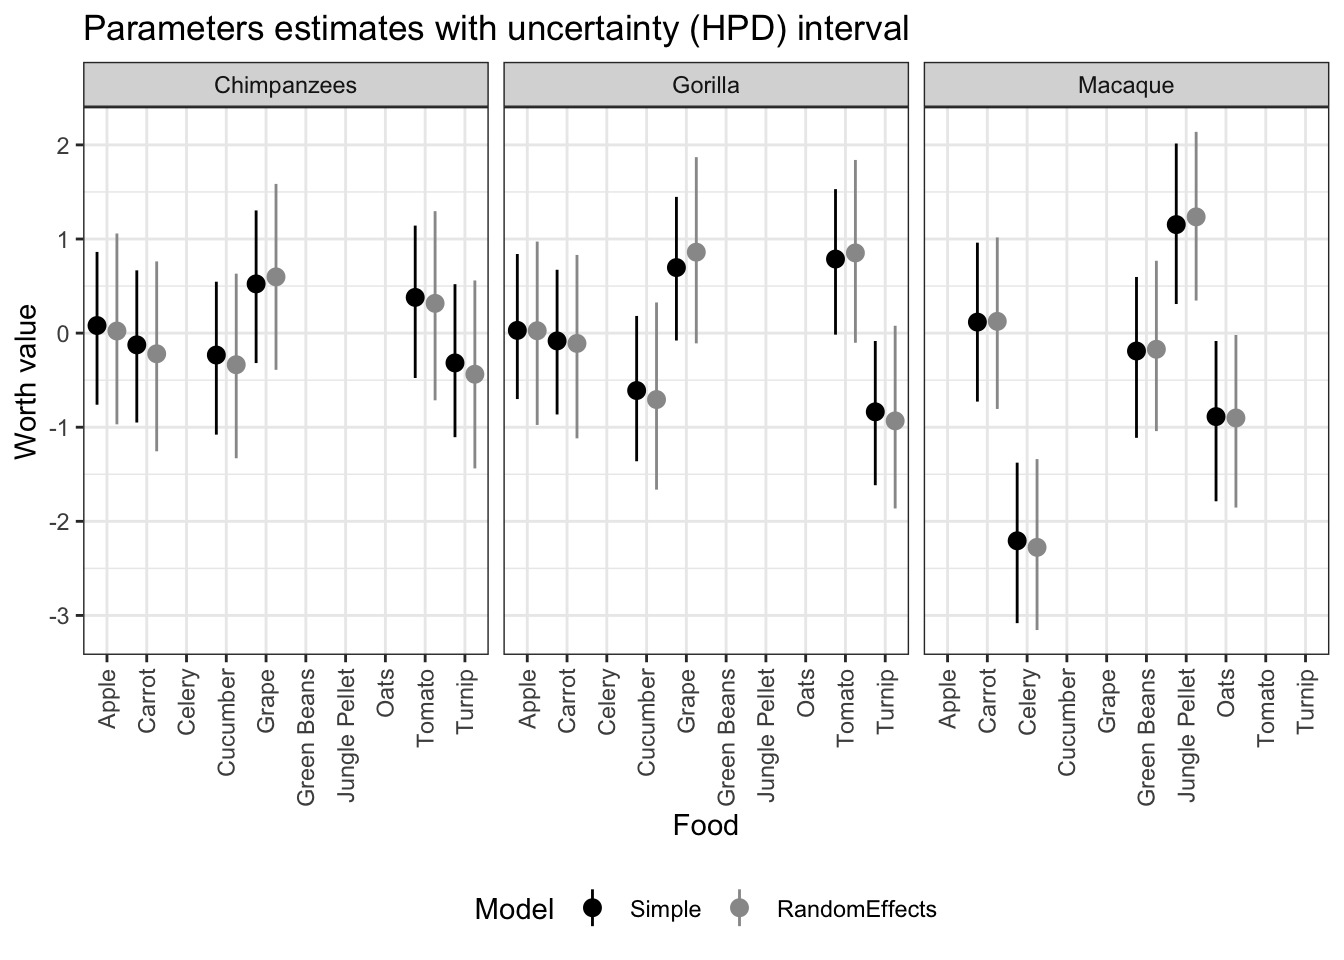
\includegraphics{bpcs-appendix_files/figure-latex/unnamed-chunk-69-1.pdf}

\hypertarget{probability-of-selecting-a-novel-stimuli}{%
\subsubsection{Probability of selecting a novel stimuli}\label{probability-of-selecting-a-novel-stimuli}}

We will create a the table of the predictions of selecting a novel stimuli (compared to the trained ones). This is replication of table II of the original paper (of course the results are not the same since we are using different models and estimation values)

For that, we first create a data frame of the new predictions for each species. Since our model uses random effects and we would need to specify each random effect to make the predictions we will do something slightly different. We will consider that the random effects will be zero, that is, which is equivalent to the average value of the random effects (remember that it has a mean of zero). One way to achieve this is by using the obtained coefficients in a submodel. This can be done in the bpcs package by using the model\_type option.

We ask for the data frame instead of the table because we will assemble the table manually.

\begin{Shaded}
\begin{Highlighting}[]
\CommentTok{# Create a data frame with all the pairs of food that we want to calculate}
\NormalTok{pairs_gor <-}
\StringTok{  }\KeywordTok{data.frame}\NormalTok{(}
    \DataTypeTok{image1 =} \KeywordTok{c}\NormalTok{(}
      \StringTok{'Apple'}\NormalTok{,}
      \StringTok{'Apple'}\NormalTok{,}
      \StringTok{'Apple'}\NormalTok{,}
      \StringTok{'Apple'}\NormalTok{,}
      \StringTok{'Tomato'}\NormalTok{,}
      \StringTok{'Tomato'}\NormalTok{,}
      \StringTok{'Tomato'}\NormalTok{,}
      \StringTok{'Tomato'}
\NormalTok{    ),}
    \DataTypeTok{image2 =} \KeywordTok{c}\NormalTok{(}
      \StringTok{'Cucumber'}\NormalTok{,}
      \StringTok{'Grape'}\NormalTok{,}
      \StringTok{'Turnip'}\NormalTok{,}
      \StringTok{'Carrot'}\NormalTok{,}
      \StringTok{'Cucumber'}\NormalTok{,}
      \StringTok{'Grape'}\NormalTok{,}
      \StringTok{'Turnip'}\NormalTok{,}
      \StringTok{'Carrot'}
\NormalTok{    )}
\NormalTok{  )}

\NormalTok{pairs_chip <-}
\StringTok{  }\KeywordTok{data.frame}\NormalTok{(}
    \DataTypeTok{image1 =} \KeywordTok{c}\NormalTok{(}
      \StringTok{'Apple'}\NormalTok{,}
      \StringTok{'Apple'}\NormalTok{,}
      \StringTok{'Apple'}\NormalTok{,}
      \StringTok{'Apple'}\NormalTok{,}
      \StringTok{'Tomato'}\NormalTok{,}
      \StringTok{'Tomato'}\NormalTok{,}
      \StringTok{'Tomato'}\NormalTok{,}
      \StringTok{'Tomato'}
\NormalTok{    ),}
    \DataTypeTok{image2 =} \KeywordTok{c}\NormalTok{(}
      \StringTok{'Cucumber'}\NormalTok{,}
      \StringTok{'Grape'}\NormalTok{,}
      \StringTok{'Turnip'}\NormalTok{,}
      \StringTok{'Carrot'}\NormalTok{,}
      \StringTok{'Cucumber'}\NormalTok{,}
      \StringTok{'Grape'}\NormalTok{,}
      \StringTok{'Turnip'}\NormalTok{,}
      \StringTok{'Carrot'}
\NormalTok{    )}
\NormalTok{  )}


\NormalTok{pairs_macaque <-}
\StringTok{  }\KeywordTok{data.frame}\NormalTok{(}
    \DataTypeTok{image1 =} \KeywordTok{c}\NormalTok{(}
      \StringTok{'Oats'}\NormalTok{,}
      \StringTok{'Oats'}\NormalTok{,}
      \StringTok{'Oats'}\NormalTok{,}
      \StringTok{'Oats'}\NormalTok{,}
      \StringTok{'Green Beans'}\NormalTok{,}
      \StringTok{'Green Beans'}\NormalTok{,}
      \StringTok{'Green Beans'}\NormalTok{,}
      \StringTok{'Green Beans'}
\NormalTok{    ),}
    \DataTypeTok{image2 =} \KeywordTok{c}\NormalTok{(}
      \StringTok{'Celery'}\NormalTok{,}
      \StringTok{'Jungle Pellet'}\NormalTok{,}
      \StringTok{'Peanuts'}\NormalTok{,}
      \StringTok{'Carrot'}\NormalTok{,}
      \StringTok{'Celery'}\NormalTok{,}
      \StringTok{'Jungle Pellet'}\NormalTok{,}
      \StringTok{'Peanuts'}\NormalTok{,}
      \StringTok{'Carrot'}
\NormalTok{    )}
\NormalTok{  )}


\NormalTok{prob_chip <-}
\StringTok{  }\KeywordTok{get_probabilities_df}\NormalTok{(}
\NormalTok{    m2_chip, }
    \DataTypeTok{newdata =}\NormalTok{ pairs_chip,}
    \DataTypeTok{model_type =} \StringTok{'bt'}\NormalTok{) }\CommentTok{#here we are assuming zero for the random effects}

\NormalTok{prob_macaque <-}
\StringTok{  }\KeywordTok{get_probabilities_df}\NormalTok{(}
\NormalTok{    m2_macaque, }
    \DataTypeTok{newdata =}\NormalTok{ pairs_macaque, }
    \DataTypeTok{model_type =} \StringTok{'bt'}\NormalTok{)}

\NormalTok{prob_gor <-}
\StringTok{  }\KeywordTok{get_probabilities_df}\NormalTok{(}
\NormalTok{    m2_gor, }
    \DataTypeTok{newdata =}\NormalTok{ pairs_gor, }
    \DataTypeTok{model_type =} \StringTok{'bt'}\NormalTok{)}

\CommentTok{#merging in a single df}
\NormalTok{prob_table <-}\StringTok{ }\KeywordTok{rbind}\NormalTok{(prob_gor, prob_chip, prob_macaque)}

\CommentTok{#since this is  a time consuming table to make let's also save it}
\KeywordTok{saveRDS}\NormalTok{(prob_table, }\StringTok{'prob_table.RDS'}\NormalTok{)}
\end{Highlighting}
\end{Shaded}

Now we can create the table

\begin{Shaded}
\begin{Highlighting}[]
\NormalTok{prob_table <-}\StringTok{ }\NormalTok{prob_table }\OperatorTok
\StringTok{  }\KeywordTok{mutate}\NormalTok{(}\DataTypeTok{Probability =}\NormalTok{ i_beats_j,}
         \DataTypeTok{OddsRatio =}\NormalTok{ Probability }\OperatorTok{/}\StringTok{ }\NormalTok{(}\DecValTok{1} \OperatorTok{-}\StringTok{ }\NormalTok{Probability))}

\NormalTok{prob_table }\OperatorTok
\StringTok{  }\NormalTok{dplyr}\OperatorTok{::}\KeywordTok{select}\NormalTok{(i, j, Probability, OddsRatio) }\OperatorTok
\StringTok{  }\KeywordTok{kable}\NormalTok{(}
    \DataTypeTok{caption =} \StringTok{'Posterior probabilities of the novel stimuli i being selected over the trained stimuli j'}\NormalTok{,}
    \DataTypeTok{booktabs =}\NormalTok{ T,}
    \DataTypeTok{digits =} \DecValTok{2}\NormalTok{,}
    \DataTypeTok{col.names =} \KeywordTok{c}\NormalTok{(}\StringTok{'Item i'}\NormalTok{, }\StringTok{'Item j'}\NormalTok{, }\StringTok{'Probability'}\NormalTok{, }\StringTok{'Odds Ratio'}\NormalTok{)}
\NormalTok{  ) }\OperatorTok
\StringTok{  }\NormalTok{kableExtra}\OperatorTok{::}\KeywordTok{kable_styling}\NormalTok{(}\DataTypeTok{bootstrap_options =} \KeywordTok{c}\NormalTok{(}\StringTok{"striped"}\NormalTok{, }\StringTok{"hover"}\NormalTok{, }\StringTok{"condensed"}\NormalTok{, }\StringTok{"responsive"}\NormalTok{)) }\OperatorTok
\StringTok{  }\NormalTok{kableExtra}\OperatorTok{::}\KeywordTok{pack_rows}\NormalTok{(}\StringTok{"Gorilla"}\NormalTok{, }\DecValTok{1}\NormalTok{, }\DecValTok{8}\NormalTok{) }\OperatorTok
\StringTok{  }\NormalTok{kableExtra}\OperatorTok{::}\KeywordTok{pack_rows}\NormalTok{(}\StringTok{"Chimpanzee"}\NormalTok{, }\DecValTok{9}\NormalTok{, }\DecValTok{16}\NormalTok{) }\OperatorTok
\StringTok{  }\NormalTok{kableExtra}\OperatorTok{::}\KeywordTok{pack_rows}\NormalTok{(}\StringTok{"Macaque"}\NormalTok{, }\DecValTok{17}\NormalTok{, }\DecValTok{24}\NormalTok{) }\OperatorTok\StringTok{ }
\StringTok{  }\NormalTok{kableExtra}\OperatorTok{::}\KeywordTok{scroll_box}\NormalTok{(}\DataTypeTok{width =} \StringTok{"100%"}\NormalTok{)}
\end{Highlighting}
\end{Shaded}

\begin{table}

\caption{\label{tab:unnamed-chunk-72}Posterior probabilities of the novel stimuli i being selected over the trained stimuli j}
\centering
\begin{tabular}[t]{llrr}
\toprule
Item i & Item j & Probability & Odds Ratio\\
\midrule
\addlinespace[0.3em]
\multicolumn{4}{l}{\textbf{Gorilla}}\\
\hspace{1em}Apple & Cucumber & 0.78 & 3.55\\
\hspace{1em}Apple & Grape & 0.35 & 0.54\\
\hspace{1em}Apple & Turnip & 0.75 & 3.00\\
\hspace{1em}Apple & Carrot & 0.57 & 1.33\\
\hspace{1em}Tomato & Cucumber & 0.80 & 4.00\\
\hspace{1em}Tomato & Grape & 0.48 & 0.92\\
\hspace{1em}Tomato & Turnip & 0.79 & 3.76\\
\hspace{1em}Tomato & Carrot & 0.69 & 2.23\\
\addlinespace[0.3em]
\multicolumn{4}{l}{\textbf{Chimpanzee}}\\
\hspace{1em}Apple & Cucumber & 0.64 & 1.78\\
\hspace{1em}Apple & Grape & 0.42 & 0.72\\
\hspace{1em}Apple & Turnip & 0.55 & 1.22\\
\hspace{1em}Apple & Carrot & 0.51 & 1.04\\
\hspace{1em}Tomato & Cucumber & 0.54 & 1.17\\
\hspace{1em}Tomato & Grape & 0.37 & 0.59\\
\hspace{1em}Tomato & Turnip & 0.69 & 2.23\\
\hspace{1em}Tomato & Carrot & 0.64 & 1.78\\
\addlinespace[0.3em]
\multicolumn{4}{l}{\textbf{Macaque}}\\
\hspace{1em}Oats & Celery & 0.76 & 3.17\\
\hspace{1em}Oats & Jungle Pellet & 0.11 & 0.12\\
\hspace{1em}Oats & Peanuts & 0.06 & 0.06\\
\hspace{1em}Oats & Carrot & 0.23 & 0.30\\
\hspace{1em}Green Beans & Celery & 0.88 & 7.33\\
\hspace{1em}Green Beans & Jungle Pellet & 0.26 & 0.35\\
\hspace{1em}Green Beans & Peanuts & 0.10 & 0.11\\
\hspace{1em}Green Beans & Carrot & 0.45 & 0.82\\
\bottomrule
\end{tabular}
\end{table}

\hypertarget{studyIII}{%
\chapter{Re-analysis 3}\label{studyIII}}

This re-analysis is from the study

\begin{quote}
Marton, Giulia, et al.~``Patients' health locus of control and preferences about the role that they want to play in the medical decision-making process.'' Psychology, Health \& Medicine (2020): 1-7
\end{quote}

\begin{Shaded}
\begin{Highlighting}[]
\KeywordTok{library}\NormalTok{(bpcs)}
\KeywordTok{library}\NormalTok{(tidyverse)}
\KeywordTok{library}\NormalTok{(knitr)}
\KeywordTok{library}\NormalTok{(loo)}
\KeywordTok{options}\NormalTok{(}\DataTypeTok{mc.cores =}\NormalTok{ parallel}\OperatorTok{::}\KeywordTok{detectCores}\NormalTok{())}
\NormalTok{rstan}\OperatorTok{::}\KeywordTok{rstan_options}\NormalTok{(}\DataTypeTok{auto_write =} \OtherTok{TRUE}\NormalTok{)}
\KeywordTok{set.seed}\NormalTok{(}\DecValTok{99}\NormalTok{)}
\end{Highlighting}
\end{Shaded}

\hypertarget{importing-the-data-2}{%
\section{Importing the data}\label{importing-the-data-2}}

The data from this paper was made available upon request and below we exemplify a few rows of how the original dataset looks like.
Let's starting importing the data.

\begin{Shaded}
\begin{Highlighting}[]
\NormalTok{d<-}\KeywordTok{read.table}\NormalTok{(}\StringTok{"data/MHLC.txt"}\NormalTok{, }\DataTypeTok{sep=}\StringTok{"}\CharTok{\textbackslash{}t}\StringTok{"}\NormalTok{, }\DataTypeTok{header=}\NormalTok{T)}
\NormalTok{d<-}\KeywordTok{as.data.frame}\NormalTok{(d)}
\KeywordTok{sample_n}\NormalTok{(d, }\DataTypeTok{size=}\DecValTok{5}\NormalTok{) }\OperatorTok\StringTok{ }
\StringTok{  }\KeywordTok{kable}\NormalTok{(}\DataTypeTok{caption =} \StringTok{'Sample of rows from the original data'}\NormalTok{) }\OperatorTok\StringTok{ }
\StringTok{  }\NormalTok{kableExtra}\OperatorTok{::}\KeywordTok{kable_styling}\NormalTok{(}\DataTypeTok{bootstrap_options =} \KeywordTok{c}\NormalTok{(}\StringTok{"striped"}\NormalTok{, }\StringTok{"hover"}\NormalTok{, }\StringTok{"condensed"}\NormalTok{, }\StringTok{"responsive"}\NormalTok{)) }\OperatorTok\StringTok{ }
\StringTok{  }\NormalTok{kableExtra}\OperatorTok{::}\KeywordTok{scroll_box}\NormalTok{(}\DataTypeTok{width =} \StringTok{"100%"}\NormalTok{)}
\end{Highlighting}
\end{Shaded}

\begin{table}

\caption{\label{tab:unnamed-chunk-75}Sample of rows from the original data}
\centering
\begin{tabular}[t]{r|r|r|r|r|r|r|r|r|r|r|r|r|r|r|r}
\hline
AB & AC & BC & AD & BD & CD & AE & BE & CE & DE & GENDER & MHLC\_INTERNAL & MHLC\_CHANCE & MHLC\_DOCTORS & MHLC\_OTHER\_PEOPLE & Age\\
\hline
1 & 1 & 1 & 1 & 1 & 1 & 1 & 1 & 1 & 1 & 2 & 16 & 14 & 12 & 10 & 56\\
\hline
1 & 1 & 1 & 1 & 1 & 0 & 0 & 0 & 0 & 0 & 2 & 23 & 13 & 14 & 7 & 53\\
\hline
1 & 1 & 1 & 0 & 0 & 0 & 0 & 0 & 0 & 0 & 1 & 19 & 6 & 9 & 5 & 58\\
\hline
1 & 1 & 1 & 1 & 1 & 0 & 1 & 0 & 0 & 0 & 2 & 19 & 7 & 7 & 8 & 27\\
\hline
1 & 1 & 1 & 1 & 0 & 0 & 0 & 0 & 0 & 0 & 1 & 14 & 12 & 11 & 5 & 28\\
\hline
\end{tabular}
\end{table}

As we can see, the data is in a wide format. Before we pivot it to longer let's add a column that indicates the subject ID.

\begin{Shaded}
\begin{Highlighting}[]
\NormalTok{d <-}\StringTok{ }\NormalTok{d }\OperatorTok\StringTok{ }\KeywordTok{mutate}\NormalTok{(}\DataTypeTok{SubjectID =} \KeywordTok{row_number}\NormalTok{())}
\end{Highlighting}
\end{Shaded}

Now let's pivot it to the longer format

\begin{Shaded}
\begin{Highlighting}[]
\NormalTok{cols_to_pivot<-}\KeywordTok{colnames}\NormalTok{(d)[}\DecValTok{1}\OperatorTok{:}\DecValTok{10}\NormalTok{]}
\NormalTok{d_longer<-tidyr}\OperatorTok{::}\KeywordTok{pivot_longer}\NormalTok{(d, }\DataTypeTok{cols=}\KeywordTok{all_of}\NormalTok{(cols_to_pivot), }\DataTypeTok{names_to=}\StringTok{'comparison'}\NormalTok{, }\DataTypeTok{values_to=}\StringTok{'y'}\NormalTok{)}
\end{Highlighting}
\end{Shaded}

Now let's divide the comparison into two vectors (choice0 and choice1). So it fits the bpcs format

\begin{Shaded}
\begin{Highlighting}[]
\NormalTok{comp_cols <-}\StringTok{ }\KeywordTok{str_split_fixed}\NormalTok{(d_longer}\OperatorTok{$}\NormalTok{comparison, }\StringTok{""}\NormalTok{, }\DecValTok{2}\NormalTok{)}
\NormalTok{d_longer}\OperatorTok{$}\NormalTok{choice0 <-}\StringTok{ }\NormalTok{comp_cols[,}\DecValTok{1}\NormalTok{]}
\NormalTok{d_longer}\OperatorTok{$}\NormalTok{choice1 <-}\StringTok{ }\NormalTok{comp_cols[,}\DecValTok{2}\NormalTok{]}
\end{Highlighting}
\end{Shaded}

The data frame now looks like this:

\begin{Shaded}
\begin{Highlighting}[]
\NormalTok{dplyr}\OperatorTok{::}\KeywordTok{sample_n}\NormalTok{(d_longer, }\DataTypeTok{size=}\DecValTok{10}\NormalTok{) }\OperatorTok\StringTok{ }
\StringTok{  }\KeywordTok{kable}\NormalTok{() }\OperatorTok\StringTok{ }
\StringTok{  }\NormalTok{kableExtra}\OperatorTok{::}\KeywordTok{kable_styling}\NormalTok{(}\DataTypeTok{bootstrap_options =} \KeywordTok{c}\NormalTok{(}\StringTok{"striped"}\NormalTok{, }\StringTok{"hover"}\NormalTok{, }\StringTok{"condensed"}\NormalTok{, }\StringTok{"responsive"}\NormalTok{)) }\OperatorTok\StringTok{ }
\StringTok{  }\NormalTok{kableExtra}\OperatorTok{::}\KeywordTok{scroll_box}\NormalTok{(}\DataTypeTok{width =} \StringTok{"100%"}\NormalTok{)}
\end{Highlighting}
\end{Shaded}

\begin{table}[H]
\centering
\begin{tabular}{r|r|r|r|r|r|r|l|r|l|l}
\hline
GENDER & MHLC\_INTERNAL & MHLC\_CHANCE & MHLC\_DOCTORS & MHLC\_OTHER\_PEOPLE & Age & SubjectID & comparison & y & choice0 & choice1\\
\hline
1 & 22 & 6 & 15 & 14 & 31 & 96 & BE & 1 & B & E\\
\hline
2 & 20 & 17 & 8 & 9 & 26 & 125 & DE & 0 & D & E\\
\hline
2 & 30 & 30 & 15 & 15 & 27 & 116 & AC & 1 & A & C\\
\hline
2 & 23 & 8 & 14 & 9 & 55 & 36 & BE & 1 & B & E\\
\hline
2 & 23 & 18 & 13 & 11 & 53 & 42 & CD & 0 & C & D\\
\hline
1 & 20 & 17 & 14 & 9 & 37 & 79 & AB & 1 & A & B\\
\hline
2 & 21 & 23 & 13 & 11 & 78 & 2 & DE & 0 & D & E\\
\hline
2 & 20 & 23 & 8 & 13 & 30 & 100 & CD & 1 & C & D\\
\hline
2 & 19 & 19 & 17 & 9 & 34 & 93 & AE & 1 & A & E\\
\hline
2 & 33 & 31 & 8 & 13 & 45 & 58 & DE & 1 & D & E\\
\hline
\end{tabular}
\end{table}

Now that we have setup the data frame correctly for the bpcs package, we can use it to model the problem.

Let's just rename a few values so it is easier to understand.

\begin{Shaded}
\begin{Highlighting}[]
\CommentTok{#choice0}
\NormalTok{d_longer}\OperatorTok{$}\NormalTok{choice0 <-}\StringTok{ }\KeywordTok{recode}\NormalTok{(d_longer}\OperatorTok{$}\NormalTok{choice0, }\StringTok{'A'}\NormalTok{=}\StringTok{'Active'}\NormalTok{) }
\NormalTok{d_longer}\OperatorTok{$}\NormalTok{choice0 <-}\StringTok{ }\KeywordTok{recode}\NormalTok{(d_longer}\OperatorTok{$}\NormalTok{choice0, }\StringTok{'B'}\NormalTok{=}\StringTok{'Active-Collaborative'}\NormalTok{) }
\NormalTok{d_longer}\OperatorTok{$}\NormalTok{choice0 <-}\StringTok{ }\KeywordTok{recode}\NormalTok{(d_longer}\OperatorTok{$}\NormalTok{choice0, }\StringTok{'C'}\NormalTok{=}\StringTok{'Collaborative'}\NormalTok{) }
\NormalTok{d_longer}\OperatorTok{$}\NormalTok{choice0 <-}\StringTok{ }\KeywordTok{recode}\NormalTok{(d_longer}\OperatorTok{$}\NormalTok{choice0, }\StringTok{'D'}\NormalTok{=}\StringTok{'Passive-Collaborative'}\NormalTok{) }
\NormalTok{d_longer}\OperatorTok{$}\NormalTok{choice0 <-}\StringTok{ }\KeywordTok{recode}\NormalTok{(d_longer}\OperatorTok{$}\NormalTok{choice0, }\StringTok{'E'}\NormalTok{=}\StringTok{'Passive'}\NormalTok{) }
\CommentTok{#choice1}
\NormalTok{d_longer}\OperatorTok{$}\NormalTok{choice1 <-}\StringTok{ }\KeywordTok{recode}\NormalTok{(d_longer}\OperatorTok{$}\NormalTok{choice1, }\StringTok{'A'}\NormalTok{=}\StringTok{'Active'}\NormalTok{) }
\NormalTok{d_longer}\OperatorTok{$}\NormalTok{choice1 <-}\StringTok{ }\KeywordTok{recode}\NormalTok{(d_longer}\OperatorTok{$}\NormalTok{choice1, }\StringTok{'B'}\NormalTok{=}\StringTok{'Active-Collaborative'}\NormalTok{) }
\NormalTok{d_longer}\OperatorTok{$}\NormalTok{choice1 <-}\StringTok{ }\KeywordTok{recode}\NormalTok{(d_longer}\OperatorTok{$}\NormalTok{choice1, }\StringTok{'C'}\NormalTok{=}\StringTok{'Collaborative'}\NormalTok{) }
\NormalTok{d_longer}\OperatorTok{$}\NormalTok{choice1 <-}\StringTok{ }\KeywordTok{recode}\NormalTok{(d_longer}\OperatorTok{$}\NormalTok{choice1, }\StringTok{'D'}\NormalTok{=}\StringTok{'Passive-Collaborative'}\NormalTok{) }
\NormalTok{d_longer}\OperatorTok{$}\NormalTok{choice1 <-}\StringTok{ }\KeywordTok{recode}\NormalTok{(d_longer}\OperatorTok{$}\NormalTok{choice1, }\StringTok{'E'}\NormalTok{=}\StringTok{'Passive'}\NormalTok{)}
\end{Highlighting}
\end{Shaded}

Our final step in the preparation of the dataset is to standardize the values of the MHLOC scales. The values provided in the dataset correspond to the sum of the values of the scale and ranges from 3-18 or from 6-36. Therefore we will scale them accordingly for more stable inference

\begin{Shaded}
\begin{Highlighting}[]
\NormalTok{d_longer <-}\StringTok{ }\NormalTok{d_longer }\OperatorTok\StringTok{ }
\StringTok{  }\KeywordTok{mutate}\NormalTok{(}\DataTypeTok{Internal =} \KeywordTok{scale}\NormalTok{(MHLC_INTERNAL),}
         \DataTypeTok{Chance =} \KeywordTok{scale}\NormalTok{(MHLC_CHANCE),}
         \DataTypeTok{Doctors =} \KeywordTok{scale}\NormalTok{(MHLC_DOCTORS),}
         \DataTypeTok{OtherPeople =} \KeywordTok{scale}\NormalTok{(MHLC_OTHER_PEOPLE))}
\end{Highlighting}
\end{Shaded}

The final modified dataset looks like:

\begin{Shaded}
\begin{Highlighting}[]
\KeywordTok{sample_n}\NormalTok{(d_longer, }\DataTypeTok{size=}\DecValTok{10}\NormalTok{) }\OperatorTok\StringTok{ }
\StringTok{  }\KeywordTok{kable}\NormalTok{() }\OperatorTok\StringTok{ }
\StringTok{  }\NormalTok{kableExtra}\OperatorTok{::}\KeywordTok{kable_styling}\NormalTok{(}\DataTypeTok{bootstrap_options =} \KeywordTok{c}\NormalTok{(}\StringTok{"striped"}\NormalTok{, }\StringTok{"hover"}\NormalTok{, }\StringTok{"condensed"}\NormalTok{, }\StringTok{"responsive"}\NormalTok{)) }\OperatorTok\StringTok{ }
\StringTok{  }\NormalTok{kableExtra}\OperatorTok{::}\KeywordTok{scroll_box}\NormalTok{(}\DataTypeTok{width =} \StringTok{"100%"}\NormalTok{)}
\end{Highlighting}
\end{Shaded}

\begin{table}[H]
\centering
\begin{tabular}{r|r|r|r|r|r|r|l|r|l|l|r|r|r|r}
\hline
GENDER & MHLC\_INTERNAL & MHLC\_CHANCE & MHLC\_DOCTORS & MHLC\_OTHER\_PEOPLE & Age & SubjectID & comparison & y & choice0 & choice1 & Internal & Chance & Doctors & OtherPeople\\
\hline
2 & 18 & 11 & 9 & 7 & 57 & 27 & BD & 1 & Active-Collaborative & Passive-Collaborative & -0.4347094 & -0.61218263 & -0.76052743 & -0.4611581\\
\hline
1 & 18 & 31 & 15 & 8 & 44 & 60 & DE & 0 & Passive-Collaborative & Passive & -0.4347094 & 2.96961250 & 1.23422737 & -0.1135857\\
\hline
2 & 15 & 17 & 15 & 9 & 27 & 119 & AC & 1 & Active & Collaborative & -1.0563033 & 0.46235591 & 1.23422737 & 0.2339866\\
\hline
1 & 18 & 31 & 15 & 8 & 44 & 60 & BE & 0 & Active-Collaborative & Passive & -0.4347094 & 2.96961250 & 1.23422737 & -0.1135857\\
\hline
2 & 23 & 18 & 13 & 11 & 53 & 42 & CD & 0 & Collaborative & Passive-Collaborative & 0.6012804 & 0.64144566 & 0.56930911 & 0.9291313\\
\hline
1 & 21 & 13 & 11 & 7 & 53 & 40 & BE & 0 & Active-Collaborative & Passive & 0.1868844 & -0.25400312 & -0.09560916 & -0.4611581\\
\hline
2 & 25 & 14 & 14 & 10 & 61 & 14 & AC & 1 & Active & Collaborative & 1.0156763 & -0.07491336 & 0.90176824 & 0.5815589\\
\hline
2 & 30 & 14 & 10 & 9 & 63 & 8 & BE & 0 & Active-Collaborative & Passive & 2.0516661 & -0.07491336 & -0.42806830 & 0.2339866\\
\hline
2 & 15 & 15 & 12 & 8 & 36 & 87 & BD & 1 & Active-Collaborative & Passive-Collaborative & -1.0563033 & 0.10417639 & 0.23684997 & -0.1135857\\
\hline
1 & 15 & 14 & 9 & 6 & NA & 1 & AE & 0 & Active & Passive & -1.0563033 & -0.07491336 & -0.76052743 & -0.8087304\\
\hline
\end{tabular}
\end{table}

Now we can proceed with the analysis.

\hypertarget{simple-bradley-terry-models}{%
\section{Simple Bradley-Terry models}\label{simple-bradley-terry-models}}

Let's start with a simple BT without considering any subject predictors. Just to evaluate the average probability of people being Active, Active-Collaborative, Collaborative, Passive-Collaborative or Passive.

\begin{Shaded}
\begin{Highlighting}[]
\NormalTok{m1 <-}
\StringTok{  }\KeywordTok{bpc}\NormalTok{(}
\NormalTok{    d_longer,}
    \DataTypeTok{player0 =} \StringTok{'choice0'}\NormalTok{,}
    \DataTypeTok{player1 =} \StringTok{'choice1'}\NormalTok{,}
    \DataTypeTok{result_column =} \StringTok{'y'}\NormalTok{,}
    \DataTypeTok{model_type =} \StringTok{'bt'}\NormalTok{,}
    \DataTypeTok{priors =} \KeywordTok{list}\NormalTok{(}\DataTypeTok{prior_lambda_std =} \FloatTok{1.0}\NormalTok{),}
    \DataTypeTok{iter =} \DecValTok{3000}
\NormalTok{  )}
\KeywordTok{save_bpc_model}\NormalTok{(m1, }\StringTok{'m_hloc'}\NormalTok{, }\StringTok{'fittedmodels'}\NormalTok{)}
\end{Highlighting}
\end{Shaded}

Let's investigate model convergence with shinystan. Everything seems fine.

\begin{Shaded}
\begin{Highlighting}[]
\KeywordTok{launch_shinystan}\NormalTok{(m1)}
\end{Highlighting}
\end{Shaded}

Now let's get the waic

\begin{Shaded}
\begin{Highlighting}[]
\NormalTok{m1_waic <-}\StringTok{ }\KeywordTok{get_waic}\NormalTok{(m1)}
\NormalTok{m1_waic}
\end{Highlighting}
\end{Shaded}

\begin{verbatim}
## 
## Computed from 8000 by 1530 log-likelihood matrix
## 
##           Estimate   SE
## elpd_waic   -711.2 21.9
## p_waic         3.9  0.2
## waic        1422.4 43.9
\end{verbatim}

\hypertarget{subject-predictors-model}{%
\section{Subject predictors model}\label{subject-predictors-model}}

We have different HLC that can be used as predictors for the response. Let's create a single model with all the predictors.

\begin{Shaded}
\begin{Highlighting}[]
\NormalTok{m2 <-}
\StringTok{  }\KeywordTok{bpc}\NormalTok{(}
\NormalTok{    d_longer,}
    \DataTypeTok{player0 =} \StringTok{'choice0'}\NormalTok{,}
    \DataTypeTok{player1 =} \StringTok{'choice1'}\NormalTok{,}
    \DataTypeTok{result_column =} \StringTok{'y'}\NormalTok{,}
    \DataTypeTok{subject_predictors =} \KeywordTok{c}\NormalTok{(}\StringTok{'Internal'}\NormalTok{, }\StringTok{'Chance'}\NormalTok{, }\StringTok{'Doctors'}\NormalTok{, }\StringTok{'OtherPeople'}\NormalTok{),}
    \DataTypeTok{model_type =} \StringTok{'bt-subjectpredictors'}\NormalTok{,}
    \DataTypeTok{priors =} \KeywordTok{list}\NormalTok{(}\DataTypeTok{prior_lambda_std =} \FloatTok{1.0}\NormalTok{,}
                  \DataTypeTok{prior_S_std =} \FloatTok{1.0}\NormalTok{),}
    \DataTypeTok{iter =} \DecValTok{3000}
\NormalTok{  )}
\KeywordTok{save_bpc_model}\NormalTok{(m2, }\StringTok{'m_mhloc_subjectpred'}\NormalTok{, }\StringTok{'fittedmodels'}\NormalTok{)}
\end{Highlighting}
\end{Shaded}

Diagnostics

\begin{Shaded}
\begin{Highlighting}[]
\KeywordTok{launch_shinystan}\NormalTok{(m2)}
\end{Highlighting}
\end{Shaded}

\begin{Shaded}
\begin{Highlighting}[]
\NormalTok{m2_waic <-}\StringTok{ }\KeywordTok{get_waic}\NormalTok{(m2)}
\end{Highlighting}
\end{Shaded}

\hypertarget{subject-predictors-and-random-effects}{%
\section{Subject predictors and random effects}\label{subject-predictors-and-random-effects}}

Now let's create a third model that also compensate for multiple judgment with a random effects variable.

This model adds 153*4 variables, so sampling will take longer and be a bit more complex.

\begin{Shaded}
\begin{Highlighting}[]
\NormalTok{m3 <-}
\StringTok{  }\KeywordTok{bpc}\NormalTok{(}
\NormalTok{    d_longer,}
    \DataTypeTok{player0 =} \StringTok{'choice0'}\NormalTok{,}
    \DataTypeTok{player1 =} \StringTok{'choice1'}\NormalTok{,}
    \DataTypeTok{result_column =} \StringTok{'y'}\NormalTok{,}
    \DataTypeTok{subject_predictors =} \KeywordTok{c}\NormalTok{(}\StringTok{'Internal'}\NormalTok{, }\StringTok{'Chance'}\NormalTok{, }\StringTok{'Doctors'}\NormalTok{, }\StringTok{'OtherPeople'}\NormalTok{),}
    \DataTypeTok{cluster =} \KeywordTok{c}\NormalTok{(}\StringTok{'SubjectID'}\NormalTok{),}
    \DataTypeTok{model_type =} \StringTok{'bt-subjectpredictors-U'}\NormalTok{,}
    \DataTypeTok{priors =} \KeywordTok{list}\NormalTok{(}\DataTypeTok{prior_lambda_std =} \FloatTok{1.0}\NormalTok{,}
                  \DataTypeTok{prior_S_std =} \FloatTok{1.0}\NormalTok{,}
                  \DataTypeTok{prior_U1_std =} \FloatTok{1.0}\NormalTok{),}
    \DataTypeTok{iter =} \DecValTok{3000}
\NormalTok{  )}
\KeywordTok{save_bpc_model}\NormalTok{(m3, }\StringTok{'m_mhloc_subjectpred_U'}\NormalTok{, }\StringTok{'fittedmodels'}\NormalTok{)}
\end{Highlighting}
\end{Shaded}

Diagnostics

\begin{Shaded}
\begin{Highlighting}[]
\KeywordTok{launch_shinystan}\NormalTok{(m3)}
\end{Highlighting}
\end{Shaded}

\begin{Shaded}
\begin{Highlighting}[]
\NormalTok{m3_waic <-}\StringTok{ }\KeywordTok{get_waic}\NormalTok{(m3)}
\end{Highlighting}
\end{Shaded}

\hypertarget{comparing-the-waic}{%
\section{Comparing the WAIC}\label{comparing-the-waic}}

Let's compare the WAIC of the three models

\begin{Shaded}
\begin{Highlighting}[]
\NormalTok{loo}\OperatorTok{::}\KeywordTok{loo_compare}\NormalTok{(m1_waic,m2_waic, m3_waic)}
\end{Highlighting}
\end{Shaded}

\begin{verbatim}
##        elpd_diff se_diff
## model3    0.0       0.0 
## model2 -226.7      14.8 
## model1 -248.8      16.1
\end{verbatim}

\hypertarget{plots-and-tables}{%
\section{Plots and tables}\label{plots-and-tables}}

Now that we see that all models have proper convergence and that the model m3 has a better fit we will generate some plots and tables to help understand the problem

\begin{Shaded}
\begin{Highlighting}[]
\NormalTok{lambda <-}\StringTok{ }\KeywordTok{get_parameters}\NormalTok{(m3, }\DataTypeTok{params =} \StringTok{'lambda'}\NormalTok{, }\DataTypeTok{n_eff =}\NormalTok{ F)}
\NormalTok{Spar <-}\StringTok{ }\KeywordTok{get_parameters}\NormalTok{(m3, }\DataTypeTok{params =} \StringTok{'S'}\NormalTok{, }\DataTypeTok{n_eff =}\NormalTok{ F)}
\NormalTok{U_std <-}\StringTok{ }\KeywordTok{get_parameters}\NormalTok{(m3, }\DataTypeTok{params =} \StringTok{'U1_std'}\NormalTok{, }\DataTypeTok{n_eff =}\NormalTok{ F)}
\end{Highlighting}
\end{Shaded}

Let's create a custom table based on these parameters. But first we will rename the parameters a bit so the table reads a bit better. We are here removing the S and the lambda from the parameter

\begin{Shaded}
\begin{Highlighting}[]
\NormalTok{lambda}\OperatorTok{$}\NormalTok{Parameter <-}\StringTok{  }\NormalTok{stringr}\OperatorTok{::}\KeywordTok{str_sub}\NormalTok{(lambda}\OperatorTok{$}\NormalTok{Parameter,}\DataTypeTok{start =} \DecValTok{8}\NormalTok{, }\DataTypeTok{end=}\OperatorTok{-}\DecValTok{2}\NormalTok{)}
\NormalTok{Spar}\OperatorTok{$}\NormalTok{Parameter <-}\StringTok{ }\NormalTok{stringr}\OperatorTok{::}\KeywordTok{str_sub}\NormalTok{(Spar}\OperatorTok{$}\NormalTok{Parameter,}\DataTypeTok{start =} \DecValTok{3}\NormalTok{, }\DataTypeTok{end=}\OperatorTok{-}\DecValTok{2}\NormalTok{)}
\end{Highlighting}
\end{Shaded}

\hypertarget{table-lambda-and-u}{%
\subsection{Table lambda and U}\label{table-lambda-and-u}}

Now we can create the table

\begin{Shaded}
\begin{Highlighting}[]
\CommentTok{#merge the datasets}
\NormalTok{df_table <-}\StringTok{ }\KeywordTok{rbind}\NormalTok{(lambda, U_std) }
\CommentTok{#creating the table}
\NormalTok{df_table }\OperatorTok\StringTok{ }
\StringTok{  }\KeywordTok{kable}\NormalTok{(}\DataTypeTok{caption =} \StringTok{'Lambda parameters of the model and the random effects standard deviation'}\NormalTok{, }
        \DataTypeTok{digits =} \DecValTok{2}\NormalTok{,}
        \DataTypeTok{col.names =} \KeywordTok{c}\NormalTok{(}\StringTok{'Parameter'}\NormalTok{, }\StringTok{'Mean'}\NormalTok{,}\StringTok{'HPD lower'}\NormalTok{, }\StringTok{'HPD lower'}\NormalTok{)) }\OperatorTok\StringTok{ }
\StringTok{  }\NormalTok{kableExtra}\OperatorTok{::}\KeywordTok{kable_styling}\NormalTok{(}\DataTypeTok{bootstrap_options =} \KeywordTok{c}\NormalTok{(}\StringTok{"striped"}\NormalTok{, }\StringTok{"hover"}\NormalTok{, }\StringTok{"condensed"}\NormalTok{, }\StringTok{"responsive"}\NormalTok{)) }\OperatorTok\StringTok{ }
\StringTok{  }\NormalTok{kableExtra}\OperatorTok{::}\KeywordTok{scroll_box}\NormalTok{(}\DataTypeTok{width =} \StringTok{"100%"}\NormalTok{)}
\end{Highlighting}
\end{Shaded}

\begin{table}

\caption{\label{tab:unnamed-chunk-98}Lambda parameters of the model and the random effects standard deviation}
\centering
\begin{tabular}[t]{l|r|r|r}
\hline
Parameter & Mean & HPD lower & HPD lower\\
\hline
Active & -2.11 & -3.04 & -1.08\\
\hline
Active-Collaborative & 1.40 & 0.44 & 2.38\\
\hline
Collaborative & 3.21 & 2.08 & 4.21\\
\hline
Passive-Collaborative & 0.85 & -0.07 & 1.84\\
\hline
Passive & -3.32 & -4.43 & -2.34\\
\hline
U1\_std & 2.32 & 1.89 & 2.78\\
\hline
\end{tabular}
\end{table}

\hypertarget{subject-predictors-table}{%
\subsection{Subject predictors table}\label{subject-predictors-table}}

\begin{Shaded}
\begin{Highlighting}[]
\NormalTok{S <-}\StringTok{ }\NormalTok{Spar }\OperatorTok\StringTok{ }\NormalTok{tidyr}\OperatorTok{::}\KeywordTok{separate}\NormalTok{(Parameter,}\KeywordTok{c}\NormalTok{(}\StringTok{'Role'}\NormalTok{,}\StringTok{'MHLOC'}\NormalTok{), }\DataTypeTok{sep=}\StringTok{","}\NormalTok{)}
\NormalTok{S}\OperatorTok{$}\NormalTok{MHLOC <-}\StringTok{ }\KeywordTok{recode}\NormalTok{(S}\OperatorTok{$}\NormalTok{MHLOC, }\StringTok{'OtherPeople'}\NormalTok{=}\StringTok{ 'Other people'}\NormalTok{)}
\end{Highlighting}
\end{Shaded}

\begin{Shaded}
\begin{Highlighting}[]
\NormalTok{S }\OperatorTok\StringTok{ }
\StringTok{  }\NormalTok{dplyr}\OperatorTok{::}\KeywordTok{arrange}\NormalTok{(Role) }\OperatorTok\StringTok{ }
\StringTok{  }\KeywordTok{select}\NormalTok{(}\OperatorTok{-}\NormalTok{Role) }\OperatorTok\StringTok{ }
\StringTok{  }\KeywordTok{kable}\NormalTok{(}\DataTypeTok{format=}\StringTok{'html'}\NormalTok{,}
        \DataTypeTok{caption =} \StringTok{'Subject predictors parameters by role'}\NormalTok{, }
        \DataTypeTok{digits =} \DecValTok{2}\NormalTok{,}
        \DataTypeTok{col.names =} \KeywordTok{c}\NormalTok{(}\StringTok{'Parameter'}\NormalTok{, }\StringTok{'Mean'}\NormalTok{,}\StringTok{'HPD lower'}\NormalTok{, }\StringTok{'HPD lower'}\NormalTok{),}
        \DataTypeTok{booktabs=}\NormalTok{T) }\OperatorTok\StringTok{ }
\StringTok{  }\NormalTok{kableExtra}\OperatorTok{::}\KeywordTok{kable_styling}\NormalTok{(}\DataTypeTok{bootstrap_options =} \KeywordTok{c}\NormalTok{(}\StringTok{"striped"}\NormalTok{, }\StringTok{"hover"}\NormalTok{, }\StringTok{"condensed"}\NormalTok{, }\StringTok{"responsive"}\NormalTok{)) }\OperatorTok\StringTok{ }
\StringTok{  }\NormalTok{kableExtra}\OperatorTok{::}\KeywordTok{pack_rows}\NormalTok{(}\StringTok{"Active"}\NormalTok{, }\DecValTok{1}\NormalTok{, }\DecValTok{4}\NormalTok{) }\OperatorTok\StringTok{ }
\StringTok{  }\NormalTok{kableExtra}\OperatorTok{::}\KeywordTok{pack_rows}\NormalTok{(}\StringTok{"Active-Collaborative"}\NormalTok{, }\DecValTok{5}\NormalTok{, }\DecValTok{8}\NormalTok{) }\OperatorTok\StringTok{ }
\StringTok{  }\NormalTok{kableExtra}\OperatorTok{::}\KeywordTok{pack_rows}\NormalTok{(}\StringTok{"Collaborative"}\NormalTok{, }\DecValTok{9}\NormalTok{, }\DecValTok{12}\NormalTok{) }\OperatorTok
\StringTok{  }\NormalTok{kableExtra}\OperatorTok{::}\KeywordTok{pack_rows}\NormalTok{(}\StringTok{"Passive-Collaborative"}\NormalTok{, }\DecValTok{13}\NormalTok{, }\DecValTok{16}\NormalTok{) }\OperatorTok\StringTok{ }
\StringTok{  }\NormalTok{kableExtra}\OperatorTok{::}\KeywordTok{pack_rows}\NormalTok{(}\StringTok{"Passive"}\NormalTok{, }\DecValTok{17}\NormalTok{, }\DecValTok{20}\NormalTok{) }\OperatorTok\StringTok{ }
\StringTok{  }\NormalTok{kableExtra}\OperatorTok{::}\KeywordTok{scroll_box}\NormalTok{(}\DataTypeTok{width =} \StringTok{"100%"}\NormalTok{)}
\end{Highlighting}
\end{Shaded}

\label{tab:unnamed-chunk-101}Subject predictors parameters by role

Parameter

Mean

HPD lower

HPD lower

Active

Internal

-0.09

-1.11

0.85

Chance

-0.11

-1.14

0.86

Doctors

0.17

-1.50

0.50

Other people

0.57

-1.19

0.80

Active-Collaborative

Internal

-0.07

-0.97

0.98

Chance

-0.48

-1.10

0.86

Doctors

-0.74

-1.44

0.48

Other people

0.10

-1.30

0.71

Collaborative

Internal

-0.51

-1.03

0.93

Chance

-0.31

-0.90

1.09

Doctors

0.03

-0.78

1.19

Other people

0.14

-1.76

0.33

Passive-Collaborative

Internal

-0.01

-0.88

1.14

Chance

0.11

-0.84

1.15

Doctors

0.27

-0.51

1.48

Other people

0.69

-0.35

1.72

Passive

Internal

-0.18

-0.97

0.97

Chance

-0.05

-1.07

0.88

Doctors

-0.06

-0.72

1.23

Other people

0.49

-0.39

1.59

\hypertarget{plot-1}{%
\subsection{Plot}\label{plot-1}}

\begin{Shaded}
\begin{Highlighting}[]
\NormalTok{S}\OperatorTok{$}\NormalTok{Role <-}\StringTok{ }\KeywordTok{factor}\NormalTok{(S}\OperatorTok{$}\NormalTok{Role, }\DataTypeTok{levels =} \KeywordTok{c}\NormalTok{(}\StringTok{'Active'}\NormalTok{, }\StringTok{'Active-Collaborative'}\NormalTok{, }\StringTok{'Collaborative'}\NormalTok{, }\StringTok{'Passive-Collaborative'}\NormalTok{, }\StringTok{'Passive'}\NormalTok{))}
\KeywordTok{ggplot}\NormalTok{(S, }\KeywordTok{aes}\NormalTok{(}\DataTypeTok{x=}\NormalTok{MHLOC))}\OperatorTok{+}
\StringTok{  }\KeywordTok{geom_pointrange}\NormalTok{(}\KeywordTok{aes}\NormalTok{(}
        \DataTypeTok{ymin =}\NormalTok{ HPD_lower,}
        \DataTypeTok{ymax =}\NormalTok{ HPD_higher,}
        \DataTypeTok{y =}\NormalTok{ Mean,}
        \DataTypeTok{group=}\NormalTok{MHLOC))}\OperatorTok{+}\StringTok{ }
\StringTok{  }\KeywordTok{facet_wrap}\NormalTok{(}\OperatorTok{~}\NormalTok{Role, }\DataTypeTok{nrow =} \DecValTok{3}\NormalTok{) }\OperatorTok{+}\StringTok{ }\CommentTok{#Dividing the plot into three by species}
\StringTok{  }\KeywordTok{labs}\NormalTok{(}\DataTypeTok{title =} \StringTok{'Subject predictors estimates with uncertainty (HPD) interval'}\NormalTok{,}
       \DataTypeTok{y =} \StringTok{'Estimate'}\NormalTok{,}
        \DataTypeTok{x =} \StringTok{'HLOC dimension'}\NormalTok{)}\OperatorTok{+}
\StringTok{  }\KeywordTok{theme_bw}\NormalTok{()}\OperatorTok{+}\StringTok{ }\CommentTok{# A black and white theme}
\StringTok{  }\CommentTok{# scale_x_discrete(guide = guide_axis(n.dodge = 2)) +}
\StringTok{  }\KeywordTok{theme}\NormalTok{(}\DataTypeTok{legend.position=}\StringTok{"bottom"}\NormalTok{) }\CommentTok{#small adjustments to the theme}
\end{Highlighting}
\end{Shaded}

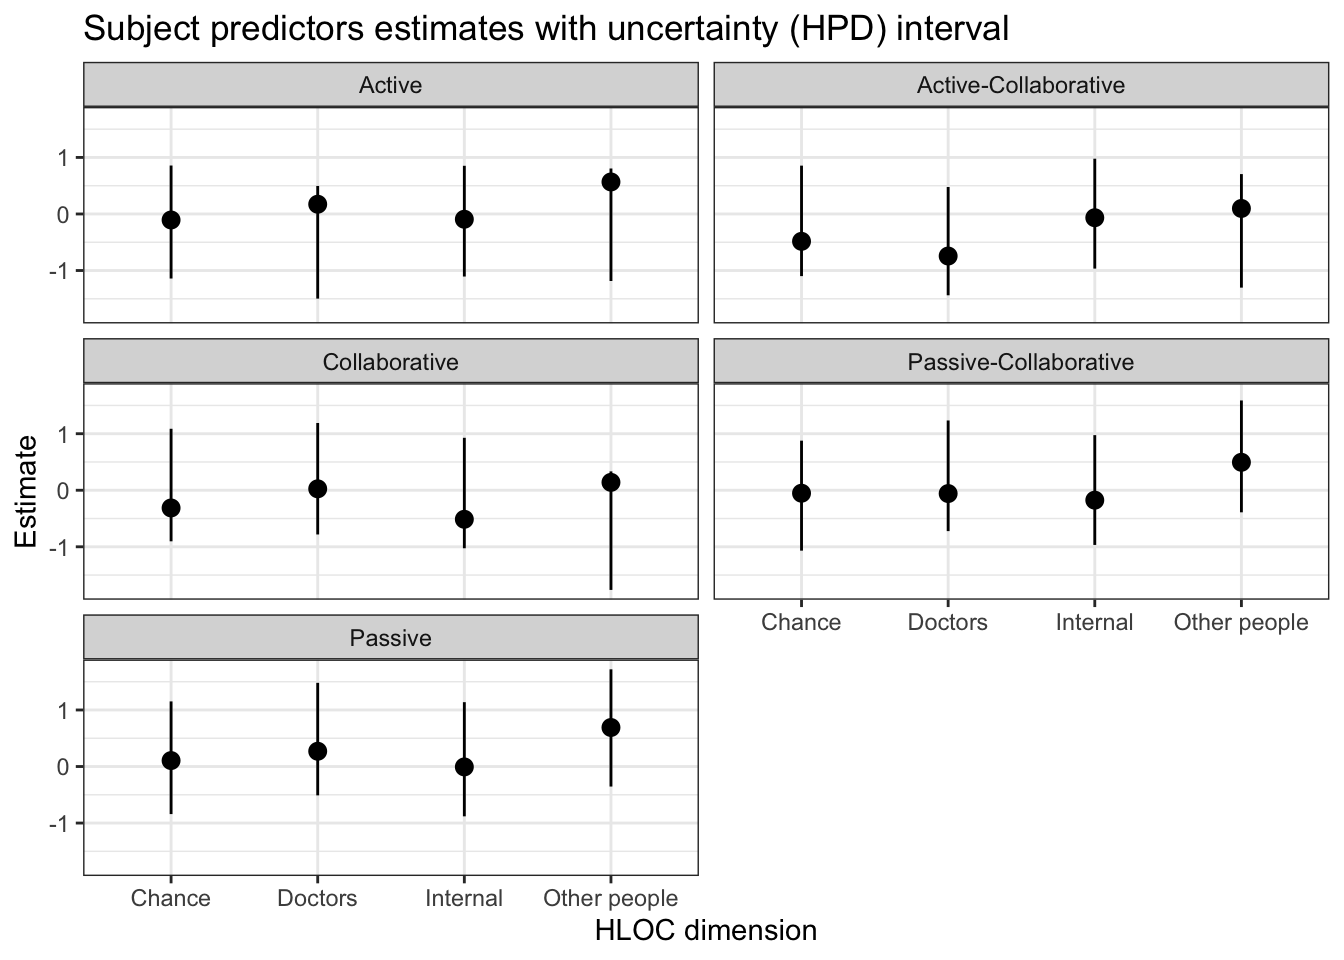
\includegraphics{bpcs-appendix_files/figure-latex/unnamed-chunk-103-1.pdf}

\hypertarget{probability-tables}{%
\subsection{Probability tables}\label{probability-tables}}

First let's create a data frame with the cases we want to investigate. We will utilize the model\_type option in the probabilities table so we can average out the values of the random effects in the subjects. In this table, we will only investigate a few of the conditions, but of course it is possible to do a much more expansive analysis

Let's create a new data frame with the conditions we want to investigate.
Mainly we are just investigating:
* Between the choice of Active and Passive how does going from -2 to 2 standard deviations over the mean influences the probability in the Internal and the Doctors
* Between the choice of Active-Collaborative and Collaborative how does going from -2 to 2 standard deviations over the mean influences the probability in the Internal and the Doctors
* Between the choice of Collaborative and Passive-Collaborative how does going from -2 to 2 standard deviations over the mean influences the probability in the Internal and the Doctors

\begin{Shaded}
\begin{Highlighting}[]
\NormalTok{newdata <-}\StringTok{ }\NormalTok{tibble}\OperatorTok{::}\KeywordTok{tribble}\NormalTok{(}\OperatorTok{~}\NormalTok{choice0, }\OperatorTok{~}\NormalTok{choice1, }\OperatorTok{~}\NormalTok{Internal, }\OperatorTok{~}\NormalTok{Chance, }\OperatorTok{~}\NormalTok{Doctors, }\OperatorTok{~}\NormalTok{OtherPeople,}
                           \StringTok{"Active"}\NormalTok{, }\StringTok{"Passive"}\NormalTok{, }\DecValTok{0}\NormalTok{, }\DecValTok{0}\NormalTok{, }\DecValTok{0}\NormalTok{, }\DecValTok{0}\NormalTok{,}
                           \StringTok{"Active"}\NormalTok{, }\StringTok{"Passive"}\NormalTok{, }\DecValTok{-2}\NormalTok{, }\DecValTok{0}\NormalTok{, }\DecValTok{0}\NormalTok{, }\DecValTok{0}\NormalTok{,}
                           \StringTok{"Active"}\NormalTok{, }\StringTok{"Passive"}\NormalTok{, }\DecValTok{2}\NormalTok{, }\DecValTok{0}\NormalTok{, }\DecValTok{0}\NormalTok{, }\DecValTok{0}\NormalTok{,}
                           \StringTok{"Active"}\NormalTok{, }\StringTok{"Passive"}\NormalTok{, }\DecValTok{0}\NormalTok{, }\DecValTok{0}\NormalTok{, }\DecValTok{-2}\NormalTok{, }\DecValTok{0}\NormalTok{,}
                           \StringTok{"Active"}\NormalTok{, }\StringTok{"Passive"}\NormalTok{, }\DecValTok{0}\NormalTok{, }\DecValTok{0}\NormalTok{, }\DecValTok{2}\NormalTok{, }\DecValTok{0}\NormalTok{,}
                           \StringTok{"Active-Collaborative"}\NormalTok{, }\StringTok{"Collaborative"}\NormalTok{, }\DecValTok{0}\NormalTok{, }\DecValTok{0}\NormalTok{, }\DecValTok{0}\NormalTok{, }\DecValTok{0}\NormalTok{,}
                           \StringTok{"Active-Collaborative"}\NormalTok{, }\StringTok{"Collaborative"}\NormalTok{, }\DecValTok{-2}\NormalTok{, }\DecValTok{0}\NormalTok{, }\DecValTok{0}\NormalTok{, }\DecValTok{0}\NormalTok{,}
                           \StringTok{"Active-Collaborative"}\NormalTok{, }\StringTok{"Collaborative"}\NormalTok{, }\DecValTok{2}\NormalTok{, }\DecValTok{0}\NormalTok{, }\DecValTok{0}\NormalTok{, }\DecValTok{0}\NormalTok{,}
                           \StringTok{"Active-Collaborative"}\NormalTok{, }\StringTok{"Collaborative"}\NormalTok{, }\DecValTok{0}\NormalTok{, }\DecValTok{0}\NormalTok{, }\DecValTok{-2}\NormalTok{, }\DecValTok{0}\NormalTok{,}
                           \StringTok{"Active-Collaborative"}\NormalTok{, }\StringTok{"Collaborative"}\NormalTok{, }\DecValTok{0}\NormalTok{, }\DecValTok{0}\NormalTok{, }\DecValTok{2}\NormalTok{, }\DecValTok{0}\NormalTok{,}
                           \StringTok{"Collaborative"}\NormalTok{, }\StringTok{"Passive-Collaborative"}\NormalTok{, }\DecValTok{0}\NormalTok{, }\DecValTok{0}\NormalTok{, }\DecValTok{0}\NormalTok{, }\DecValTok{0}\NormalTok{,}
                           \StringTok{"Collaborative"}\NormalTok{, }\StringTok{"Passive-Collaborative"}\NormalTok{, }\DecValTok{0}\NormalTok{, }\DecValTok{-2}\NormalTok{, }\DecValTok{0}\NormalTok{, }\DecValTok{0}\NormalTok{,}
                           \StringTok{"Collaborative"}\NormalTok{, }\StringTok{"Passive-Collaborative"}\NormalTok{, }\DecValTok{0}\NormalTok{, }\DecValTok{2}\NormalTok{, }\DecValTok{0}\NormalTok{, }\DecValTok{0}\NormalTok{,}
                           \StringTok{"Collaborative"}\NormalTok{, }\StringTok{"Passive-Collaborative"}\NormalTok{, }\DecValTok{0}\NormalTok{, }\DecValTok{0}\NormalTok{, }\DecValTok{0}\NormalTok{, }\DecValTok{-2}\NormalTok{,}
                           \StringTok{"Collaborative"}\NormalTok{, }\StringTok{"Passive-Collaborative"}\NormalTok{, }\DecValTok{0}\NormalTok{, }\DecValTok{0}\NormalTok{, }\DecValTok{0}\NormalTok{, }\DecValTok{2}
\NormalTok{                           )}

\CommentTok{#Now we can calculate the probabilities}
\NormalTok{prob_hloc <-}
\StringTok{  }\KeywordTok{get_probabilities_df}\NormalTok{(}
\NormalTok{    m3, }
    \DataTypeTok{newdata =}\NormalTok{ newdata,}
    \DataTypeTok{model_type =} \StringTok{'bt-subjectpredictors'}\NormalTok{) }\CommentTok{#here we are assuming zero for the random effects}
\end{Highlighting}
\end{Shaded}

\begin{Shaded}
\begin{Highlighting}[]
\NormalTok{prob_hloc }\OperatorTok\StringTok{ }
\StringTok{  }\KeywordTok{select}\NormalTok{(}\OperatorTok{-}\NormalTok{j_beats_i) }\OperatorTok\StringTok{ }
\StringTok{  }\KeywordTok{rename}\NormalTok{(}\DataTypeTok{Probability=}\NormalTok{i_beats_j) }\OperatorTok\StringTok{ }
\StringTok{  }\KeywordTok{kable}\NormalTok{(}\DataTypeTok{caption =} \StringTok{"Probabilities of selecting role i instead of j based on changes of the values of the HLOC dimensions"}\NormalTok{,}
      \DataTypeTok{digits =} \DecValTok{2}\NormalTok{,}
      \DataTypeTok{booktabs =}\NormalTok{ T) }\OperatorTok\StringTok{ }
\StringTok{  }\NormalTok{kableExtra}\OperatorTok{::}\KeywordTok{kable_styling}\NormalTok{(}\DataTypeTok{bootstrap_options =} \KeywordTok{c}\NormalTok{(}\StringTok{"striped"}\NormalTok{, }\StringTok{"hover"}\NormalTok{, }\StringTok{"condensed"}\NormalTok{, }\StringTok{"responsive"}\NormalTok{)) }\OperatorTok\StringTok{ }
\StringTok{  }\NormalTok{kableExtra}\OperatorTok{::}\KeywordTok{add_header_above}\NormalTok{(}\KeywordTok{c}\NormalTok{(}\StringTok{"Roles"}\NormalTok{ =}\StringTok{ }\DecValTok{2}\NormalTok{, }\StringTok{"HLOC dimensions"}\NormalTok{ =}\StringTok{ }\DecValTok{4}\NormalTok{, }\StringTok{" "}\NormalTok{=}\DecValTok{1}\NormalTok{)) }\OperatorTok\StringTok{ }
\StringTok{  }\NormalTok{kableExtra}\OperatorTok{::}\KeywordTok{scroll_box}\NormalTok{(}\DataTypeTok{width =} \StringTok{"100%"}\NormalTok{)}
\end{Highlighting}
\end{Shaded}

\begin{table}

\caption{\label{tab:unnamed-chunk-105}Probabilities of selecting role i instead of j based on changes of the values of the HLOC dimensions}
\centering
\begin{tabular}[t]{llrrrrr}
\toprule
\multicolumn{2}{c}{Roles} & \multicolumn{4}{c}{HLOC dimensions} & \multicolumn{1}{c}{ } \\
\cmidrule(l{3pt}r{3pt}){1-2} \cmidrule(l{3pt}r{3pt}){3-6}
i & j & Internal & Chance & Doctors & OtherPeople & Probability\\
\midrule
Active & Passive & 0 & 0 & 0 & 0 & 0.85\\
Active & Passive & -2 & 0 & 0 & 0 & 0.80\\
Active & Passive & 2 & 0 & 0 & 0 & 0.71\\
Active & Passive & 0 & 0 & -2 & 0 & 0.96\\
Active & Passive & 0 & 0 & 2 & 0 & 0.31\\
\addlinespace
Active-Collaborative & Collaborative & 0 & 0 & 0 & 0 & 0.14\\
Active-Collaborative & Collaborative & -2 & 0 & 0 & 0 & 0.21\\
Active-Collaborative & Collaborative & 2 & 0 & 0 & 0 & 0.25\\
Active-Collaborative & Collaborative & 0 & 0 & -2 & 0 & 0.39\\
Active-Collaborative & Collaborative & 0 & 0 & 2 & 0 & 0.10\\
\addlinespace
Collaborative & Passive-Collaborative & 0 & 0 & 0 & 0 & 0.86\\
Collaborative & Passive-Collaborative & 0 & -2 & 0 & 0 & 0.84\\
Collaborative & Passive-Collaborative & 0 & 2 & 0 & 0 & 0.94\\
Collaborative & Passive-Collaborative & 0 & 0 & 0 & -2 & 0.99\\
Collaborative & Passive-Collaborative & 0 & 0 & 0 & 2 & 0.43\\
\bottomrule
\end{tabular}
\end{table}

  \bibliography{book.bib,packages.bib}

\end{document}
